\documentclass[10pt,a4paper,twocolumn]{article}
\usepackage[utf8]{inputenc}
\usepackage[english]{babel}
\usepackage{amsmath}
\usepackage{amsfonts}
\usepackage{amssymb}
\usepackage{makeidx}
\usepackage{natbib}
\usepackage{graphicx}
\usepackage{hyperref}
\usepackage{lscape}
\usepackage{appendix}
\usepackage{midpage}
\usepackage{gensymb}
\usepackage{geometry}
\usepackage{color}
\usepackage{tabularx}
\usepackage{footmisc}
\geometry{top=1cm, bottom=2cm, left=1.5cm, right=1.5cm}
\setlength{\columnsep}{1cm}
\setlength{\extrarowheight}{3pt}
\setcitestyle{square}


\author{Matteo Malucchi \hspace{2.5cm}  Lorenzo Punzi}
\title{\textbf{MU DECAY}}
\begin{document}
\date{May 2022}

\twocolumn[
  \begin{@twocolumnfalse}
  \maketitle
    \begin{abstract}
      \noindent The lifetime of cosmic ray muons and antimuons has been measured in different materials through the observation of the decays $\mu^- \rightarrow e^- + \overline{\nu}_e+ \nu_{\mu}$ and $\mu^+ \rightarrow e^- + \nu_e+ \overline{\nu}_{\mu} $. The measurements of $\tau_{\mu^+}$ were found to be compatible between different materials, and yield the final point estimate $\tau_{\mu^+}=2.20  \pm 0.03 \text{ (stat)} \pm 0.11 \text{ (syst) }\mu$s. Also, measurements of $\tau_-$ where executed in different materials, finding some values not compatible with each other and others compatible with tabulated measurements. Also, the effects of P violation in weak interactions were observed, along with the charge ratio of incoming muons.
      \bigskip
      \bigskip
      \bigskip
     
    \end{abstract}
  \end{@twocolumnfalse}
]

\section{Apparatus}

For this experiment the apparatus used was divided in two parts, each in a different room. The detector (Figure \ref{detector}) is a set of rectangular plastic scintillators (about 40cm x 48cm x 1.5cm), each connected to its own PMT by a light guide. These scintillators are stacked horizontally on a rack, equidistant from one other at a distance of about 10 cm (with two exceptions being PMT 1 and PMT 7). In the space between the scintillators there is room to fit similarly shaped slabs of materials used for the purposes of this experiment. The bottom scintillator (attached to PMT 1), is farther down, at almost 40 cm from PMT 2. A much smaller scintillator (about 4cm x 4cm) attached to PMT 7, that can easily be moved around, is also present. 

\begin{figure}[h!]
\centering
\includegraphics[scale=0.14]{Lab4/Mudecay/Detectorrack.jpeg} 
\caption{Detector rack scheme with distances in [cm]}
\label{detector}
\end{figure}



The slabs of materials used were Fe, Al, a mixture of Al+Pb (1 mm:3 mm in thickness), NaCl (in store bought salt boxes) and "magnetized" Fe. The latter is a magnetic circuit composed of two slabs of Fe attached together and a set of Nd magnets attached to them (see Figure \ref{magnetizedFe}).

\begin{figure}[h!]
\centering
\includegraphics[scale=0.16]{Lab4/Mudecay/Magslab.png} 
\caption{Sketch of the magnetized Fe slabs}
\label{magnetizedFe}
\end{figure}

\noindent The electronic circuit to identify and register the passing and decaying of cosmic muons was built in a different room. For this purpose NIM logic was used, as well as an oscilloscope (an example of an observed waveform is shown in Figure \ref{WAVE}), a De0-Nano board and a NIM to TTL converter for the board. The data was registered on a computer using the analogic ports of the De0-Nano. The full list of modules used can be found in Appendix \ref{appendix:nimmodules}.

\begin{figure}[h!]
\centering
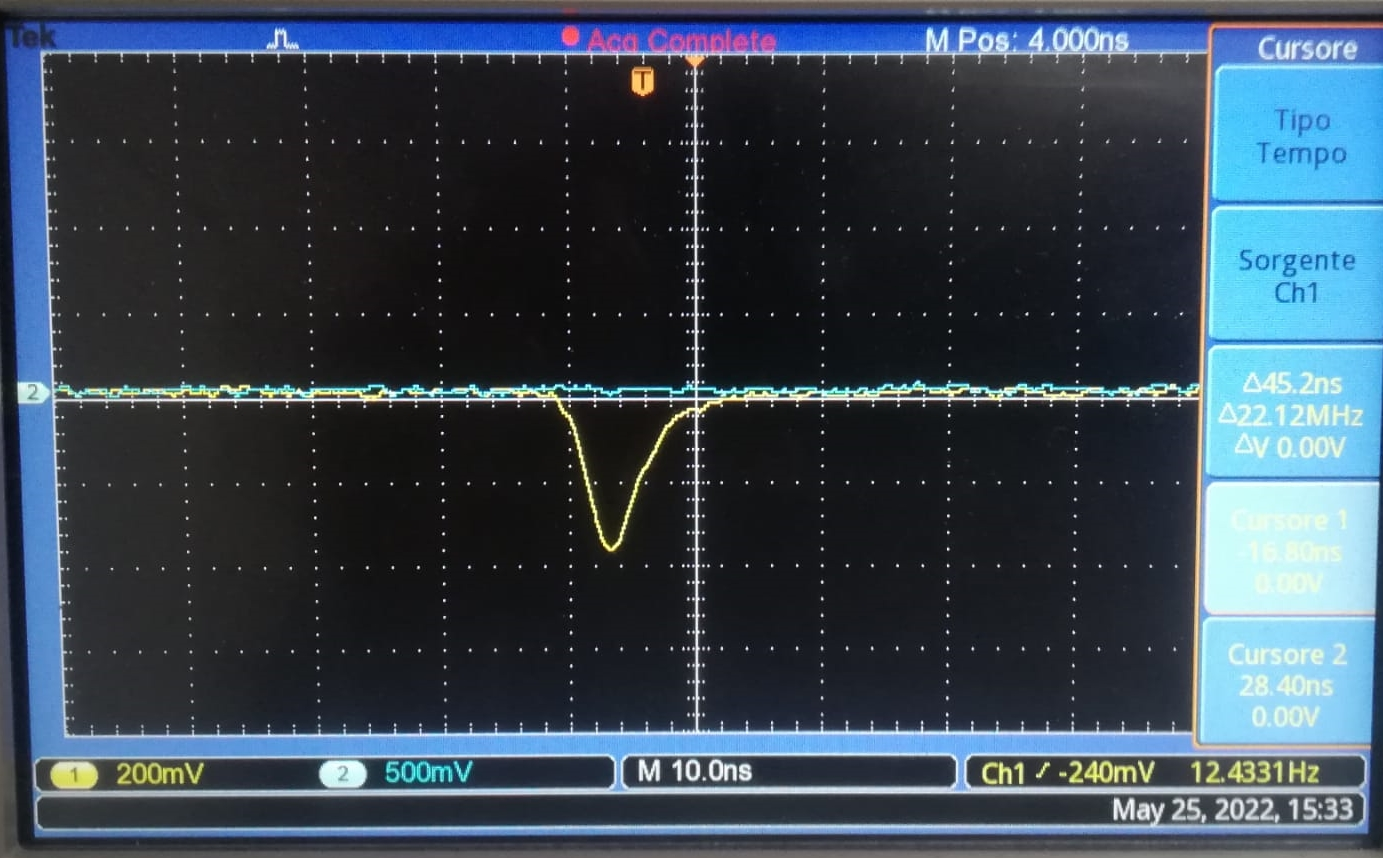
\includegraphics[scale=0.2]{Lab4/Mudecay/wave.jpeg} 
\caption{Example of waveform observed at the oscilloscope. [25/05/22]}
\label{WAVE}
\end{figure}

\section{Introduction}

Sea level cosmic rays are, excluding neutrinos, made up of muons for $\simeq$99\%. The relative abundances of the two components are expected to be around $N_+/N_- \simeq 1.27$ \cite{CMSarticle}. The energy spectrum of such muons is reported in \figurename~\ref{muspectrum}. The average energy of these muons is $\sim$ 4 GeV, so losing only $\sim$ 2 MeV  cm$^2$/g at MIP most of them pass right through any slab of material available. It is however possible to stop the ones with low energy (with a few cm of material the maximum energy stoppable is $\sim$ 40 MeV), which then all decay in the span of a few lifetimes without relativistic time dilation. Muons (essentially) always decay as

\begin{equation}
    \mu^- \rightarrow e^- + \overline{\nu}_e+ \nu_{\mu} \quad , \quad \mu^+ \rightarrow e^- + \nu_e+ \overline{\nu}_{\mu} 
\end{equation}

\begin{figure}[h!]
\centering
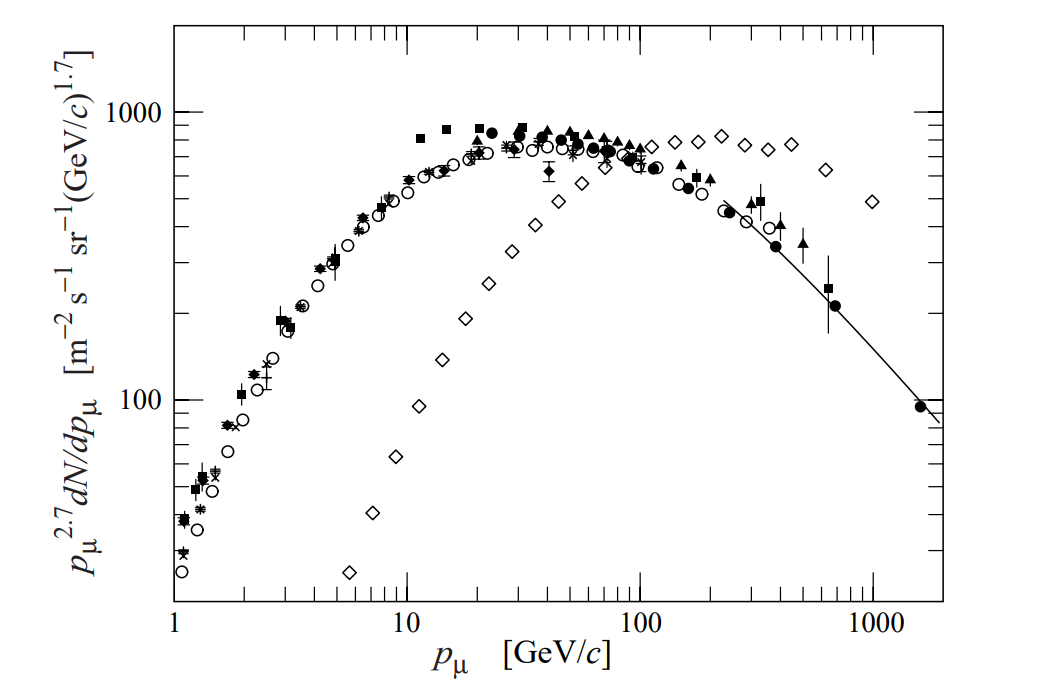
\includegraphics[scale=0.4]{Lab4/Mudecay/muon_spectrum.png} 
\caption{Spectrum of muons at $\theta$ = 75\degree ($\diamondsuit$) and $\theta$ = 0° (all the other symbols). Notice that the quantity on the $y$ axis is multiplied by $p_\mu$ itself. \cite{PDG_spectrum}}
\label{muspectrum}
\end{figure}

Using a well timed circuit it is possible to observe muons stopping in a slab of material placed between two scintillators and the subsequent $e^{\pm}$ activating the scintillators either directly above or below said slab. Thus, the distribution of the difference in time between the detection of the $e^\pm$ and the incoming $\mu^\pm$ can be recorded.
\\
\\
The lifetime of muons in vacuum is 2.197 $\mu$s \cite{PDGtau}. However in matter, due to the electromagnetic interaction between $\mu^-$ and the matter's nuclei, the lifetime of $\mu^-$ is shorter\footnote{The authors were not able to find an in depth measurement of the lifetime in NaCl, the results of other similar experiments have been used as reference point for NaCl.}, as shown in Table \ref{mulifetimematerials}.



\begin{table}[h]
\centering
\begin{tabular}{|c|c|}
\hline
MATERIAL & LIFETIME [$\mu s$]   \\
\hline
Vacuum & $2.196981 \pm 0.000002$ \\
Fe &  $0.201 \pm 0.004$   \\
Al &  $0.88 \pm 0.01$  \\
Pb &  $0.0749 \pm 0.0004$   \\
NaCl &  $\sim 0.7$   \\
\hline
\end{tabular} 
\caption{Muon lifetime in different materials }
\label{mulifetimematerials}
\end{table}

\\
The $\mu^+$ are immune to this effect, so their lifetime is the same in matter as it is in vacuum. Therefore for a given material two decay times are expected to be observed in the time distribution recorded: the vacuum lifetime ($\mu^+$ component, $\tau_+$) and the reduced one ($\mu^-$ component, $\tau_-$).
\\



\section{Initial setup and working point}

In order to have good efficiencies without having too noisy data a suitable working point must be chosen for each PMT. In principle this can be done by studying a F.O.M. while varying the threshold of the discriminator where PMT pulses are sent and/or the power supply voltage of the PMT itself. In this case the thresholds were held constant at -30 mV and instead the voltages were varied. 

The procedure for choosing a working point for each scintillator is as follows: the number of double coincidences between the two neighboring scintillators in a given time interval is measured, along with the triple coincidences between said scintillators and the scintillator in the middle. The former will be called $N$ and the latter $n$.
\\
The ratio $\xi=n/N$ is expected to always be no bigger than 1 and depends on the power supply of both the scintillator and its neighbors. The dependence on the power supply of the neighbors is due to the fact that not all of the $N$ counts are actually signal, some is inevitably background noise due to casual overlapping of individual noise in the two detectors. This dependence can be observed in Figure \ref{volteffdepend}, where the red point is obtained by simply changing the power supplies of the neighboring PMTs. Since the efficiency $\varepsilon$ of the detector can depend on its voltage but \textit{not} the one of its neighbors, it is clear that $\xi$ is not a good estimator for $\varepsilon$, or at least not in this regime. One could measure the individual frequencies and subtract the expected casual coincidences from $N$ in the evaluation of $\xi$, and this would solve the problem. Of course this ignores the possibility of \textit{triple} casual coincidences, which are a correction of the next order.

\begin{figure}[h!]
\centering
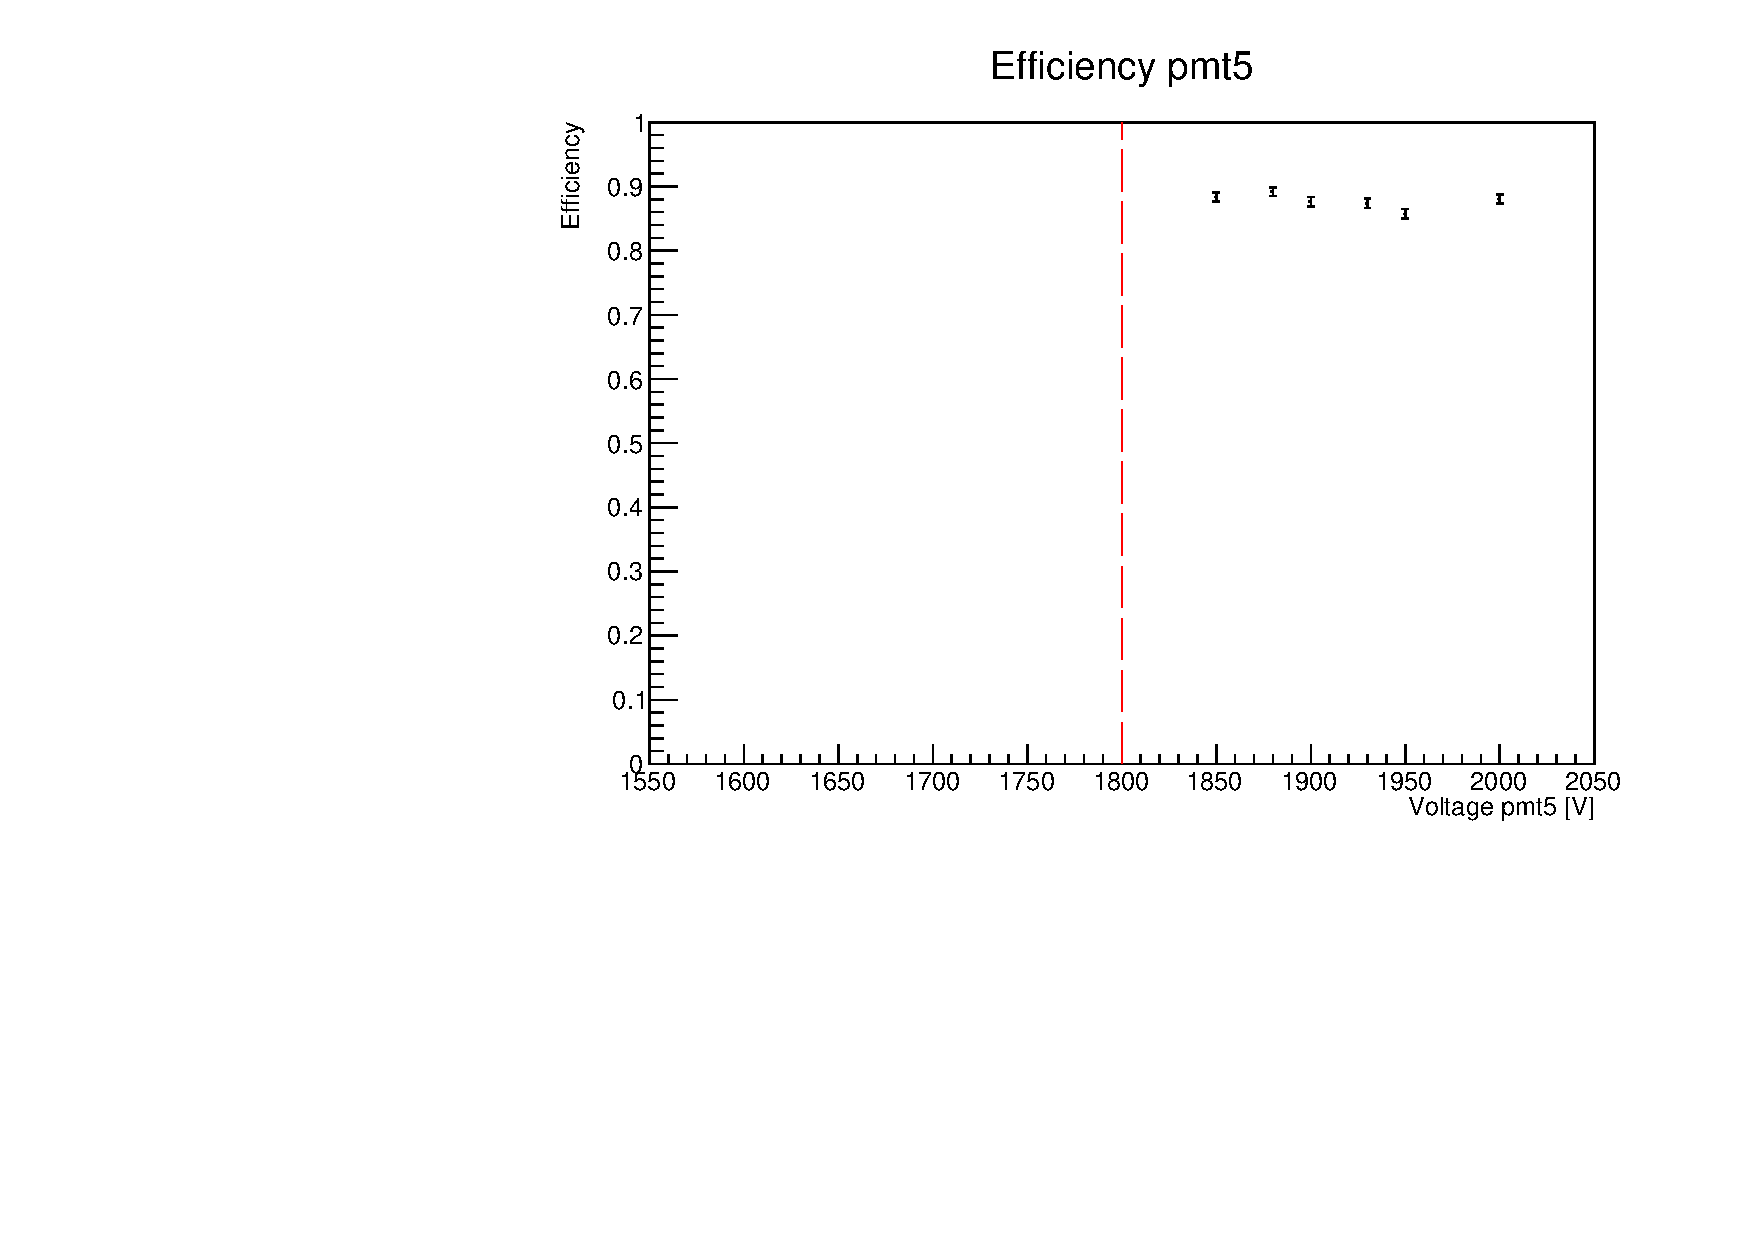
\includegraphics[scale=0.4]{Lab4/Mudecay/pmt5_efficiency.pdf} 
\caption{Efficiency plot for PMT 5 as a function of its voltage. The black points represent the estimate of the efficiency when the voltages of the neighbors are $V_4 = 1750 $ V  and  $V_6 = 1800 $ V, while the red one is obtained by varying the voltages to  $V_4 = 1650 $ V  and  $V_6 = 1700 $ V. The blue dotted line represents the working point that was chosen. [03/05/22]}
\label{volteffdepend}
\end{figure}

\\
However, the objective here is \textit{not} that of measuring $\varepsilon$. It is instead to find the optimal working point for the scintillator. To do this $\xi$ is measured at different supply voltages of the central scintillator while keeping the voltages of the neighbors constant. The profiles are all similar to the one in Figure \ref{volteffdepend}. The optimal working point is chosen to be at the voltage at which $\xi$ stops increasing and reaches the knee just before an approximately constant plateau. This is because the initial slope is due to an increase in signal: if it were due to noise it wouldn't stop increasing at a certain point and become constant. Having reached the plateau it is therefore useless to raise the voltage further, as that could only contaminate the signal further with excess noise. This "knee voltage" is independent of the voltage of the neighboring detectors, which does nothing but shift the profile up or down. The voltages set for the PMTs are as shown in Table \ref{voltworkpoints}. In the Table are also reported the $\xi$ measured for said working points, even if as mentioned before these are not actually estimates of $\varepsilon$. For PMTs 1 and 7 $\xi$ is much lower than the others because they are not sandwiched between two scintillators, but the two nearest scintillators are used instead. The sudden decrease in $\xi$ is therefore due to the \textit{geometrical} component of the efficiency being lower in such configuration.

\begin{table}[h]
\centering
\begin{tabular}{c|c|c}
PMT & $V_{supply}$ [V] & $\xi$  \\
\hline
1 &  1850  &  0.2   \\
2 &  1700  &  0.9   \\
3 &  1750  &  0.6   \\
4 &  1750  &  0.8   \\
5 &  1650  &  0.8   \\
6 &  1750  &  0.9   \\
7 &  1700  &  0.03   \\
\end{tabular} 
\caption{Supply voltages chosen as working points}
\label{voltworkpoints}
\end{table}


Another important aspect of the initial setup is making sure that the scintillators are all \textit{in time} relative to each other. This means making sure that when a cosmic muon passes through all scintillators the signals emitted by the PMTs arrive at the NIM circuit not too far apart in time. How much "too far apart" means depends on a few factors. They cannot be farther apart than the duration set for their NIM signals. Since the discriminated pulse signals are set to last about 25 ns it is necessary for the maximum relative distance between any two PMTs to be less than so. However since the muon itself takes around 3-4 ns to pass through the whole rack, it is overkill to sync them better than that. The signals were found to be already within 5 ns from a same reference PMT (PMT 2). Only rarely some were found at 10 ns, which is still good enough for the purposes of this measurement. 
\\
\\
At this point the correct functioning of the detectors and their timing was tested. To do this the rate of 6&5&4&3&2 events was measured and compared to the approximate expected value given the surface of the detectors and their $\xi$, even if the $\varepsilon$ were still unknown at the time. The results found are $N_{measured} = 840$ and $N_{expected}\sim 1015$. While these results aren't terrible (within 20 \%), it stops making sense when the actual values that should be expected, based on the efficiencies in (\ref{eff_meas}) (around $N_{expected}=2564$), differ much more (a factor of 3) from what is measured.





\section{Measurement of $\tau_\pm$}

At this point the main objective was to build a NIM circuit capable of accurately registering a few key times through the De0-Nano board. The first is the time at which a muon passes through detectors above slabs of a given material but doesn't pass through the ones underneath it: this is called the START signal. The second time is the one at which, following the START signal, detectors above or below are triggered by the $e^\pm$ that comes from the decay of said $\mu^\pm$: these are called respectively STOPUP and STOPDOWN signals. The time difference between STOP signals and their START is called $t$, and its distribution is fitted to measure $\tau_+$ and $\tau_-$. An example of such distribution is shown in Figure \ref{exampletdistr}.

\begin{figure}[h!]
\centering
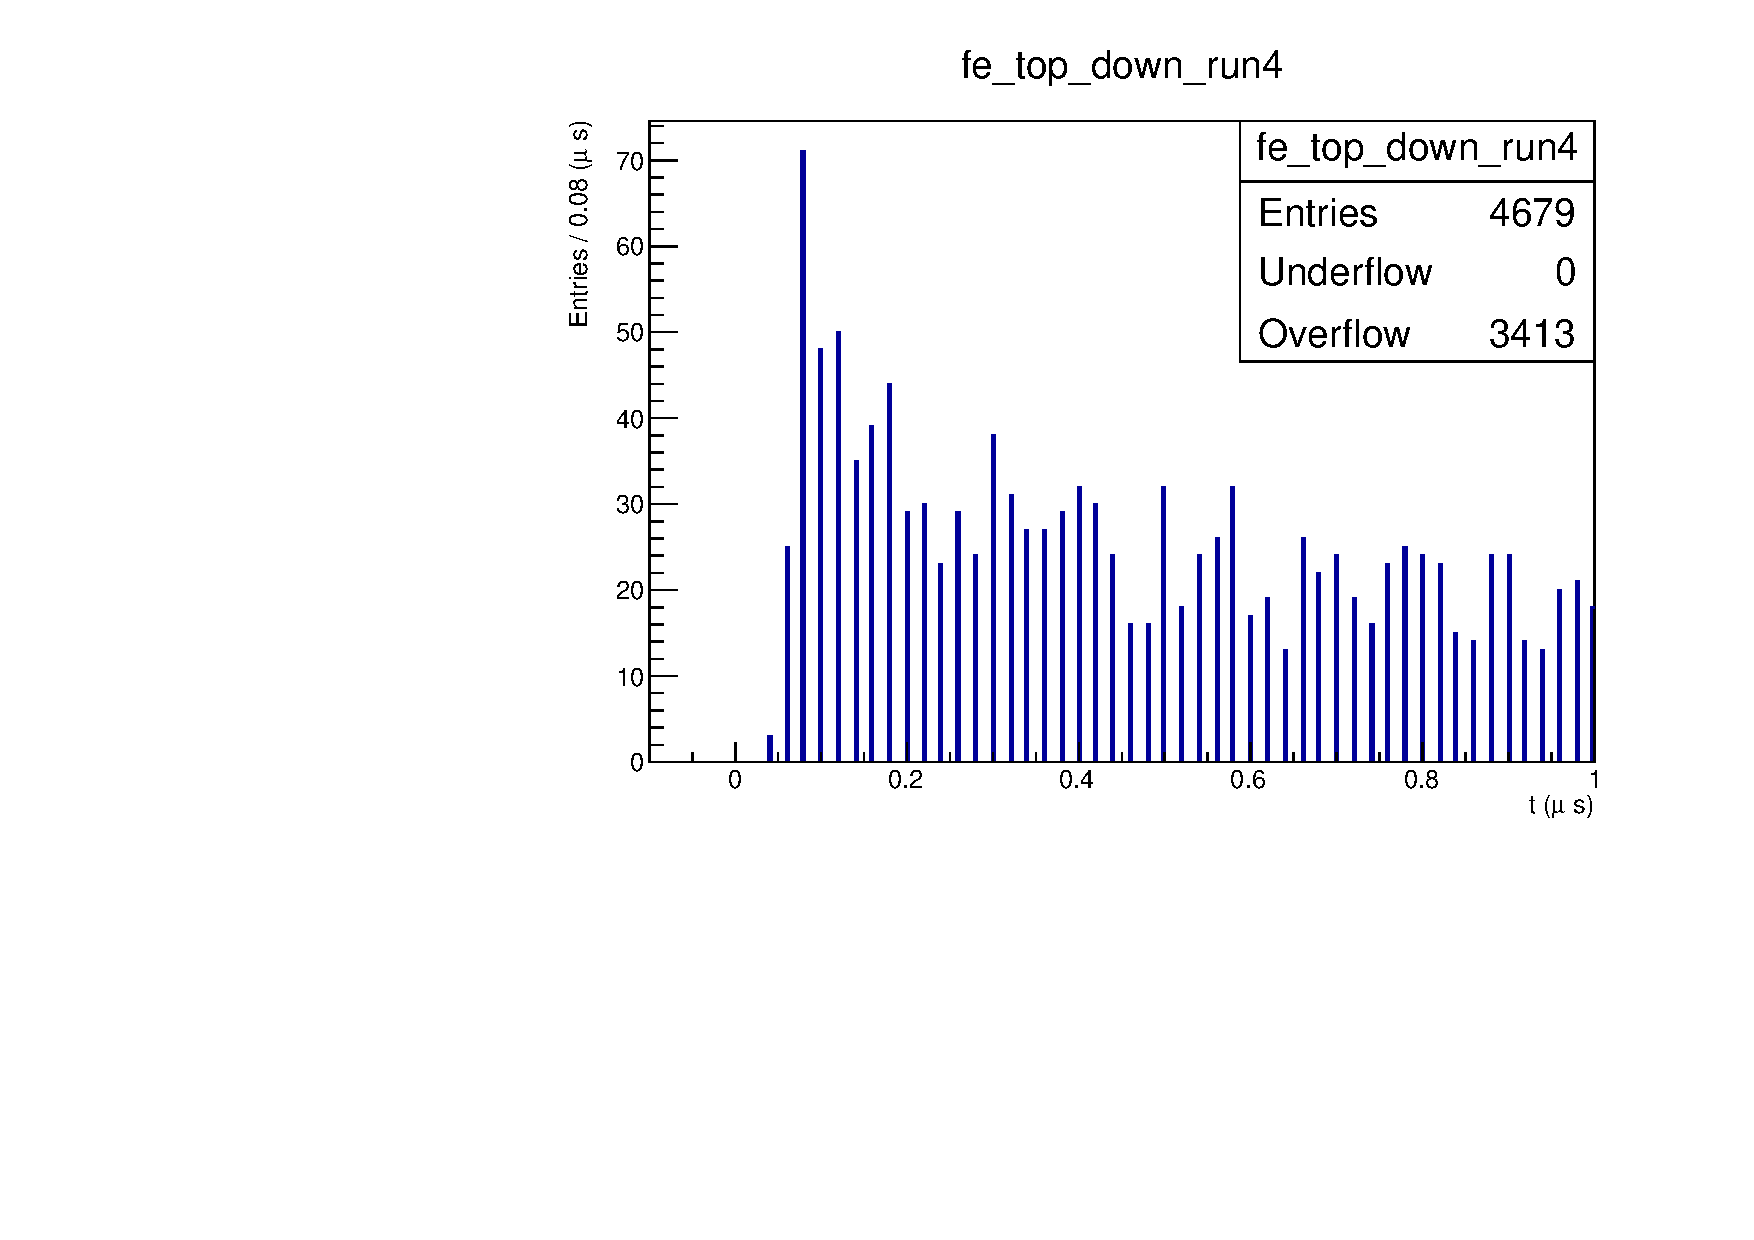
\includegraphics[scale=0.4]{Lab4/Mudecay/fe_top_down_run4.pdf} 
\caption{Example of a time distribution obtained as explained in the text. For this measurement were used 4 Fe slabs put in the TOP section. [17/05/22]}
\label{exampletdistr}
\end{figure}

The board is programmed to print on a \texttt{.dat} file a column of events, made up of a channel number and a timestamp at which the board reads on said channel's analog port a TTL signal on it. The time stamp resolution is 20 ns, which is not a problem since the shortest lifetime measure is expected to be the iron's $\tau=201 \pm 4$ ns. The amount of Fischer information of an exponential lost with bins large 1/10 of the lifetime is less than 0.1\%, so it doesn't noticeably increase the uncertainty on the fitted parameters.
\\
\\
Due to various phenomena the $t$ measured do not exactly correspond to the lifetimes of the various $\mu^\pm$ decaying in the apparatus, and hence its distribution (Figure \ref{exampletdistr}) is not expected the be the sum of two exponentials ($\tau_+$ and $\tau_-$).
\\
First of all, there are events in which the STOP signal is uncorrelated with the START one. This is due to the firing of the STOP scintillators during the time frame observed (see GATE later) not because of a $e^\pm$ but either due to the passing of a cosmic muon or a coincidental random noise signal in the scintillators. This is the main source of background, and it has a uniform distribution, which dominates the spectrum at $t$ bigger than a few long lifetimes $\tau_+\sim 2$ $\mu$s. This can be taken in consideration by simply adding a constant to the fitting model used. The fact that the constant component of the measured $t$ distribution is precisely due to this type of background can be checked. This is done by comparing the number of expected background events to the actual offset measured in the distribution. The details of this procedure are outlined in Appendix \ref{appendix:combinatorial}. 
\\
Since the muon takes time to stop from when it is first detected (START), this time is added to $t$ but has nothing to do with the lifetime of the $\mu^\pm$, which is measured assuming there is no time dilation (the muon is at rest). It can however be shown (Appendix \ref{appendix:stoptime}) that this stopping time is of the order of less than 1 ns, so it is completely negligible compared to the times in question and even the board's resolution itself.
\\
Also, the $e^\pm$ emitted from the decay take a finite amount of time to reach the scintillators above or below the slab, activating the STOP signal. Since the $e^\pm$ have $\beta \simeq 1$  this time is shorter than 10 cm/c, which is fractions of a ns, so it is again negligible.
\\
Furthermore, the time it takes for the pulses to travel from the PMTs to the circuit can't be exactly the same, and this biases $t$. However, as discussed in the previous section, this time is no more different than 5 ns, which is still small compared to the lifetimes measured and to the resolution of the board itself.
\\
Finally, in the circuit, which will be described in detail in the next section, it is important that the different paths of the START and STOP signals have the same (temporal) length. This mainly has an effect on the coefficients of the exponentials rather than on the lifetimes itself, since a shifted exponential is \textit{still and exponential} but with different coefficient (equation \ref{exposhift}). The maximum difference in cable timing is found to be 5 ns, which is negligible compared to the lifetimes in question and is even 4 times smaller than the resolution of the board.


\section{NIM circuit}

The NIM circuit was designed to be able to record data for two different slabs of materials simultaneously, as show in Figure \ref{detectwslabs}.

\begin{figure}[h!]
\centering
\includegraphics[scale=0.18]{Lab4/Mudecay/detectrack.jpeg} 
\caption{Schematization of the detector rack with two slabs of material simultaneously}
\label{detectwslabs}
\end{figure}


It also measures the efficiencies of PMTs $5\cdot 6$, $3\cdot 4$ and 2 in real time. The two different sections, dedicated to measuring lifetimes in the top and the bottom slab, will be called respectively TOP and BOT. 
\\
A general scheme of the circuit is shown in Figure \ref{circuitscheme}

\begin{figure*}[h!]
\centering
\includegraphics[scale=0.28]{Lab4/Mudecay/Circuitscheme.png} 
\caption{Schematization of the NIM circuit employed}
\label{circuitscheme}
\end{figure*}


\subsection{Time difference acquisition}

Part of the function of the circuit is then that of correctly generating START, STOPUP and STOPDOWN signals for both TOP and BOT. These correspond to what is shown in Table \ref{signaltable}


\begin{table}[h]
\centering
\begin{tabular}{|c|c|c|c|}
\hline
\multicolumn{2}{|c|}{TOP}&\multicolumn{2}{|c|}{BOT}\\
\hline
START &  $6\cdot 5\cdot \overline{4}\cdot \overline{3}$ & START & $4\cdot 3\cdot \overline{2}\cdot \overline{1}$\\
\hline
STOPUP & $6\cdot 5$ & STOPUP  &  $4\cdot 3$   \\
\hline
STOPDOWN & $4\cdot 3$ & STOPDOWN  &  2   \\
\hline
\end{tabular} 
\caption{Meaning of the signals used}
\label{signaltable}
\end{table}

In building the START signals it is necessary for the VETO signals, the ones that are negated, to be larger in duration than the non VETO ones, and that the latter be completely contained in the former. If it were not so there would be a risk of an accidental START signal when in reality there was a signal in the VETO scintillators after all. This is illustrated in Figures \ref{vetobad} and \ref{vetogood}.

\begin{figure}[h!]
\centering
\caption{Case of presence of signal (in blue) on VETO (in red) that is mistaken for the absence of signal}
\includegraphics[scale=0.13]{Lab4/Mudecay/vetobad.jpeg} 
\label{vetobad}
\end{figure}

\begin{figure}[h!]
\centering
\caption{Case of absence of signal (in blue) on VETO (in red) that is correctly interpreted}
\includegraphics[scale=0.22]{Lab4/Mudecay/Vetogood.jpeg} 
\label{vetogood}
\end{figure}





To achieve this the VETO signals are extended to a duration of 350-400 ns \footnote{It is a duration much shorter than the typical time distance between consecutive events, which is more than a ms . This ensures that a START signal doesn't cause a later event in which the muon actually passed through the VETO to appear as a START signal as well. \label{foottimedist}} and the single PMT channels that aren't vetoed are \textit{delayed} by 30 ns, so that the START signal is delayed by the same amount. This requires that the STOP signals too be delayed by the same amount, otherwise $t$ would be biased by 30 ns. This is exactly what was done, but only \textit{nominally}, that is without taking into account the different temporal lengths of the cables used for the different signals. Accounting for the cables the differences, as mentioned in Section 4, are negligible for the purposes of the experiment.


The use of more than just one VETO scintillator is because this reduces the possibility of misinterpreting the event due to inefficiencies, cutting therefore part of the noise, while also not reducing the signal at all.
\\
\\
The use of more than one scintillator for STOP when possible (it is not practical for STOPDOWNBOT due to PMT 1 being so far away) serves to suppress the influence of \textit{afterpulses}. Afterpulses in PMTs are pulses that follow actual signal pulses. Electrons flowing in the PMT ionize its gas atoms. These ions drift to the photocathode under the effect of the PMT's voltage and release secondary electrons on impact. This happens after a certain delay, which depends on the specific ion produced but does not strongly depend on the location where the ion was produced, due to the profile of the electric field. The delay is usually of the order of hundreds of ns.
\\
\\
An important limiting factor of the De0-Nano board is that it has a limited bandwidth, with a maximum frequency in the tens of Hz. If one exceeds said limit it is possible that the board's buffer into the computer gets jammed by data and the data file given by the program could be nonsensical from a certain point forward. In these cases the data was cut at the point at which it begins to be meaningless. For this reason it is not convenient to blindly record every STOP signal present: a GATE signal is used to limit acquisition rate. This signal is nothing but the START signal delayed and extended to a duration of 30 $\mu$s. Were it not for the presence of the GATE, the frequency of STOP signals would be that of the PMTs that are used for STOP. From measurements made with multiscalers these are known to be, for $5\cdot 6$ and $3\cdot 4$, about 20 Hz. This would lead to total bandwidth greater than what the board can handle without great risk of failure.
\\
\\
The delay is necessary because the STOPUP signal is always activated when a START signal is activated by definition. Thus there would always be a STOPUP signal at the beginning of GATE's window of time that corresponds to the passing of the muon itself, not of a later $e^\pm$. The size of this delay was 50 ns to start but was later decreased to 40 ns when the START signals were made 20 ns long.
\\
The duration was set to 30 $\mu$s because it fits certain appealing criteria. It is much smaller than the typical time between consecutive cosmic rays passing through our detectors, as detailed in Footnote \footref{foottimedist}, so that it doesn't record as STOP signals later cosmic muons passing through. It is also $\sim$ 15 lifetimes long, so that the Fischer information lost on the exponential is less than 0.01\%.

\subsection{Efficiency measurement}

In order to evaluate the efficiencies of the detectors part of the NIM circuit is dedicated to registering on a multiscaler coincidence counts. Since PMTs 5\&6 and 3\&4 are always used together as a couple, the efficiency of the couples as a whole was evaluated. The efficiencies are estimated as follows


\begin{equation}
    \label{effcalc}
    \varepsilon_{65}=\frac{N_{76543}}{N_{743}} \quad , \quad\varepsilon_{43}=\frac{N_{65432}}{N_{652}} \quad , \quad \varepsilon_2=\frac{N_{4321}}{N_{431}}
\end{equation}

\noindent In this evaluation the number of casual coincidences is neglected since they are at least coincidences of 3 scintillators. This suppresses casual coincidences by a factor of $f_3 \delta \tau$, which for the numbers in question is around $10^{-4}$ counts. Efficiency measurements were executed as described for each run, regardless of the materials used. These were found to be consistent between runs.
The statistical uncertainties of the efficiencies were evaluated using a binomial approximation

\begin{equation}
    \hat{\varepsilon}=\frac{n}{N} \longrightarrow Var(\hat{\varepsilon})=\frac{Var(n)}{N^2}=\frac{\varepsilon(1-\varepsilon)}{N}
\end{equation}

and then all results were united from different runs weighting them with the inverse of their variance.

Due to limited space, the counts at the denominators in (\ref{effcalc}) had to be taken not by sending OUT signals from NIM AND modules to the multiscaler but by sending it $\overline{\text{OUT}}$. Ideally, this shouldn't make a difference, minus possibly one or two counts. Instead when sending the same signal as OUT and $\overline{\text{OUT}}$ simultaneously a difference of between 1/4000 and 6/4000 counts was found. This difference varies wildly from run to run for reasons unknown to the authors of this work. This means that the numbers acquired for $N$ are \textit{not actually} $N$. This can be taken in consideration by simply adding to the efficiencies a systematic uncertainty of the order, to be conservative, of 6/4000. This error has little influence over the use of the efficiencies made in this work , since the objective is not to measure with great precision rates of events, but it is the dominant source of error on the efficiencies.


\begin{equation} \label{eff_meas}
\begin{split}
\varepsilon_{56} &=0.882 \pm 0.001 \\
\varepsilon_{34} &=0.942 \pm 0.001 \\
\varepsilon_2 & =0.931\pm 0.001
\end{split}
\end{equation}




\section{Measurement of $\tau_+$}

Since in any of the materials used $\tau_-$ is lower than $\tau_+$, at high enough $t$ the distribution is equal to just the longer exponential plus a constant to very good approximation.

\begin{equation}
    \label{expo_long}
    p(t)=\Lambda_+ e^{-t/\tau_+}+\Lambda_0
\end{equation}


Fitting only at higher $t$ allows for an easier fit since the sum of two exponentials is well known to be a particularly difficult model to fit correctly. The only problem is that if $\tau_-$ is too similar to $\tau_+$, in order to suppress the former one must go so high that the latter becomes difficult to fit as well. For this reason Fe, in which $\tau_-/\tau_+\sim 1/10$, is particularly suitable for this purpose.
\\
\\
The types of fits executed for the following measurements of both $\tau_+$ and $\tau_-$ are detailed in Appendix \ref{appendix:fitmethods} and the specifics of the various runs in Appendix \ref{appendix:runs}.

\subsection{Systematic uncertainties}

A form of systematic uncertainty considered while measuring $\tau_+$ is the one that arises from the arbitrary choice of the fitting interval. Both extremities were varied, the lower one within the interval of $\pm 0.2$ $\mu s$ around the central value, indicated in the caption of the figures, by steps of 0.1 $\mu s$ and the upper one between [24, 30] $\mu s$ by steps of 1 $\mu s$. An analogous procedure was applied to all the materials that follow. On top of that, when fitting $\tau_-$ the lower extremity from which the short-lifetime fit starts, is also varied in the interval $\pm 0.03 \mu s$ around its central value by steps of 0.02 $\mu s$.
\\
\\
Another systematic uncertainty is the one on the fitting model itself. Specifically, since support beams \footnote{For each slot (TOP/BOT) 2 bars 5 x 46.5 x 0.5 cm$^3$} were present throughout the detector rack it is possible that they contaminate the data with an additional (albeit small) component with another lifetime. The support beams are of an unknown metal; if they were made of iron this contamination wouldn't change the substantial nature of the $t$ distribution for Fe. This contamination \textit{cannot} be relevant in this particular measurement because the interval are always chosen at high enough $t$ that Fe $\tau_-$ has no influence there.


\subsection{$\tau_+$ from Fe}

First, the procedure was executed on Fe, placed in TOP position, with the total collected data for STOPUP and STOPDOWN separately, putting together all runs. The results found are shown in Figures \ref{FEUP} and \ref{FEDWN} and a discussion on the thickness of the Fe slabs and all the other slabs can be found in Appendix \ref{appendix:slabthickness}

\begin{figure}[h!]
\centering
\caption{Time distribution of Fe TOP UP fitted in the range [0.9, 30] $\mu s$. [10-11-12-17-19-26/05/22]}
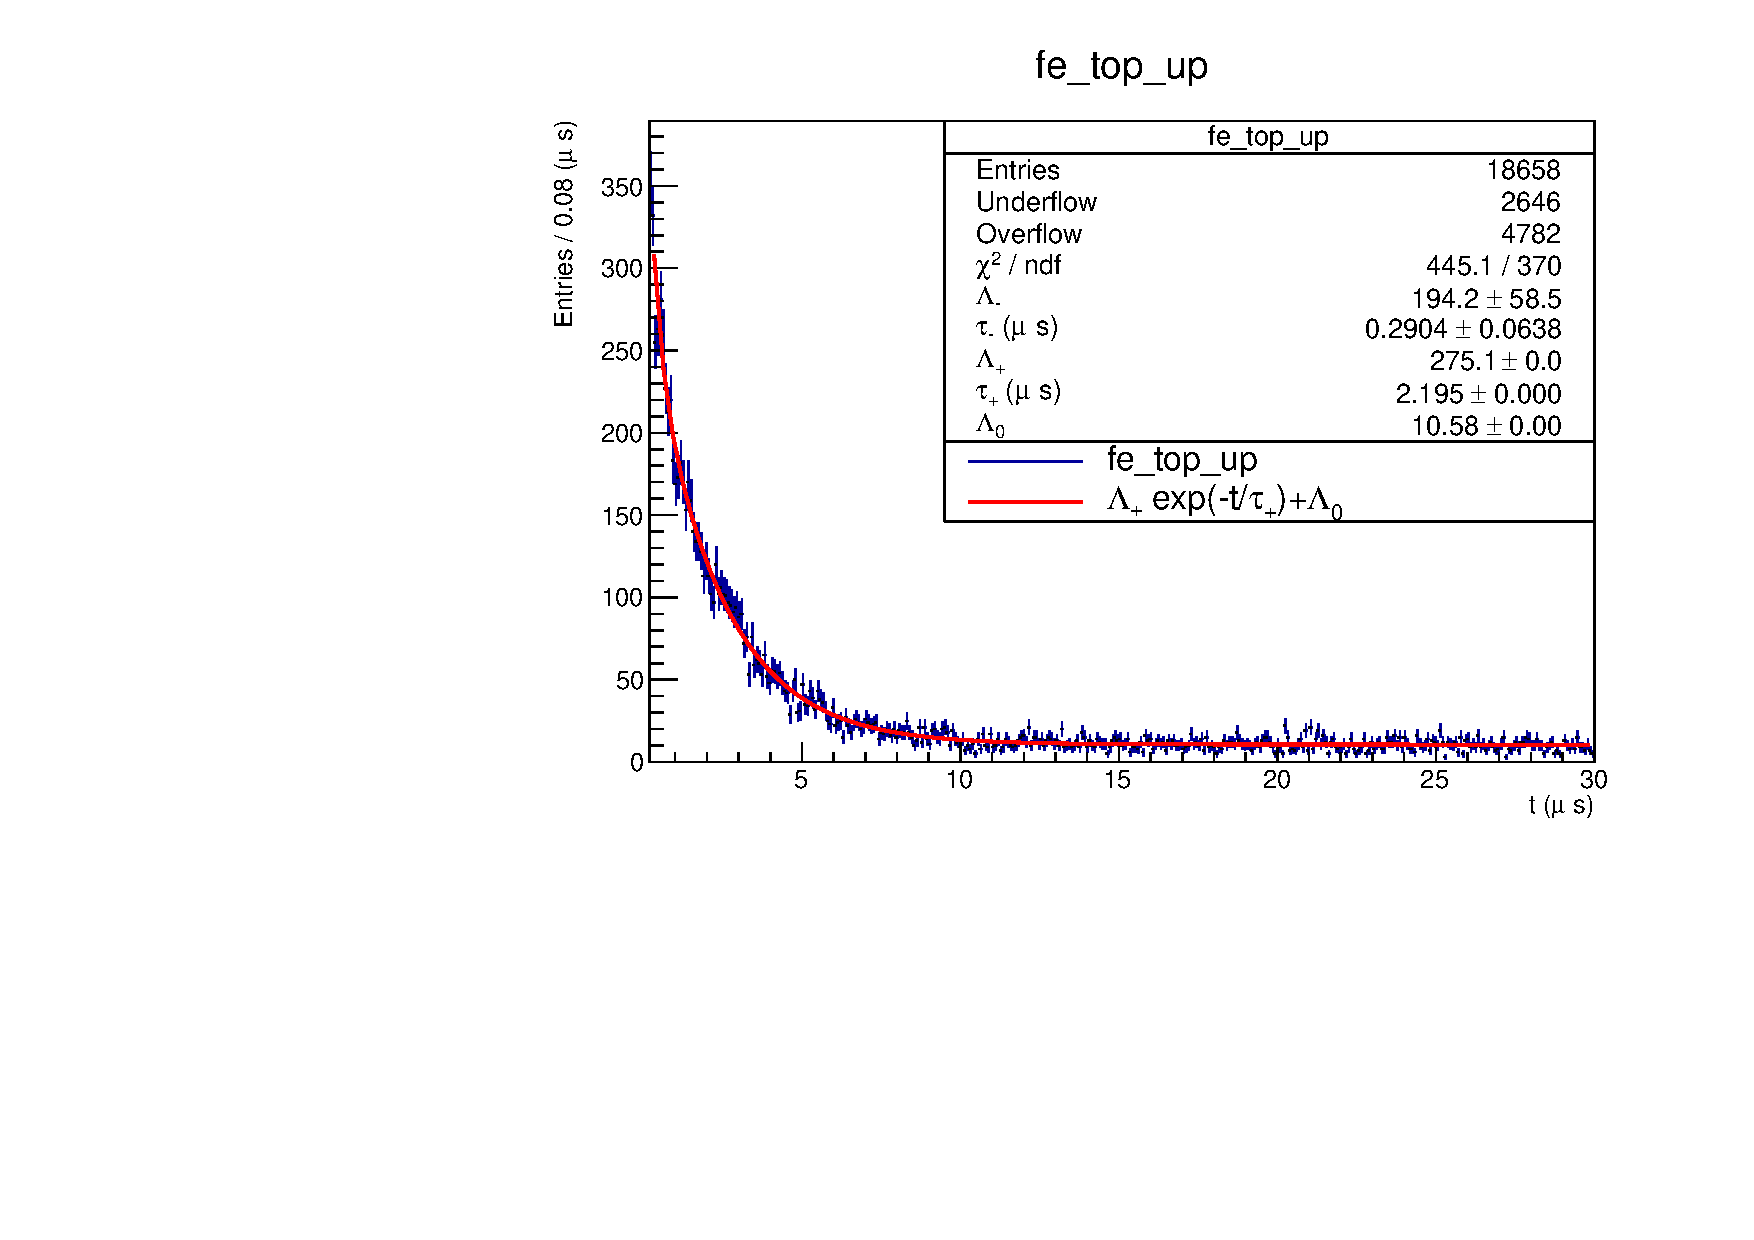
\includegraphics[scale=0.45]{Lab4/Mudecay/fe_top_up.pdf} 
\label{FEUP}
\end{figure}

\begin{figure}[h!]
\centering
\caption{Time distribution of Fe TOP DOWN fitted in the range [0.9, 30] $\mu s$. [10-11-12-17-19-26/05/22]}
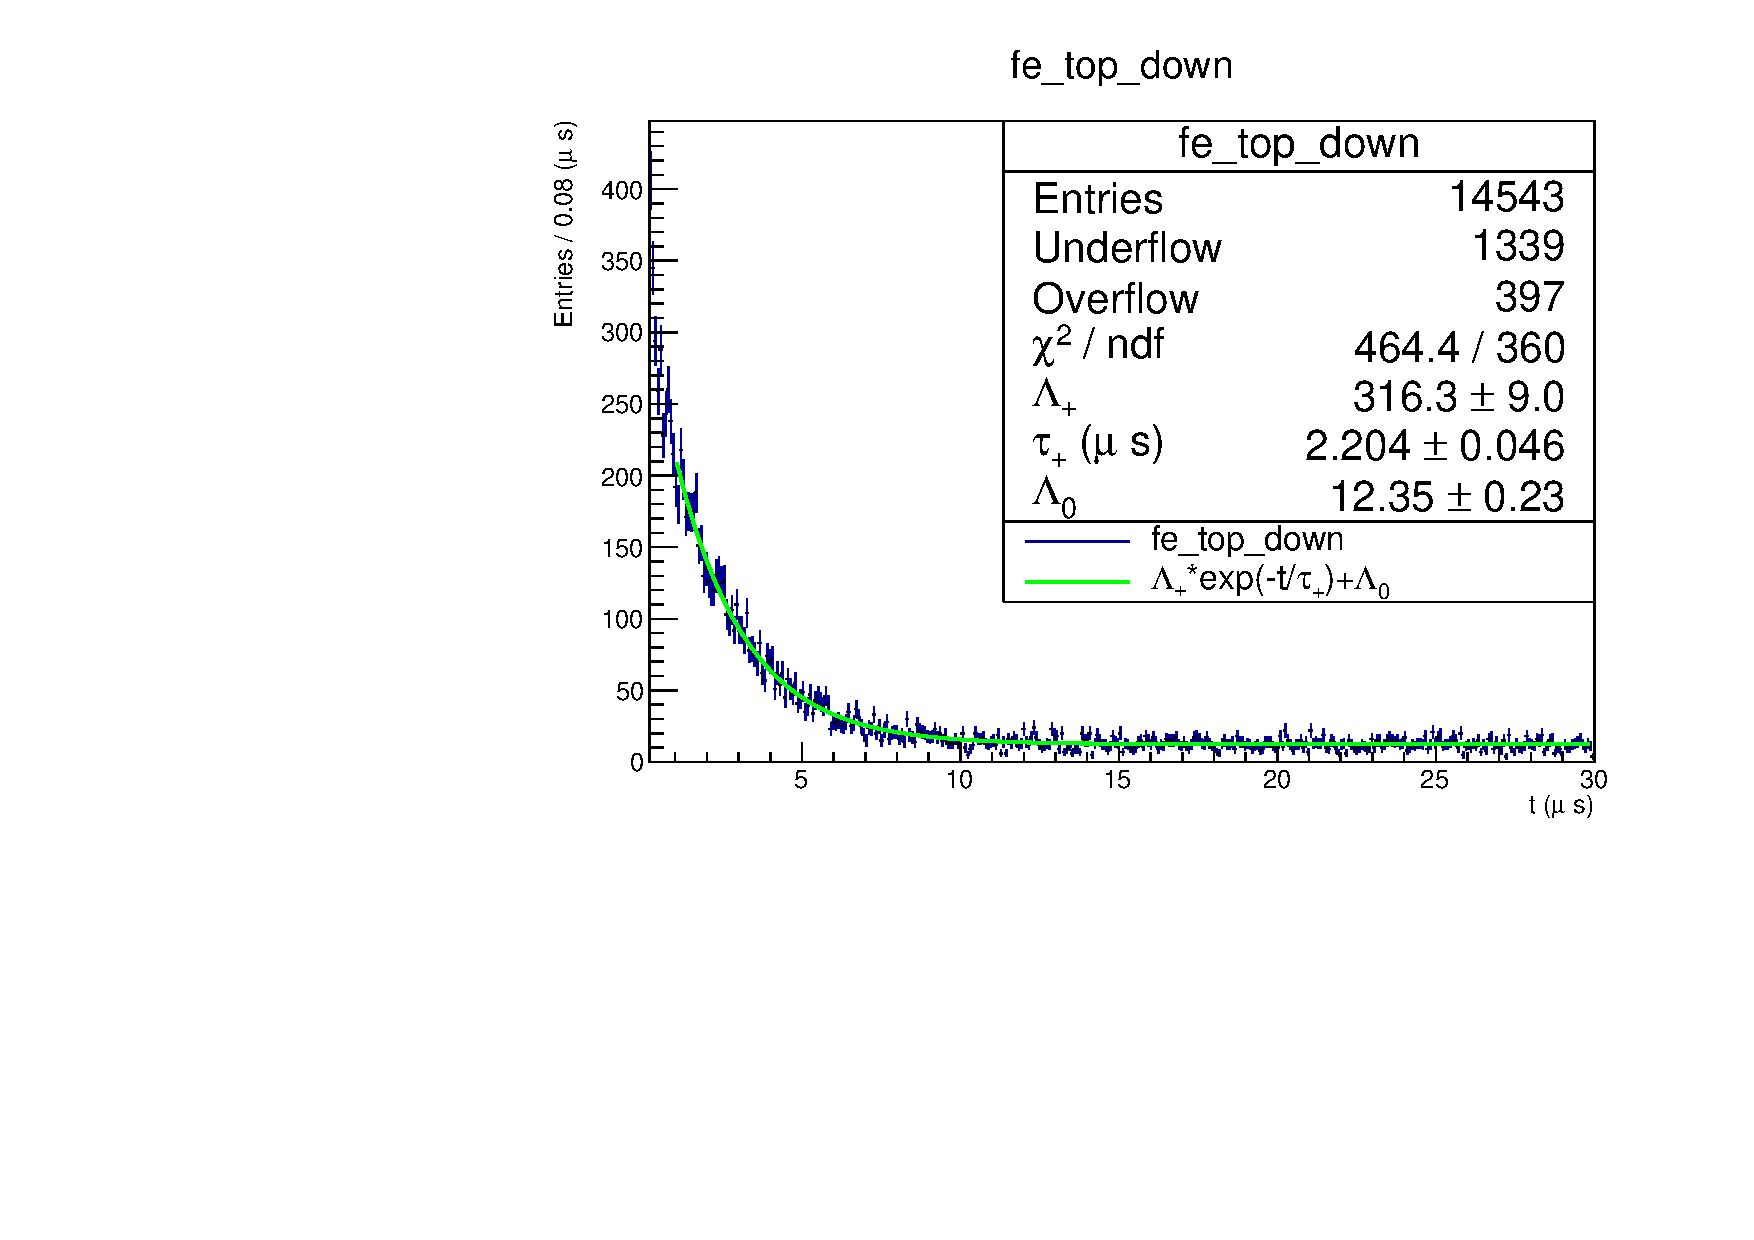
\includegraphics[scale=0.45]{Lab4/Mudecay/fe_top_down.pdf} 
\label{FEDWN}
\end{figure}


The two lifetimes found are compatible within a standard deviation. Since the two sets of data are independent, coming from different scintillators, they can be merged and then fitted once more, as in Figure \ref{FETOT}.

\begin{figure}[h!]
\centering
\caption{Time distribution of Fe TOP TOT fitted in the range [0.9, 30] $\mu s$. In the picture the uncertainty reported for $\tau_+$ is 0.0, while in reality it's 0.03. [10-11-12-17-19-26/05/22]}
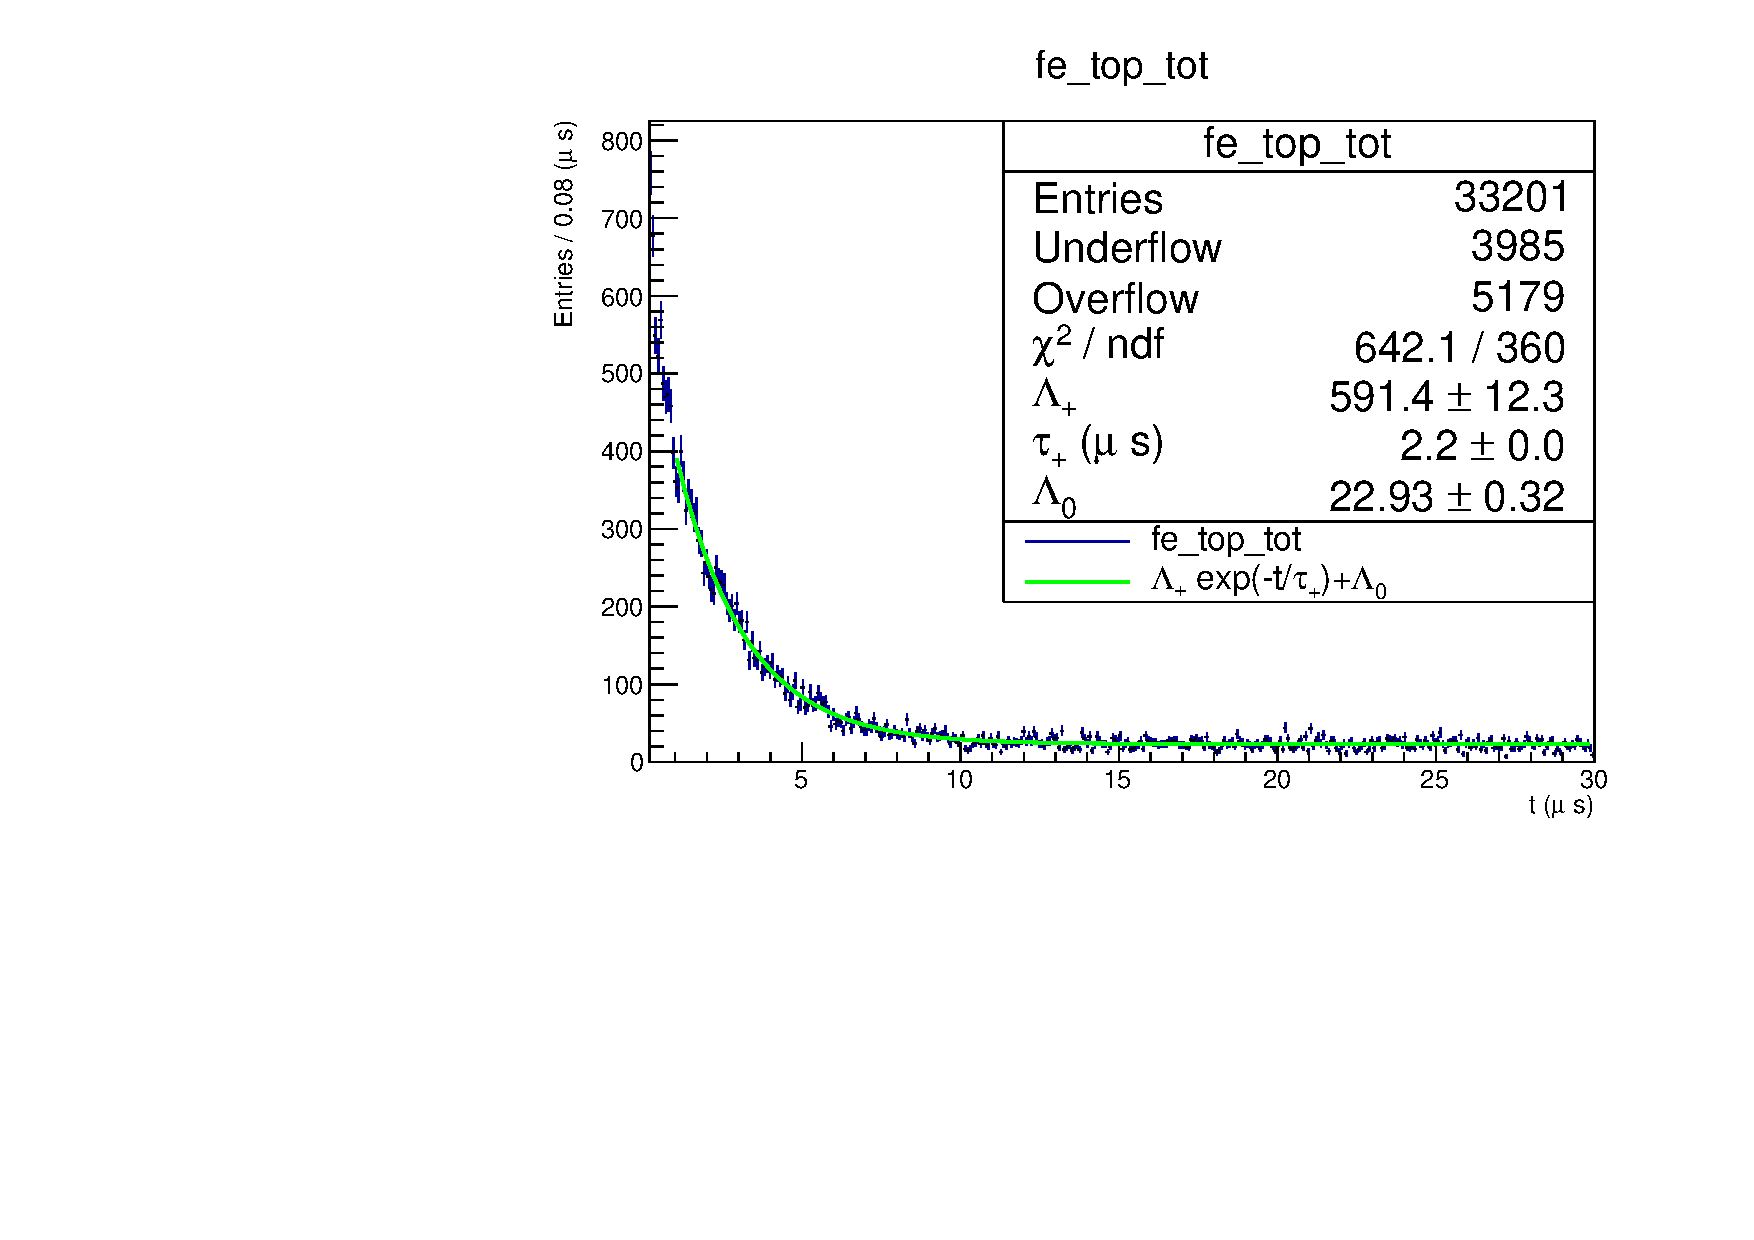
\includegraphics[scale=0.45]{Lab4/Mudecay/fe_top_tot.pdf} 
\label{FETOT}
\end{figure}

The result is $\tau_+=2.20 \pm 0.03 \text{ (stat)}  \pm 0.01 \text{ (syst) }\mu$s. This is compatible with the PDG value reported in Table \ref{mulifetimematerials} within one standard deviation. The goodness of fit is not great at 642/360.









\subsection{$\tau_+$ from Al}

The same procedure can be executed on Al, which was always kept in the BOT slot. An issue present in Al in this regard is that the shorter lifetime is $\sim$0.9 $\mu$s, so we cannot start the fit at 0.9 $\mu$s like we have done for Fe. In Figures \ref{ALUP} and \ref{ALDWN} the two UP and DOWN data sets for Al are fitted with the same model, only this time starting from 2.5 $\mu$s.


\begin{figure}[h!]
\centering
\caption{Time distribution of Al BOT UP fitted in the range [2.5, 30] $\mu s$. [19-26/05/22]}
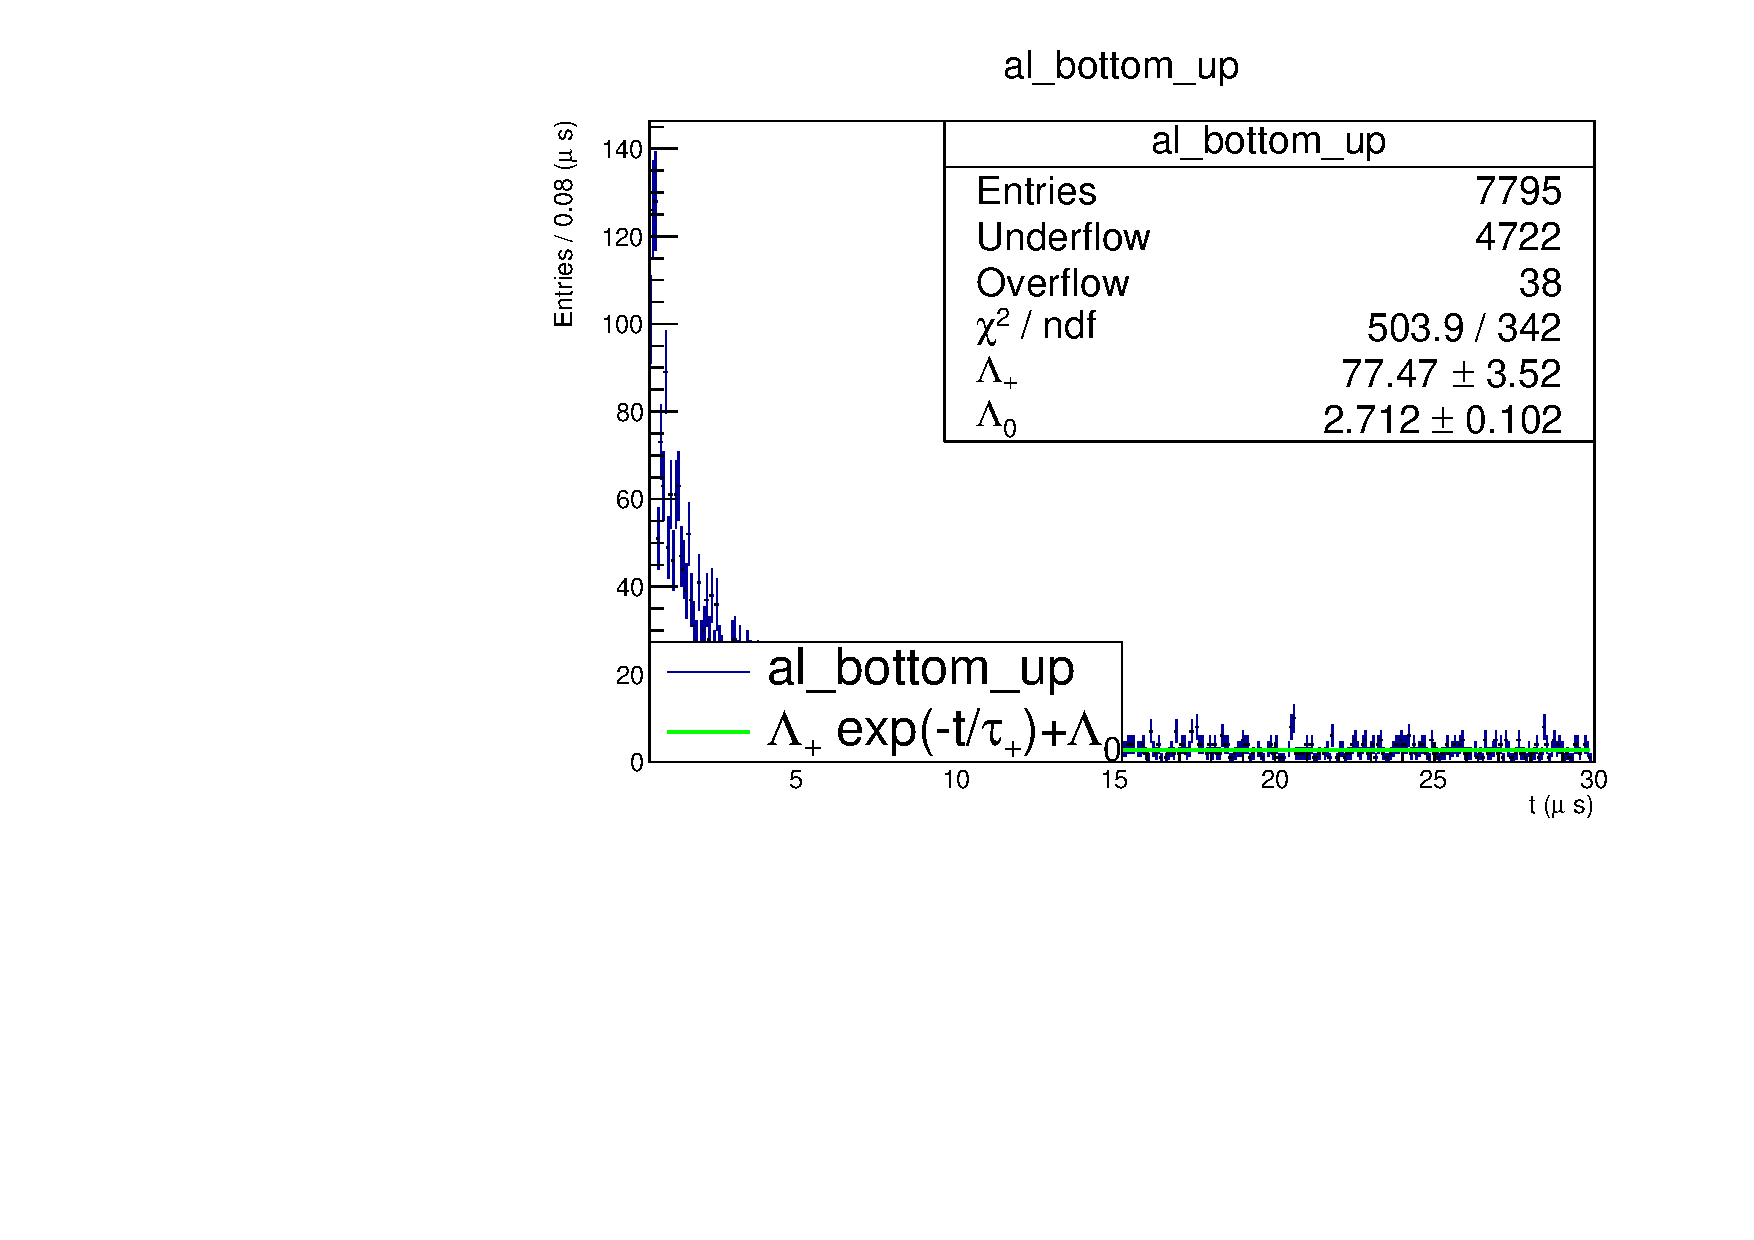
\includegraphics[scale=0.45]{Lab4/Mudecay/al_bottom_up.pdf} 
\label{ALUP}
\end{figure}

\begin{figure}[h!]
\centering
\caption{Time distribution of Al BOT DOWN fitted in the range [2.5, 30] $\mu s$. [19-26/05/22]}
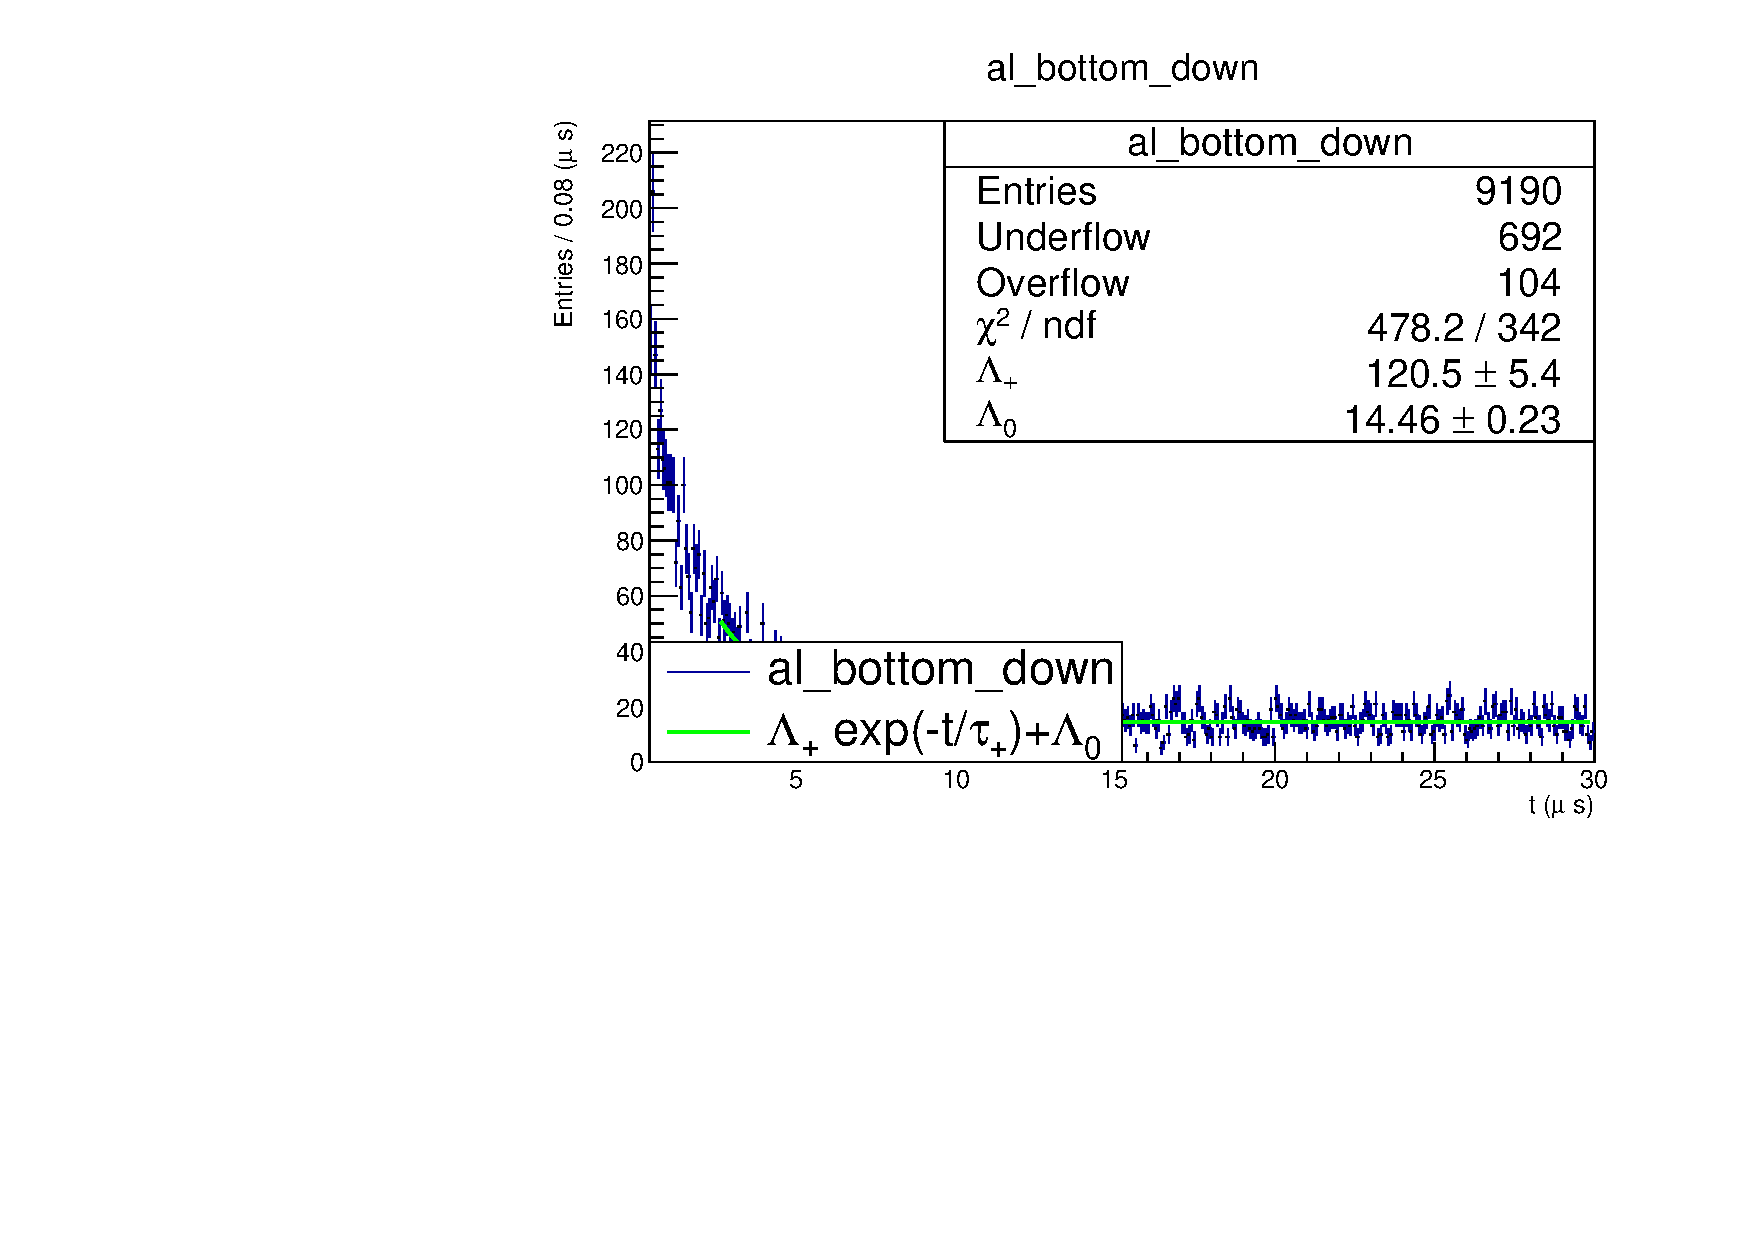
\includegraphics[scale=0.45]{Lab4/Mudecay/al_bottom_down.pdf} 
\label{ALDWN}
\end{figure}


They are found to be compatible within a standard deviation, so the data sets are merged and fitted as per Figure \ref{ALTOT}

\begin{figure}[h!]
\centering
\caption{Time distribution of Al BOT TOT fitted in the range [2.5, 30] $\mu s$. [19-26/05/22]}
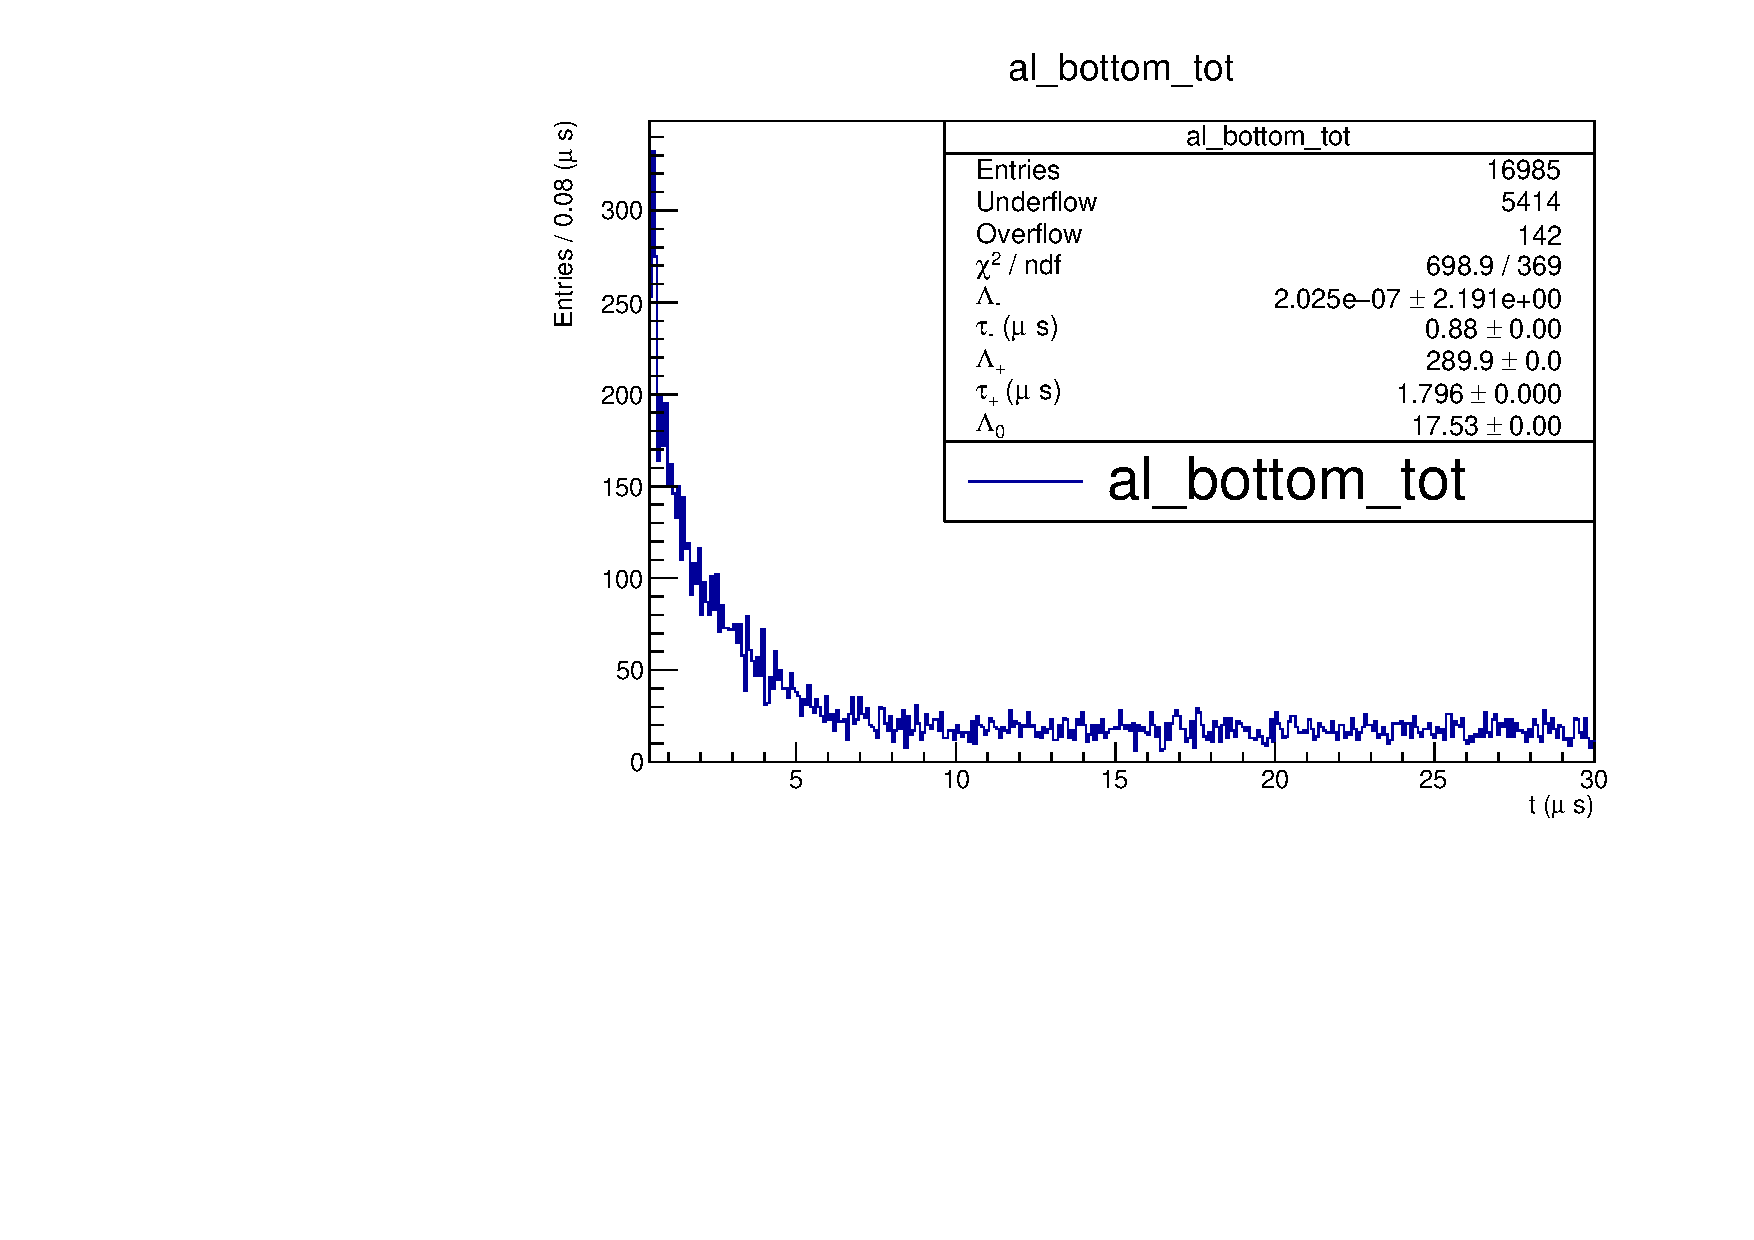
\includegraphics[scale=0.45]{Lab4/Mudecay/al_bottom_tot.pdf} 
\label{ALTOT}
\end{figure}



The result found is $\tau_+=1.80 \pm 0.09 \text{ (stat)} \pm 0.03\text{ (syst) }\mu$s. The statistical uncertainty is greater by a factor of 3 compared to Fe, but not because of a nine fold difference in data acquired (it is actually less than 3 times: 41k vs 17k). The reason is instead that the fit starts at more than a $\tau_+$ lifetime, so the long exponential is already starting to be suppressed compared to the constant background offset. 
%($\chi^2_{free} = 557$ and $\chi^2_{fix} = 574$ )

The result is 4 standard deviations from the expected value. This isn't due to the presence of $\tau_-$ because if the fit is started at e.g. 4 $\mu$s the value found for $\tau_+$ with single exponential fit is $1.7 \pm 0.2 \text{ (stat) } \pm 0.2\text{ (syst) }\mu$s. This is still more than two standard deviations from the expected value and is measured in a region where the short exponential is already suppressed by a factor of more than 50.

\\


\subsection{$\tau_+$ from PbAl}

The same reasoning can be applied when using as material a slab made of Pb with a thin layer of Al on the outside (Figures \ref{PBALUP} and \ref{PBALDWN}). 

\begin{figure}[h!]
\centering
\caption{Time distribution of Pb Al BOT UP fitted in the range [3.5, 30] $\mu s$. [12-17/05/22]}
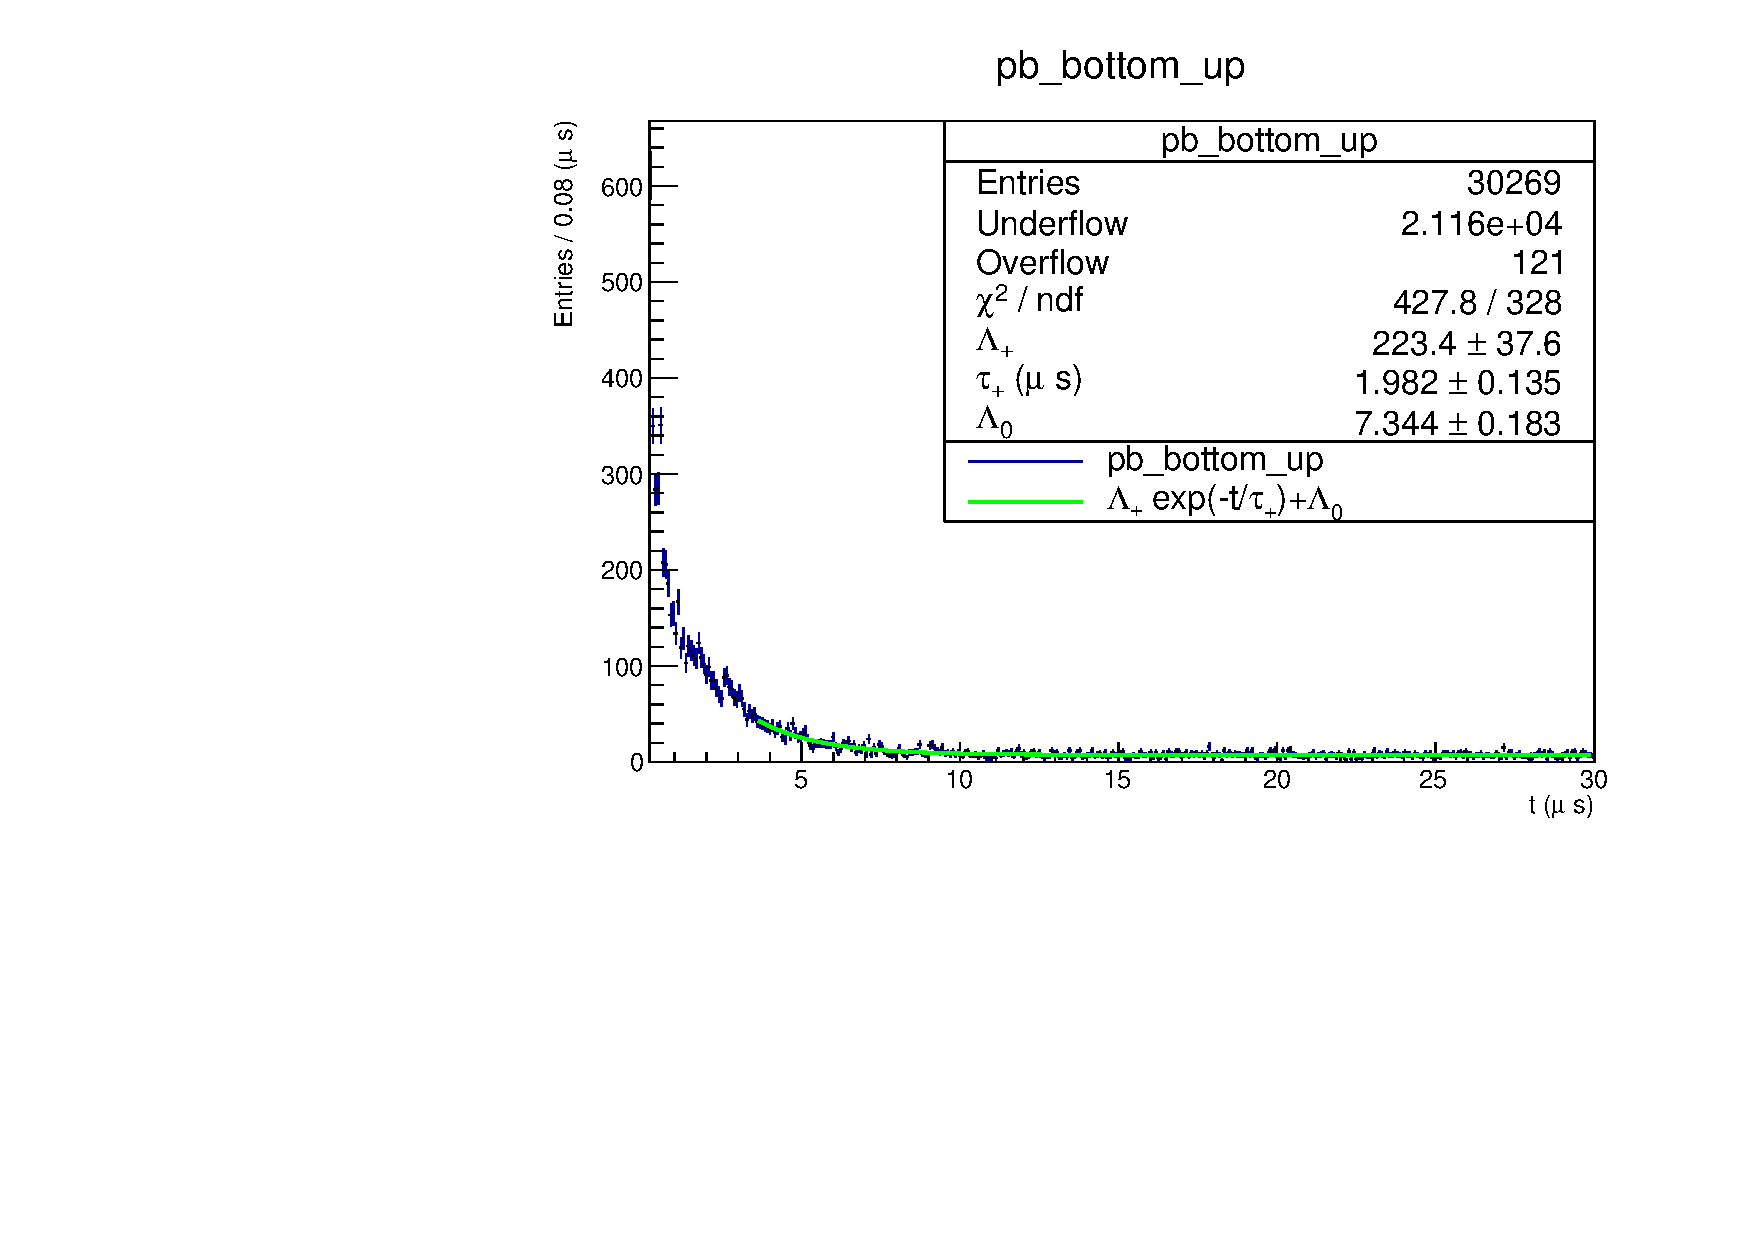
\includegraphics[scale=0.45]{Lab4/Mudecay/pb_bottom_up.pdf} 
\label{PBALUP}
\end{figure}

\begin{figure}[h!]
\centering
\caption{Time distribution of Pb Al BOT DOWN fitted in the range [3.5, 30] $\mu s$. [12-17/05/22]}
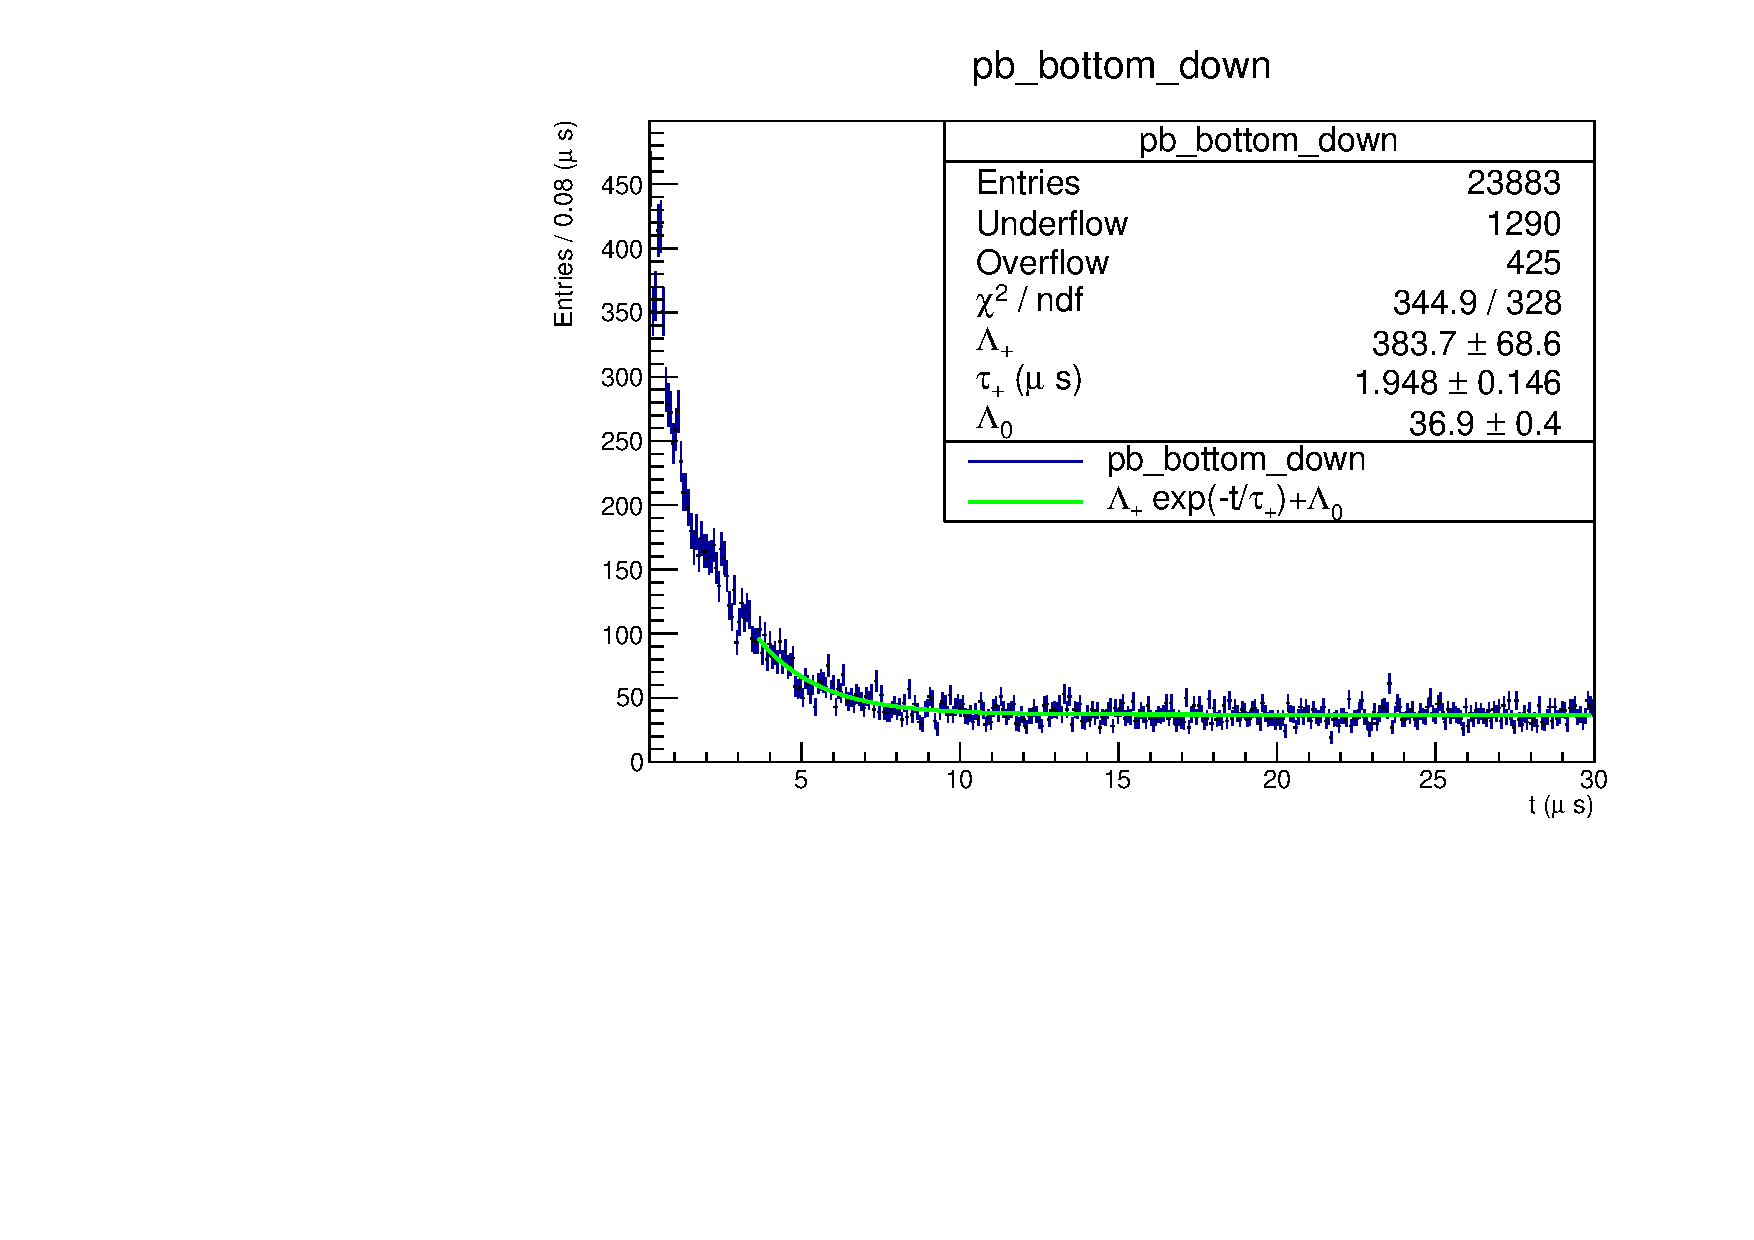
\includegraphics[scale=0.45]{Lab4/Mudecay/pb_bottom_down.pdf} 
\label{PBALDWN}
\end{figure}


They are found to be compatible within a standard deviation, so the data sets are merged and fitted. The total data when fitted in the range between 3.5 $\mu s$ and 30 $\mu s$ give (Figure \ref{PBALTOT}) $\tau_+=2.0 \pm 0.1 \text{ (stat)} \pm 0.1 \text{ (syst) }\mu$s. This result is compatible with the expected value within one standard deviation. 

\begin{figure}[h!]
\centering
\caption{Time distribution of Pb Al BOT TOT fitted in the range [3.5, 30] $\mu s$. [12-17/05/22]}
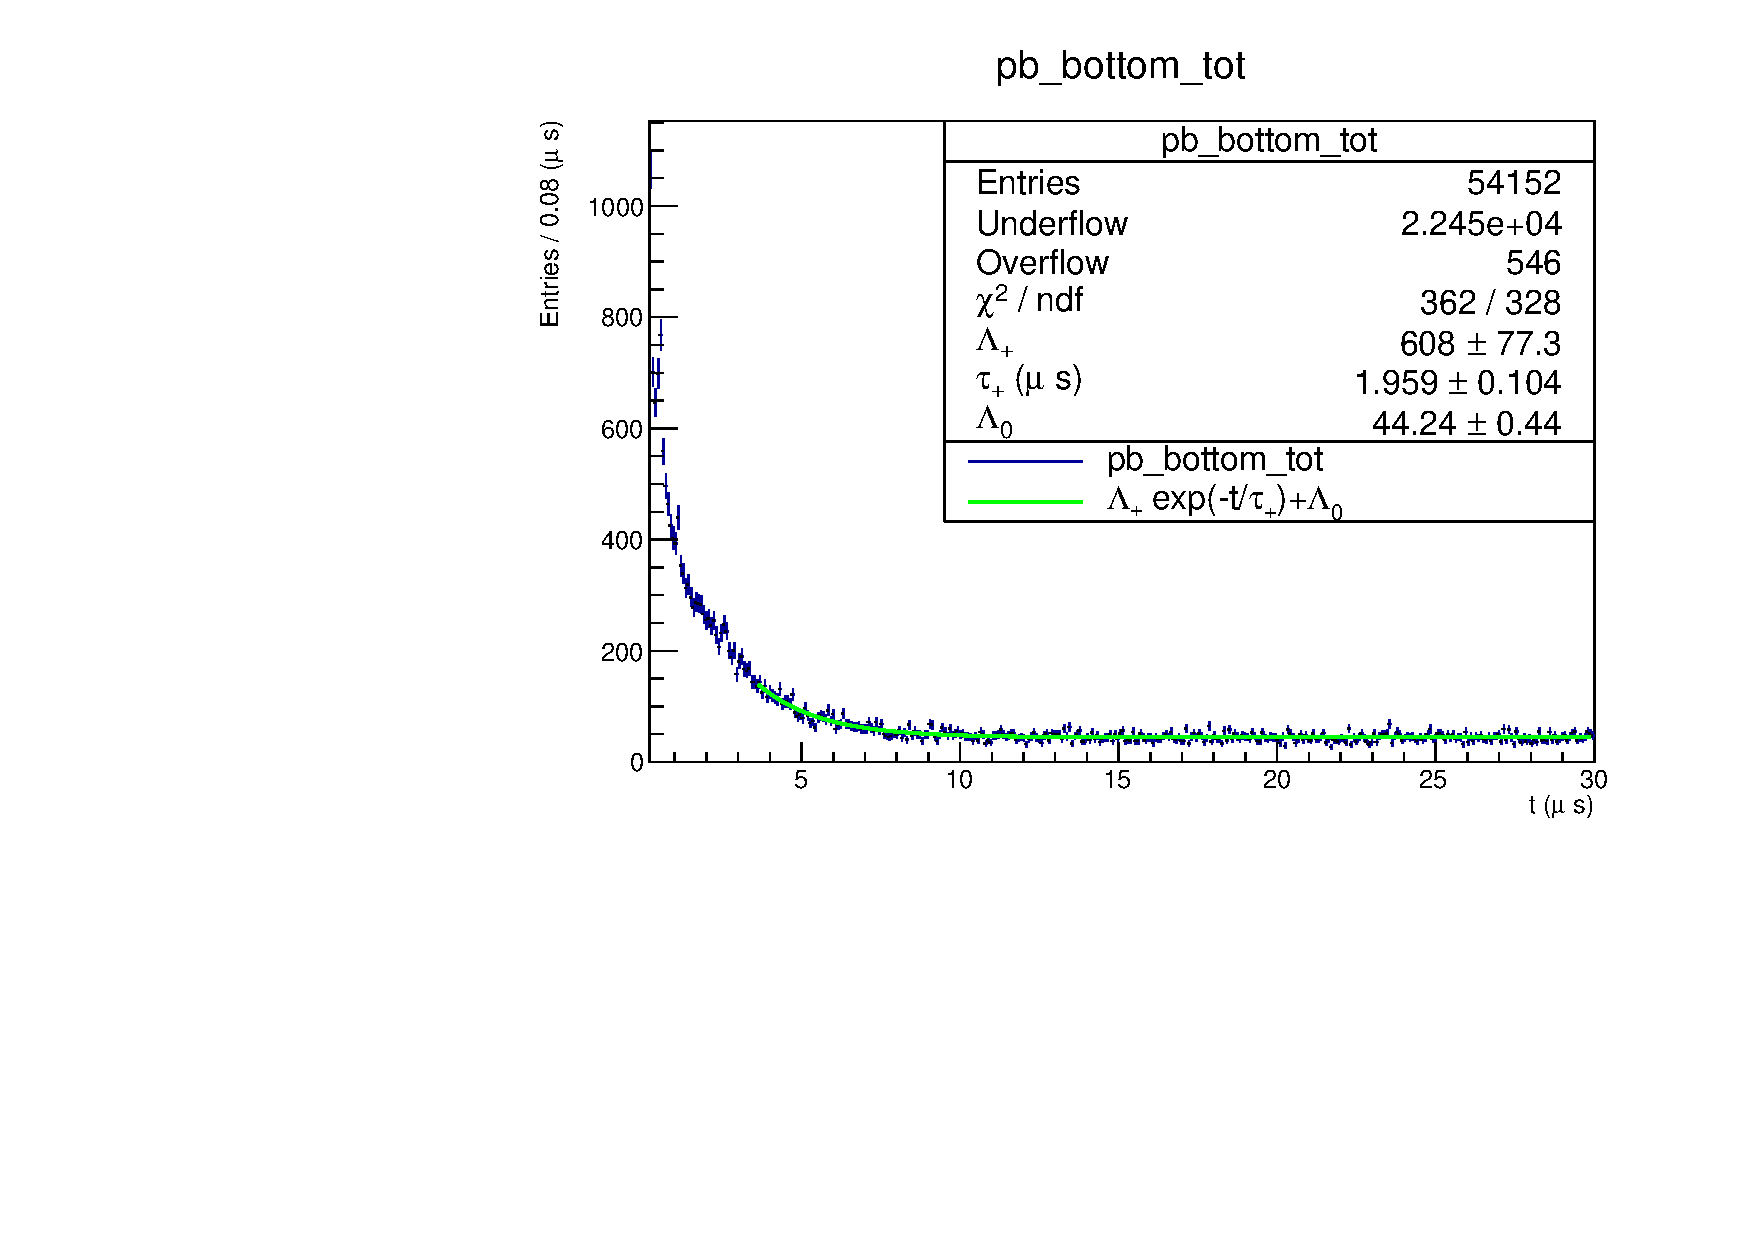
\includegraphics[scale=0.45]{Lab4/Mudecay/pb_bottom_tot.pdf} 
\label{PBALTOT}
\end{figure}



\subsection{$\tau_+$ from NaCl}


Analogously, boxes of NaCl \footnote{9 boxes 5 cm thick} were used both in the TOP and BOT section of the apparatus (Figure \ref{NACLTOPUP} \ref{NACLTOPDW} \ref{NACLBOTUP} \ref{NACLBOTDW}).

\begin{figure}[h!]
\centering
\caption{Time distribution of NaCl TOP UP fitted in the range [3, 30] $\mu s$. [18-19-24/05/22]}
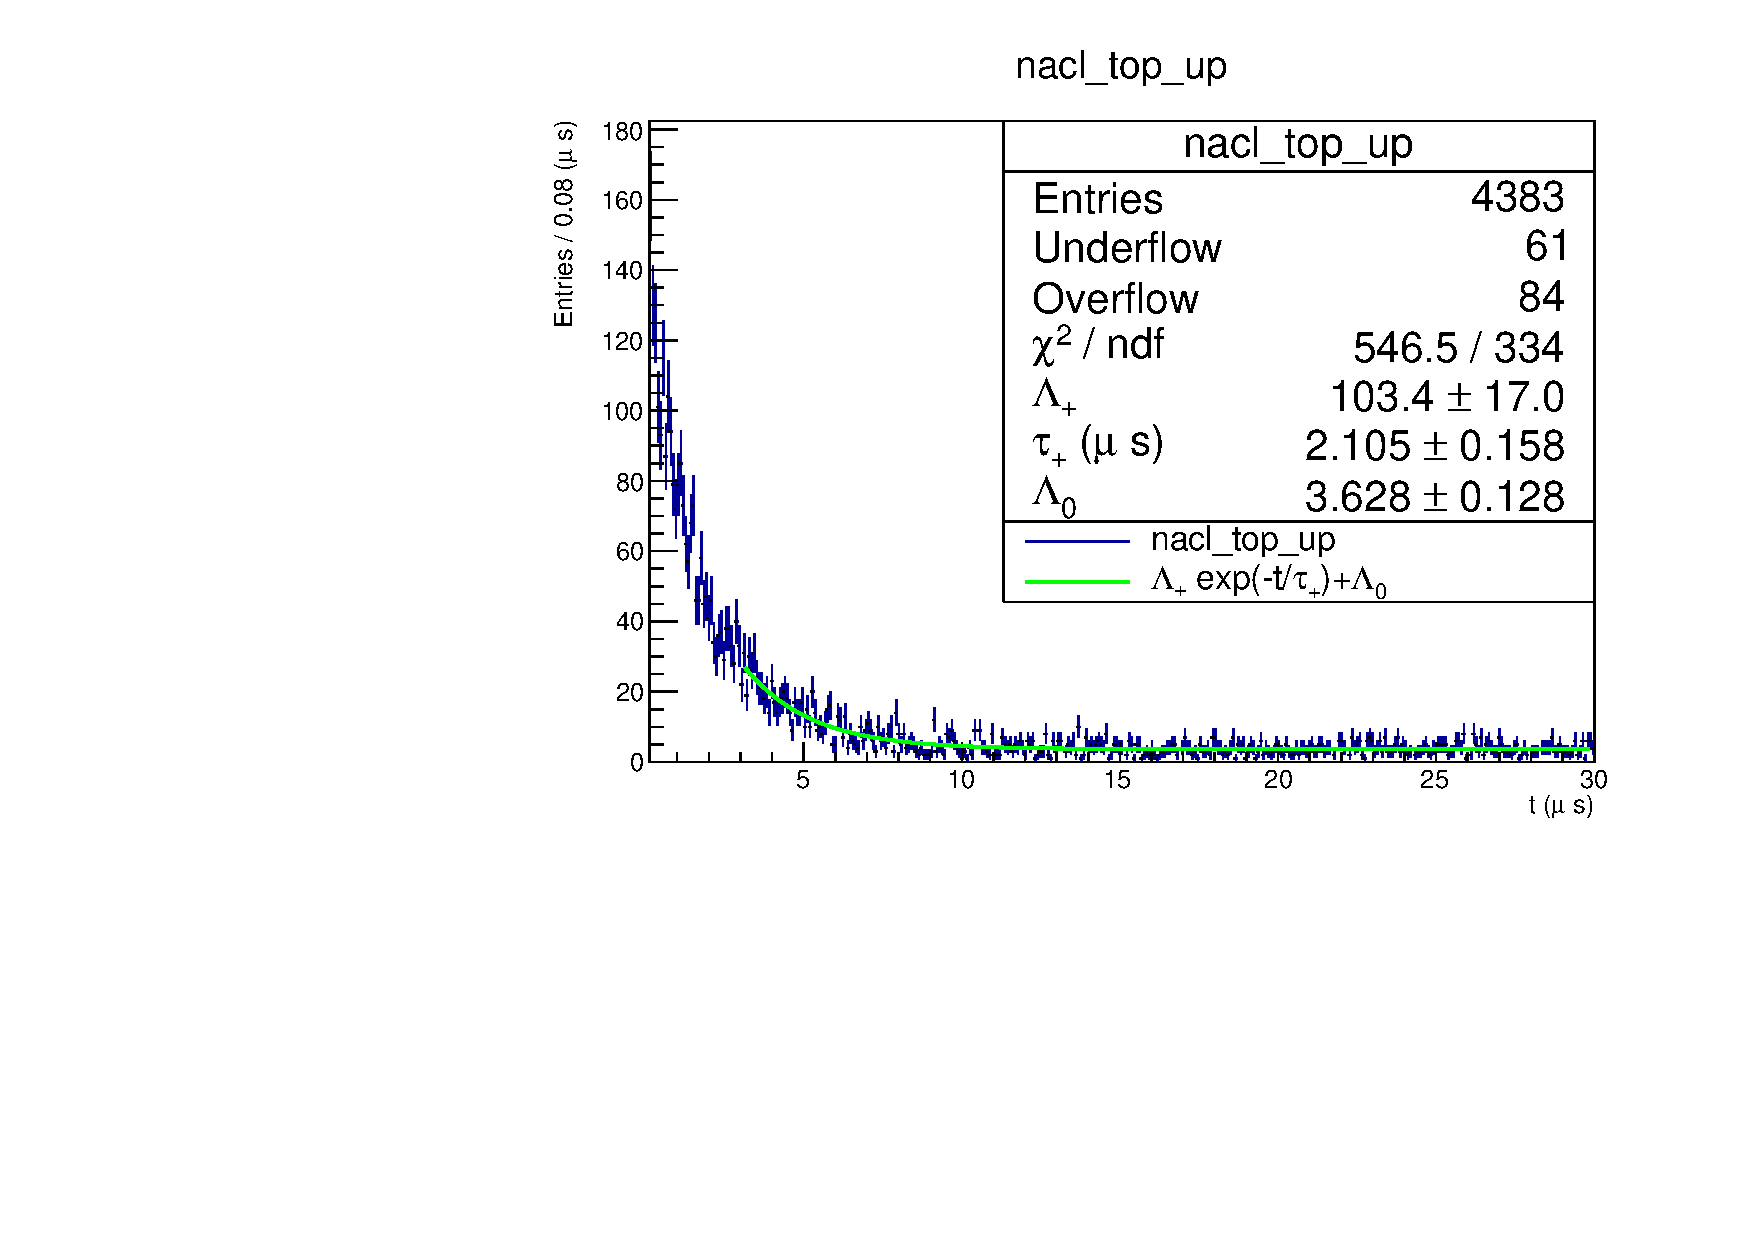
\includegraphics[scale=0.45]{Lab4/Mudecay/nacl_top_up.pdf} 
\label{NACLTOPUP}
\end{figure}

\begin{figure}[h!]
\centering
\caption{Time distribution of NaCl TOP DOWN fitted in the range [3, 30] $\mu s$. [18-19-24/05/22]}
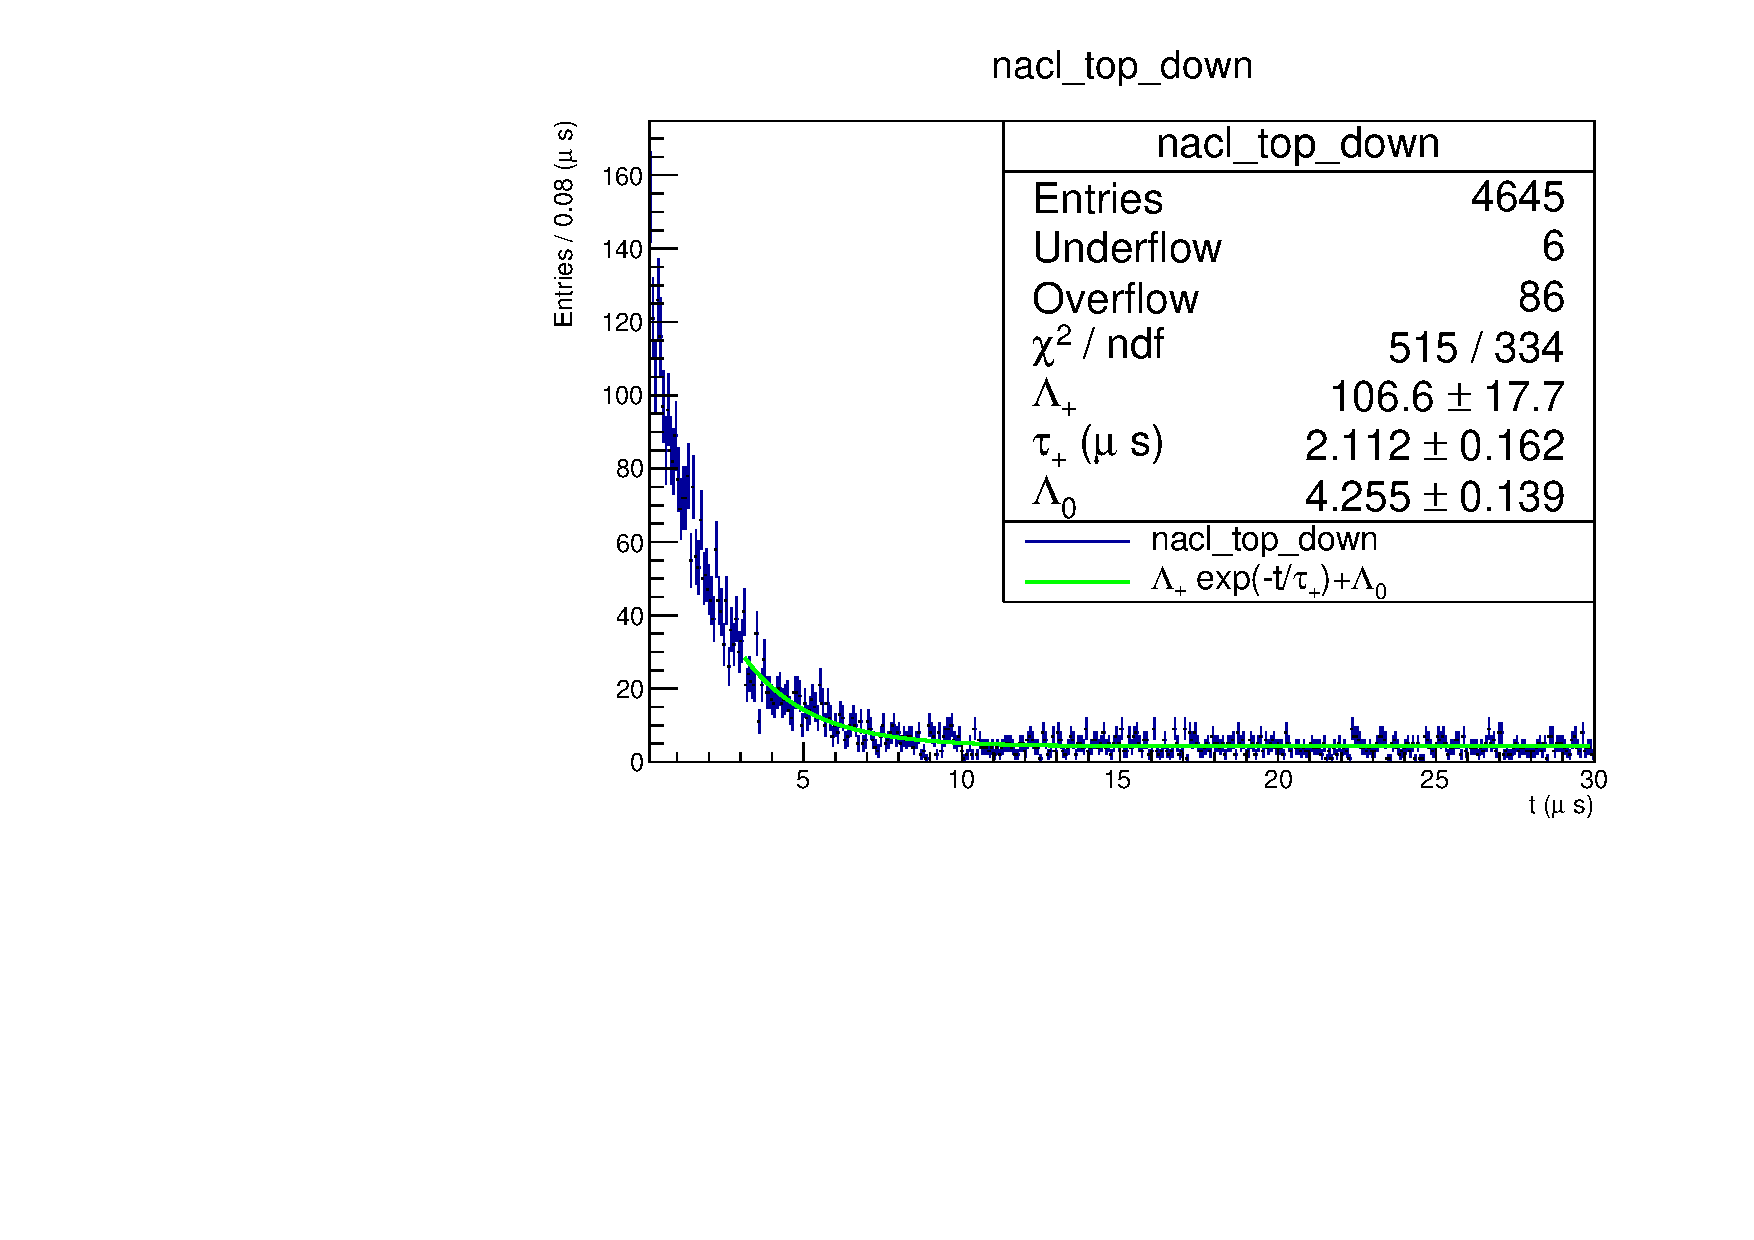
\includegraphics[scale=0.45]{Lab4/Mudecay/nacl_top_down.pdf}
\label{NACLTOPDW}
\end{figure}

\begin{figure}[h!]
\centering
\caption{Time distribution of NaCl BOT UP fitted in the range [3, 30] $\mu s$. [25-26-30/05/22]}
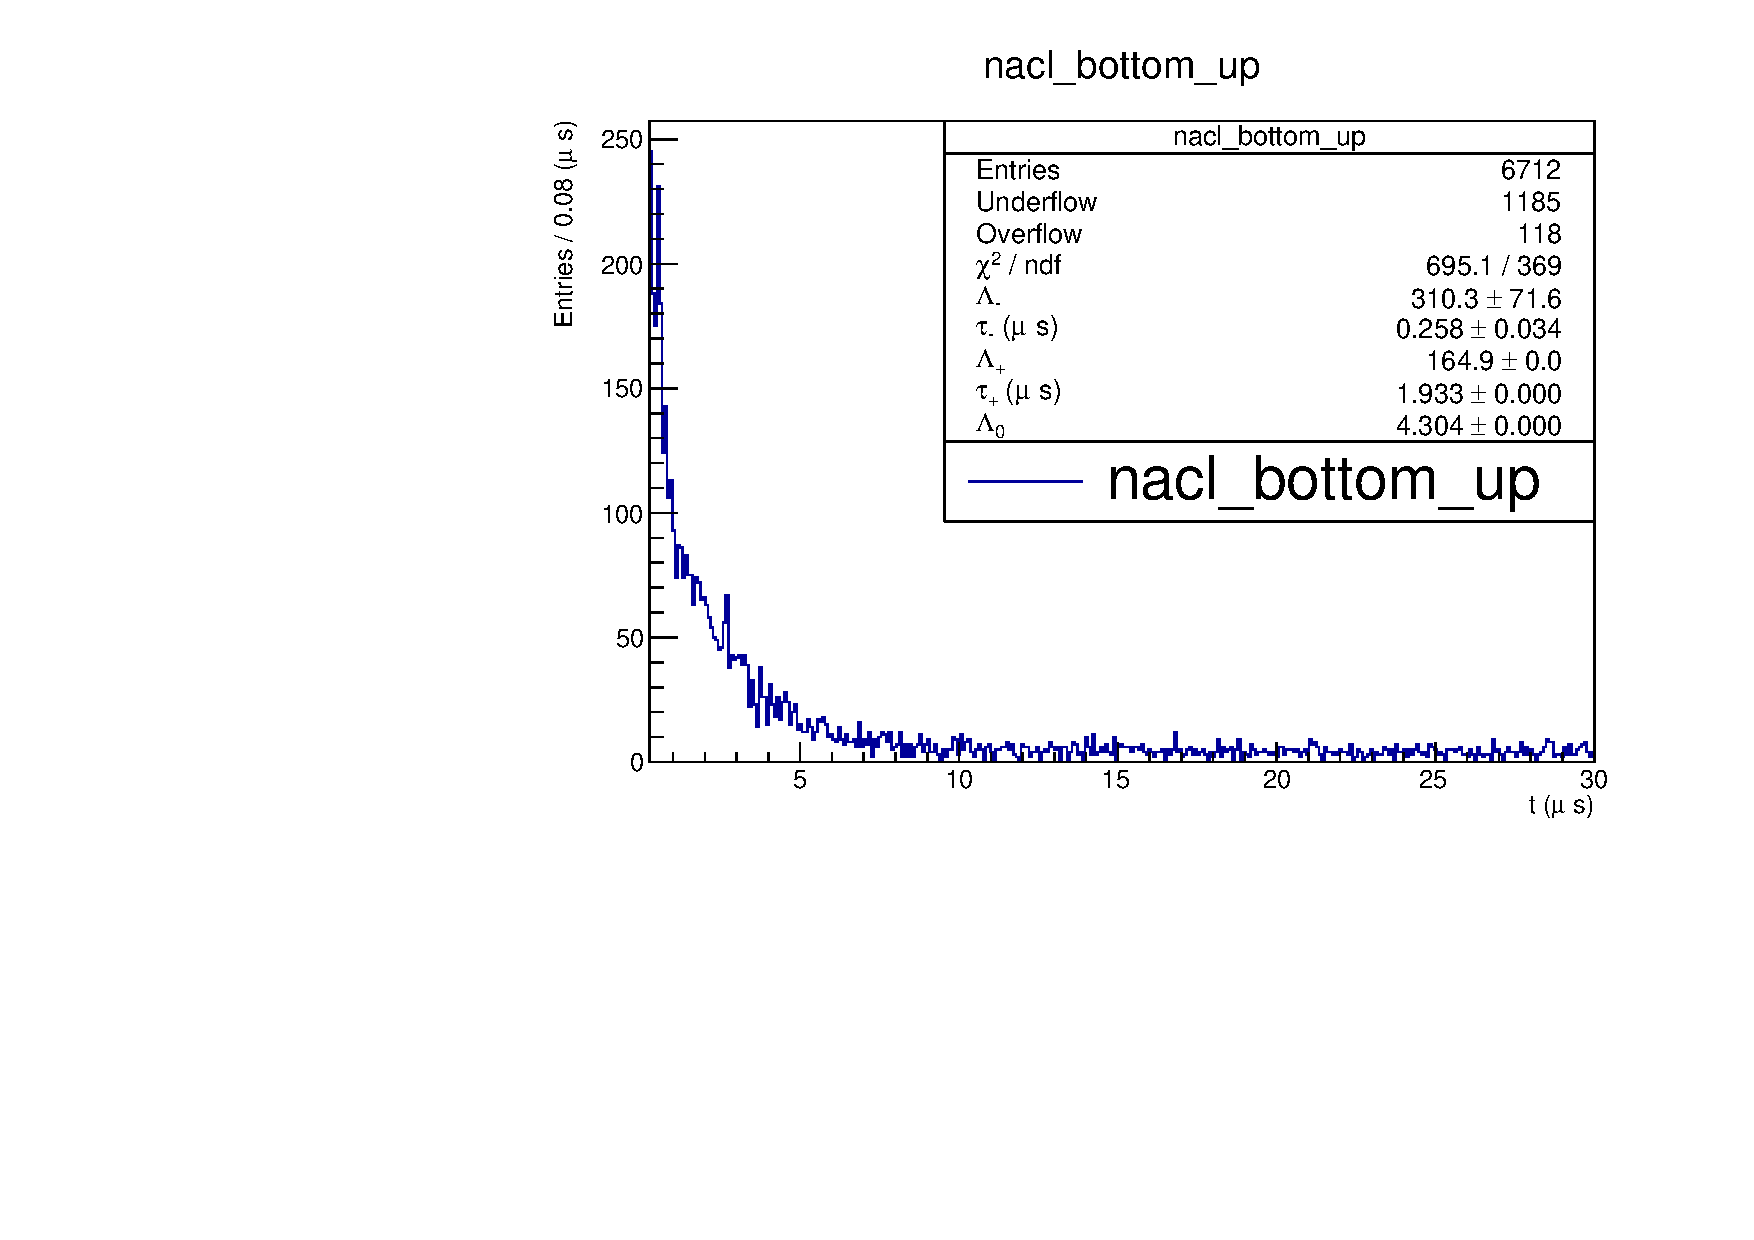
\includegraphics[scale=0.45]{Lab4/Mudecay/nacl_bottom_up.pdf} 
\label{NACLBOTUP}
\end{figure}

\begin{figure}[h!]
\centering
\caption{Time distribution of NaCl BOT DOWN fitted in the range [3, 30] $\mu s$. [25-26-30/05/22]}
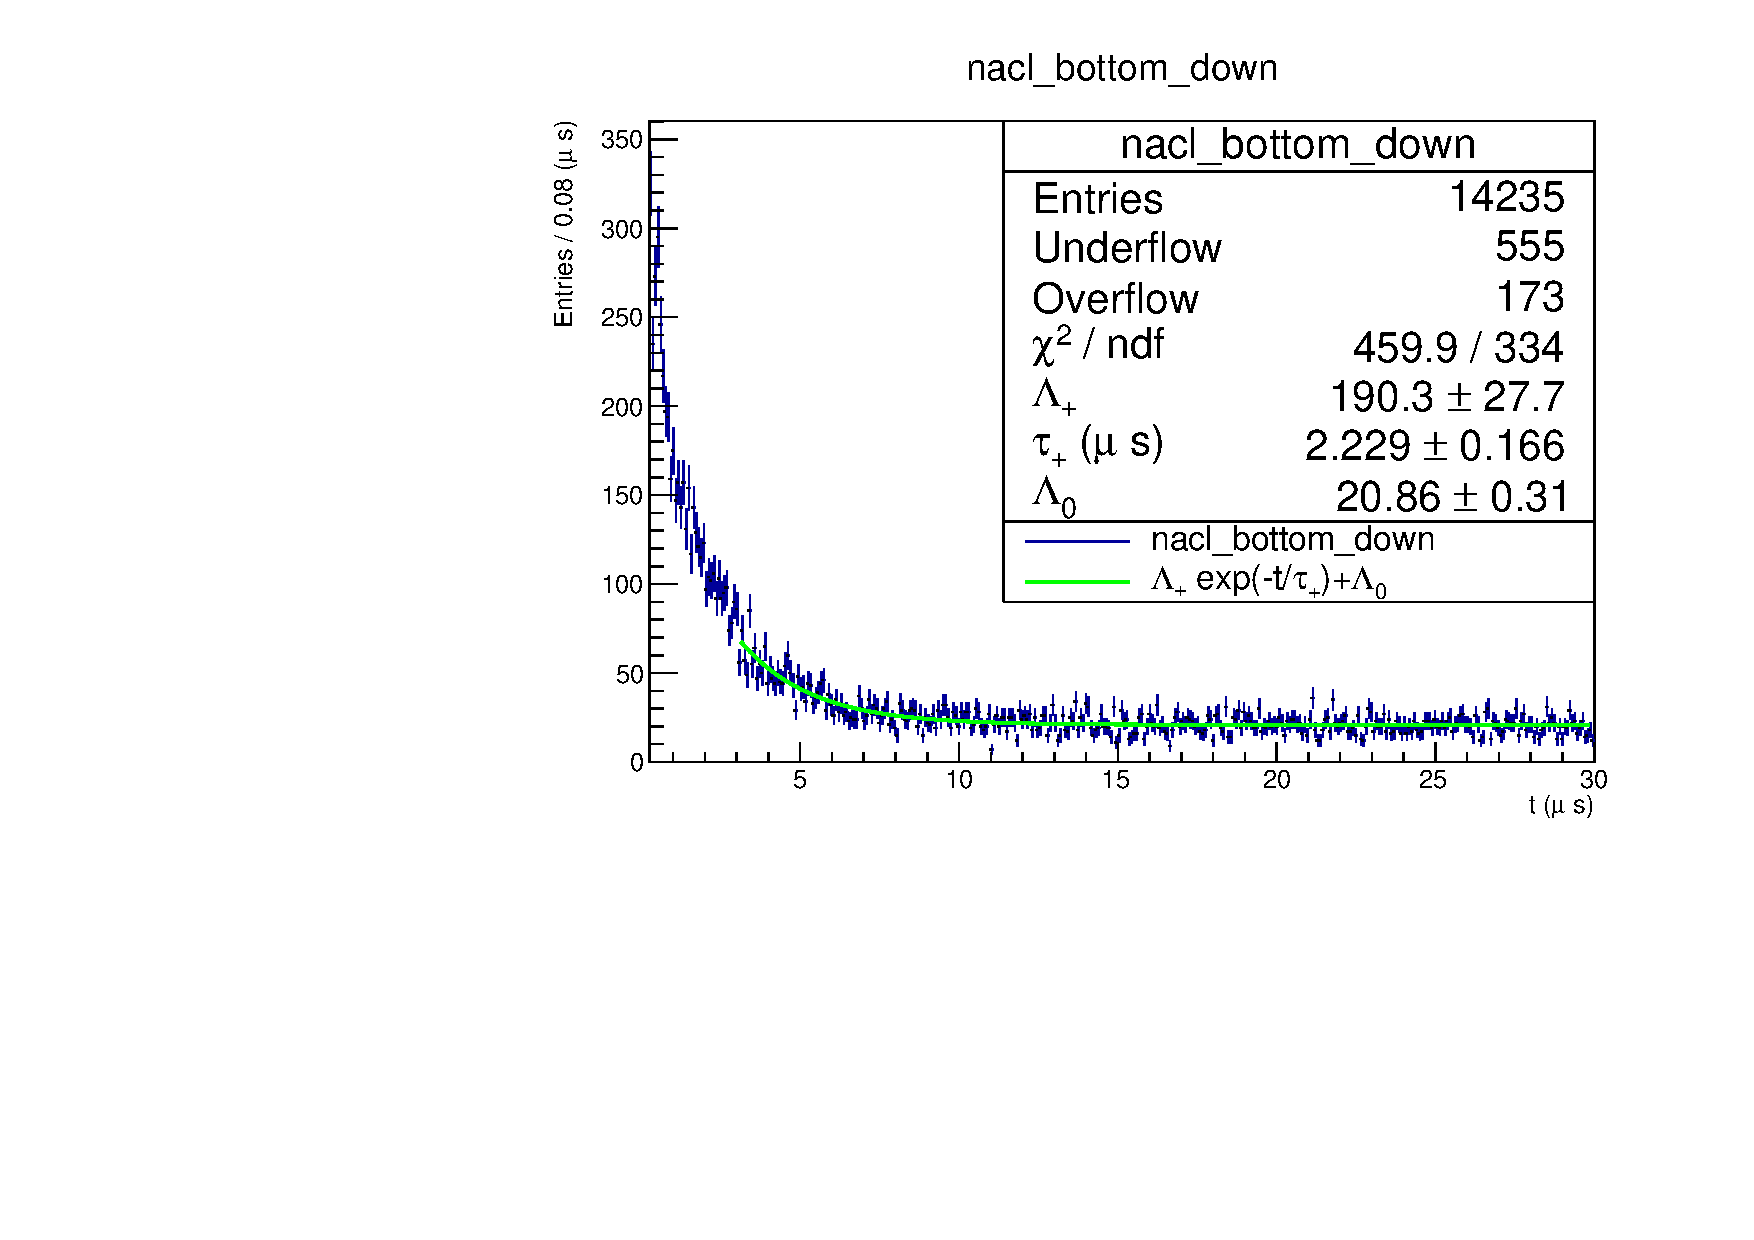
\includegraphics[scale=0.45]{Lab4/Mudecay/nacl_bottom_down.pdf} 
\label{NACLBOTDW}
\end{figure}


Since the UP and DOWN of each section are compatible with each other and are independent (different scintillators), they are merged and fitted from 3 $\mu s$ to 30 $\mu s$ as shown in Figure \ref{NACLTOP} \ref{NACLBOT}.

\begin{figure}[h!]
\centering
\caption{Time distribution of NaCl TOP TOT fitted in the range [3, 30] $\mu s$. [18-19-24/05/22]}
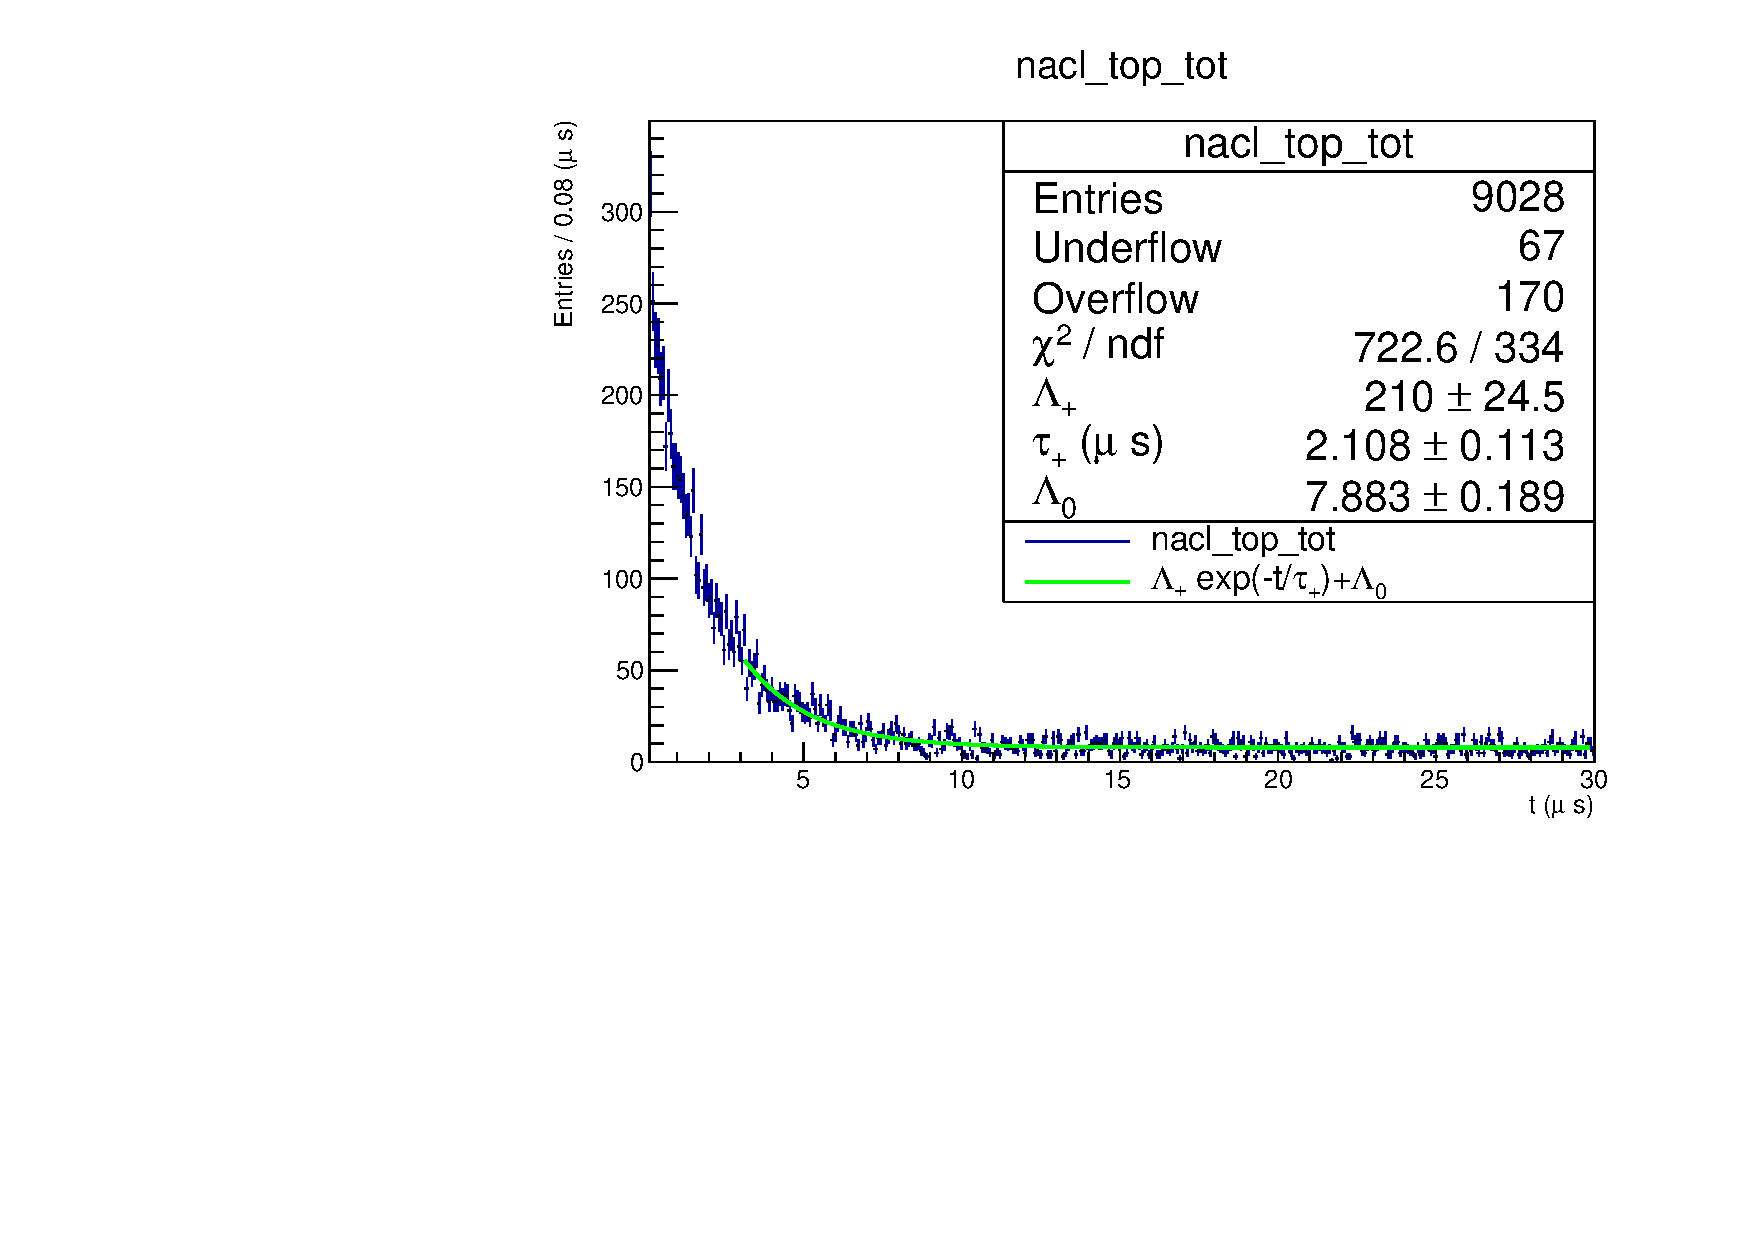
\includegraphics[scale=0.45]{Lab4/Mudecay/nacl_top_tot.pdf}
\label{NACLTOP}
\end{figure}


\begin{figure}[h!]
\centering
\caption{Time distribution of NaCl BOT TOT fitted in the range [3, 30] $\mu s$. [25-26-30/05/22]}
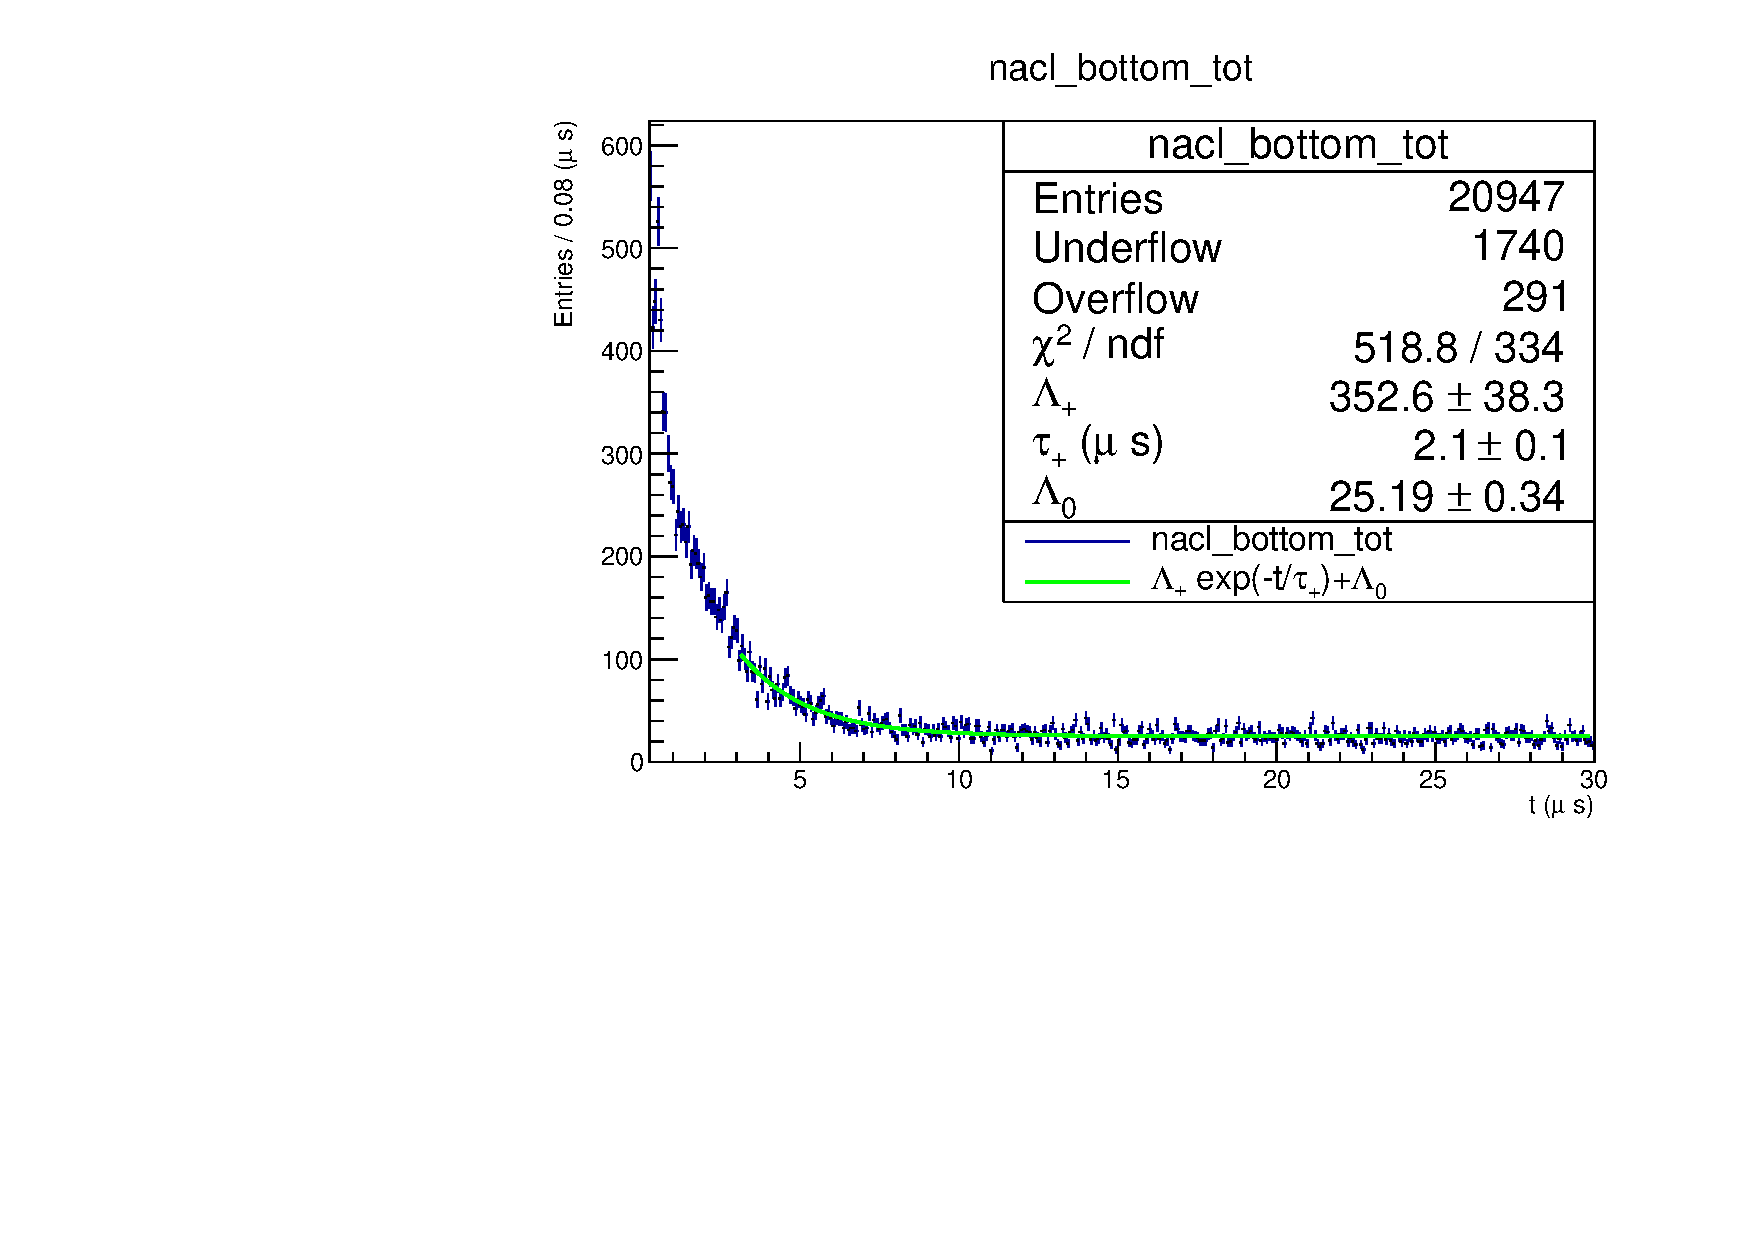
\includegraphics[scale=0.45]{Lab4/Mudecay/nacl_bottom_tot.pdf}
\label{NACLBOT}
\end{figure}



The fits yield  $\tau_+^{TOP}=2.11 \pm 0.11 \text{ (stat)} \pm 0.04 \text{ (syst) }\mu$s and $\tau_+^{BOT}=2.1 \pm 0.1 \text{ (stat)} \pm 0.1 \text{ (syst) }\mu$s. The results are compatible within one standard deviation with the expected value.
%( total $\tau_+=2.11 \pm 0.08 \text{ (stat)} \pm 0.1 \text{ (syst) }\mu$s.) 

\subsection{$\tau_+$ from Mag Fe}

The magnetic circuit schematized in Figure \ref{magnetizedFe} is used in the TOP and BOT sections (Figure \ref{MAGTOPUP} \ref{MAGTOPDW} \ref{MAGBOTUP} \ref{MAGBOTDW}). 

\begin{figure}[h!]
\centering
\caption{Time distribution of Mag Fe TOP UP fitted in the range [1, 30] $\mu s$. [25-26-30/05/22]}
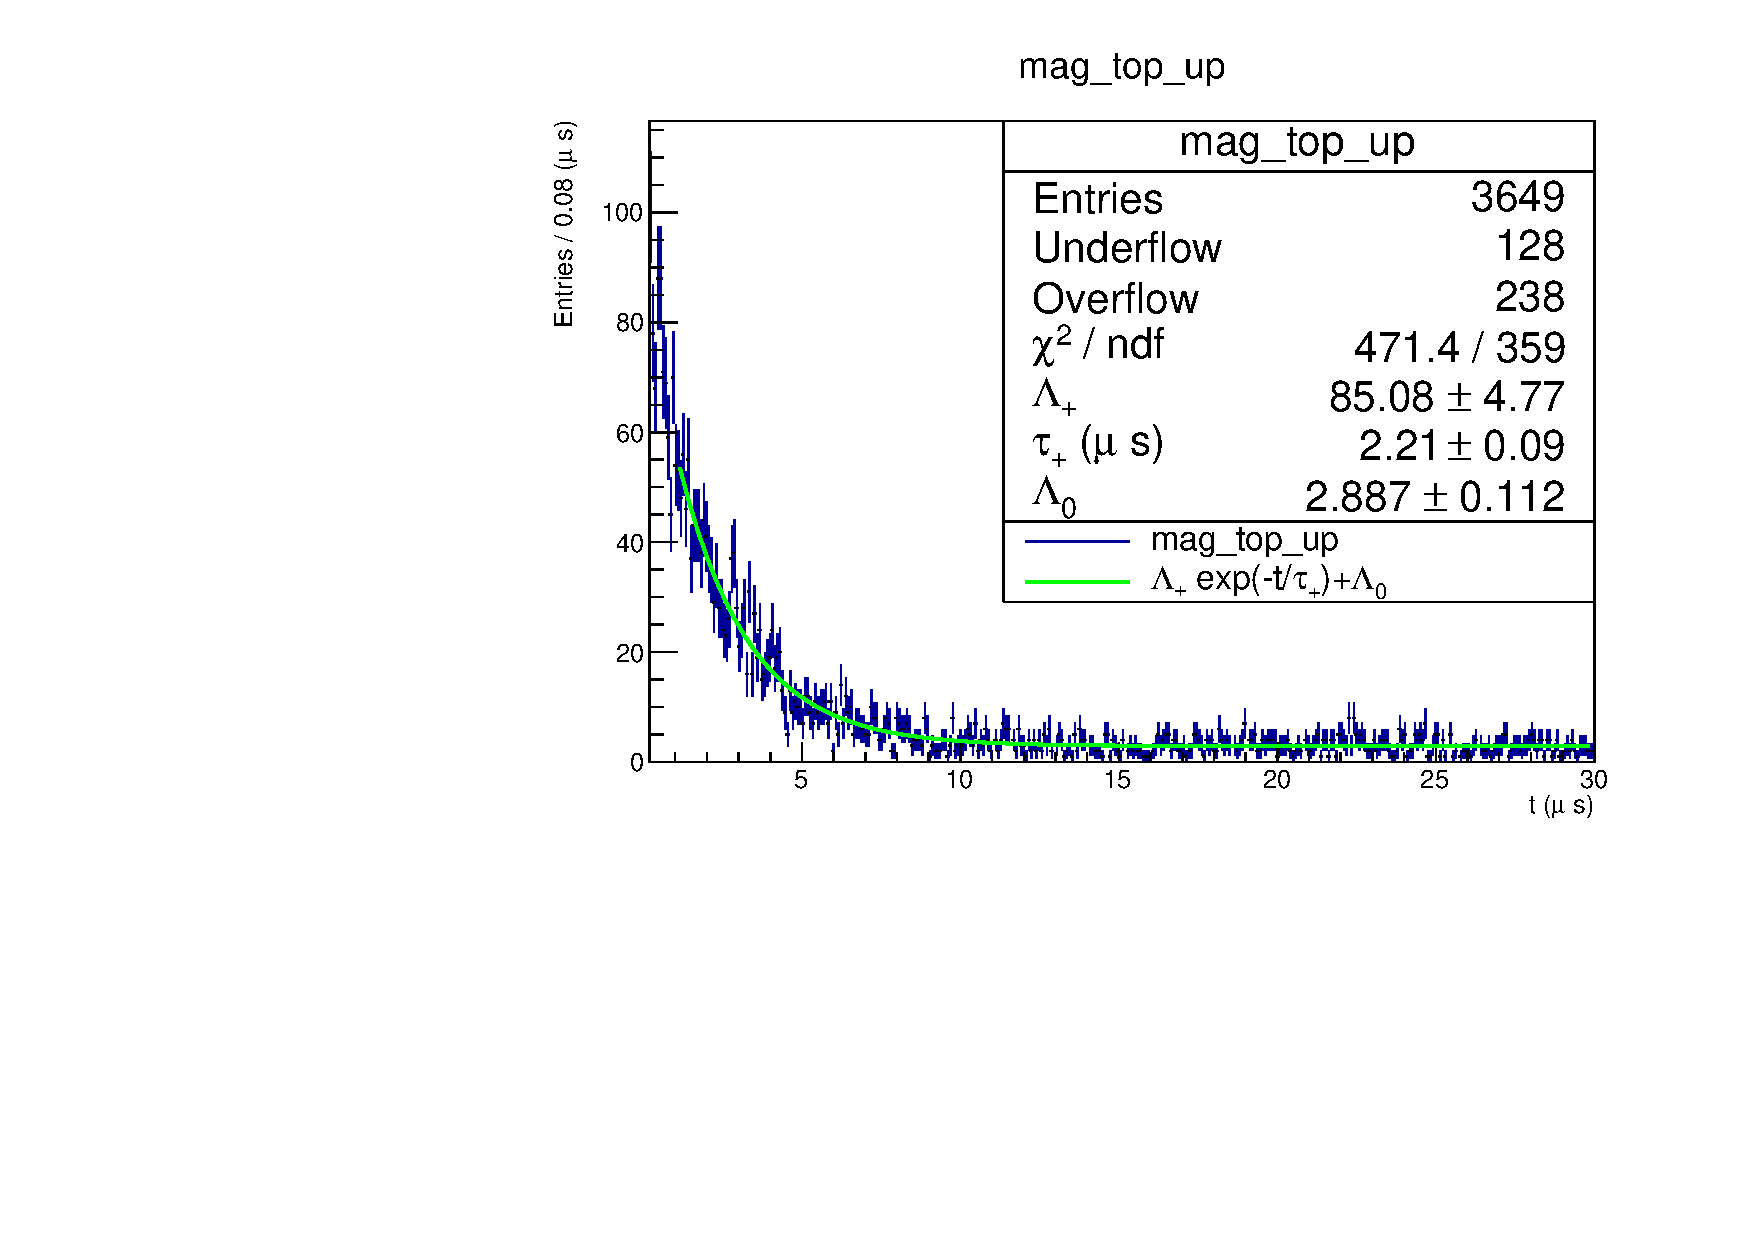
\includegraphics[scale=0.45]{Lab4/Mudecay/mag_top_up.pdf} 
\label{MAGTOPUP}
\end{figure}

\begin{figure}[h!]
\centering
\caption{Time distribution of Mag Fe TOP DOWN fitted in the range [1, 30] $\mu s$. [25-26-30/05/22]}
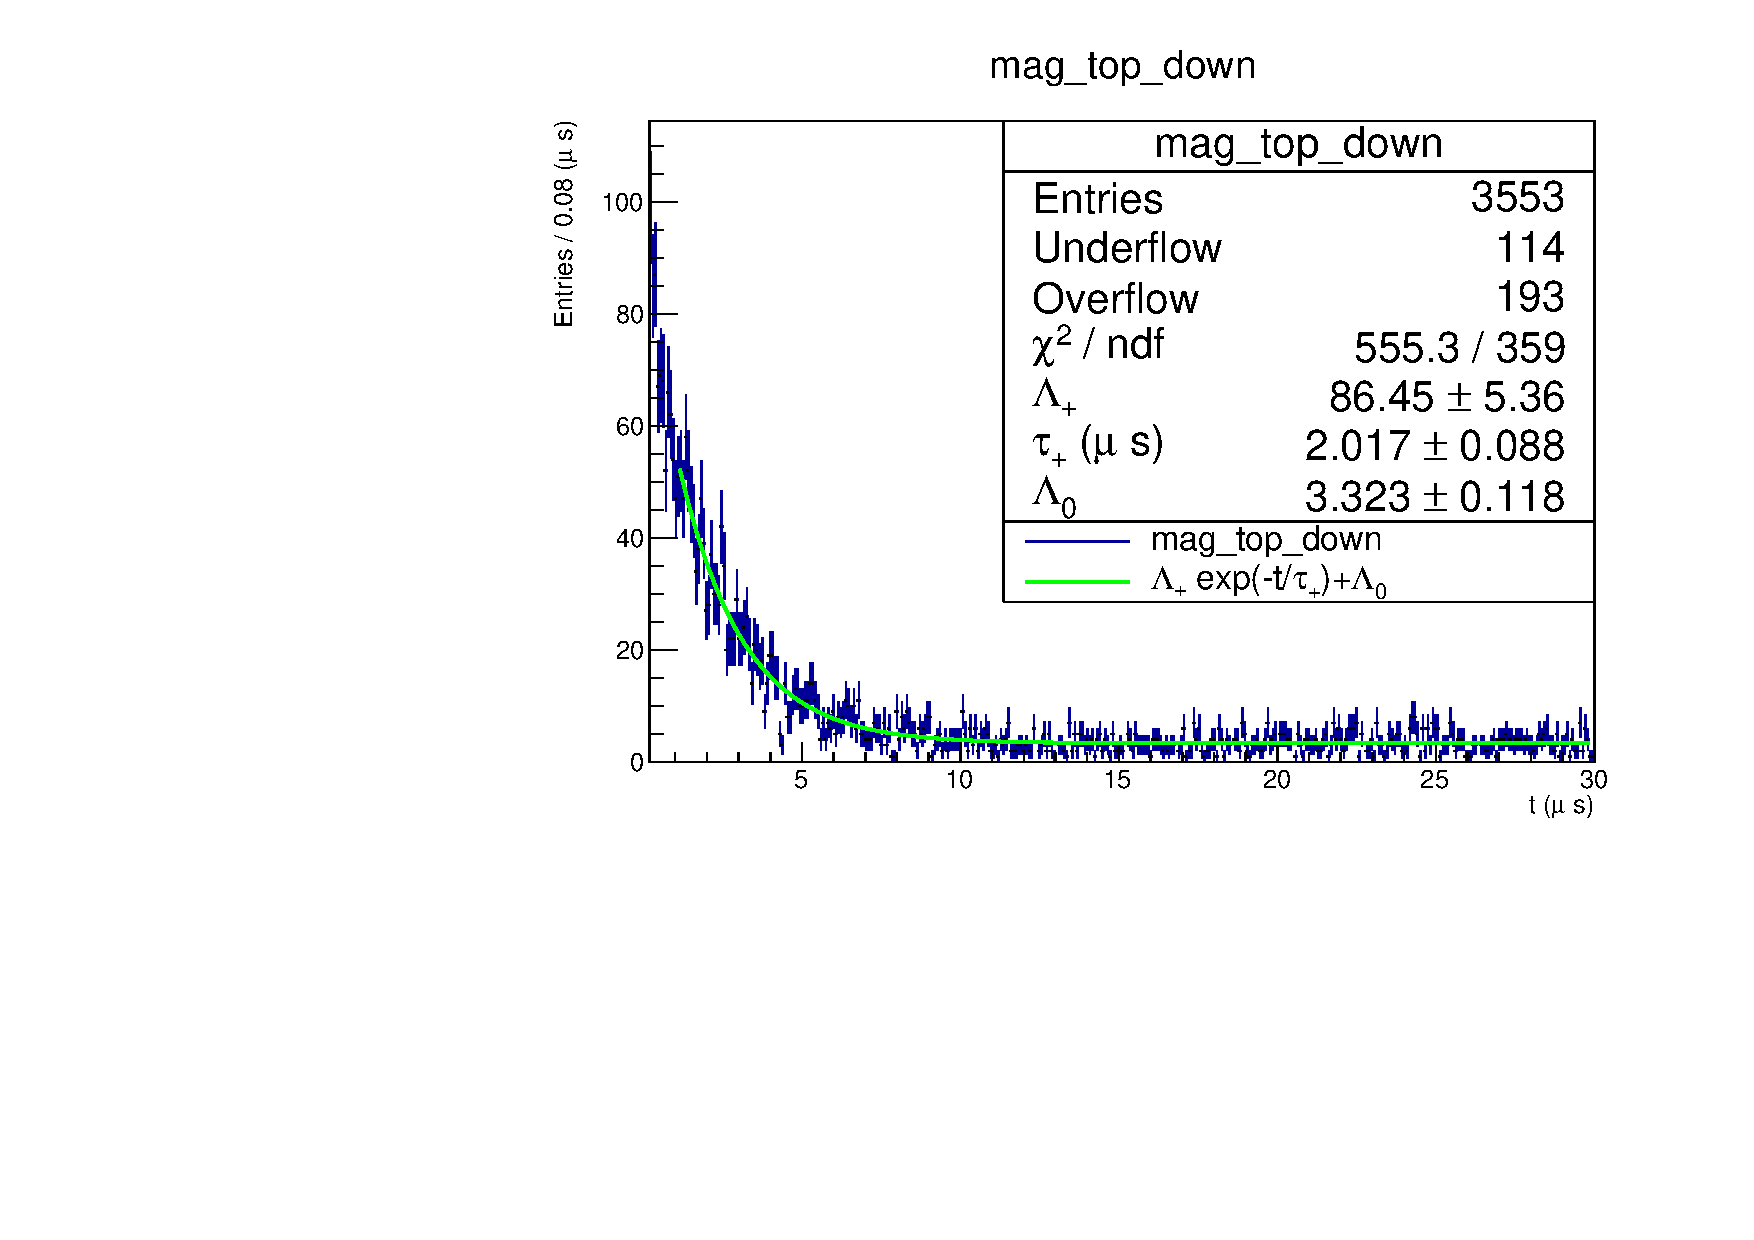
\includegraphics[scale=0.45]{Lab4/Mudecay/mag_top_down.pdf}
\label{MAGTOPDW}
\end{figure}

\begin{figure}[h!]
\centering
\caption{Time distribution of Mag Fe BOT UP fitted in the range [1, 30] $\mu s$. [18-19-24/05/22]}
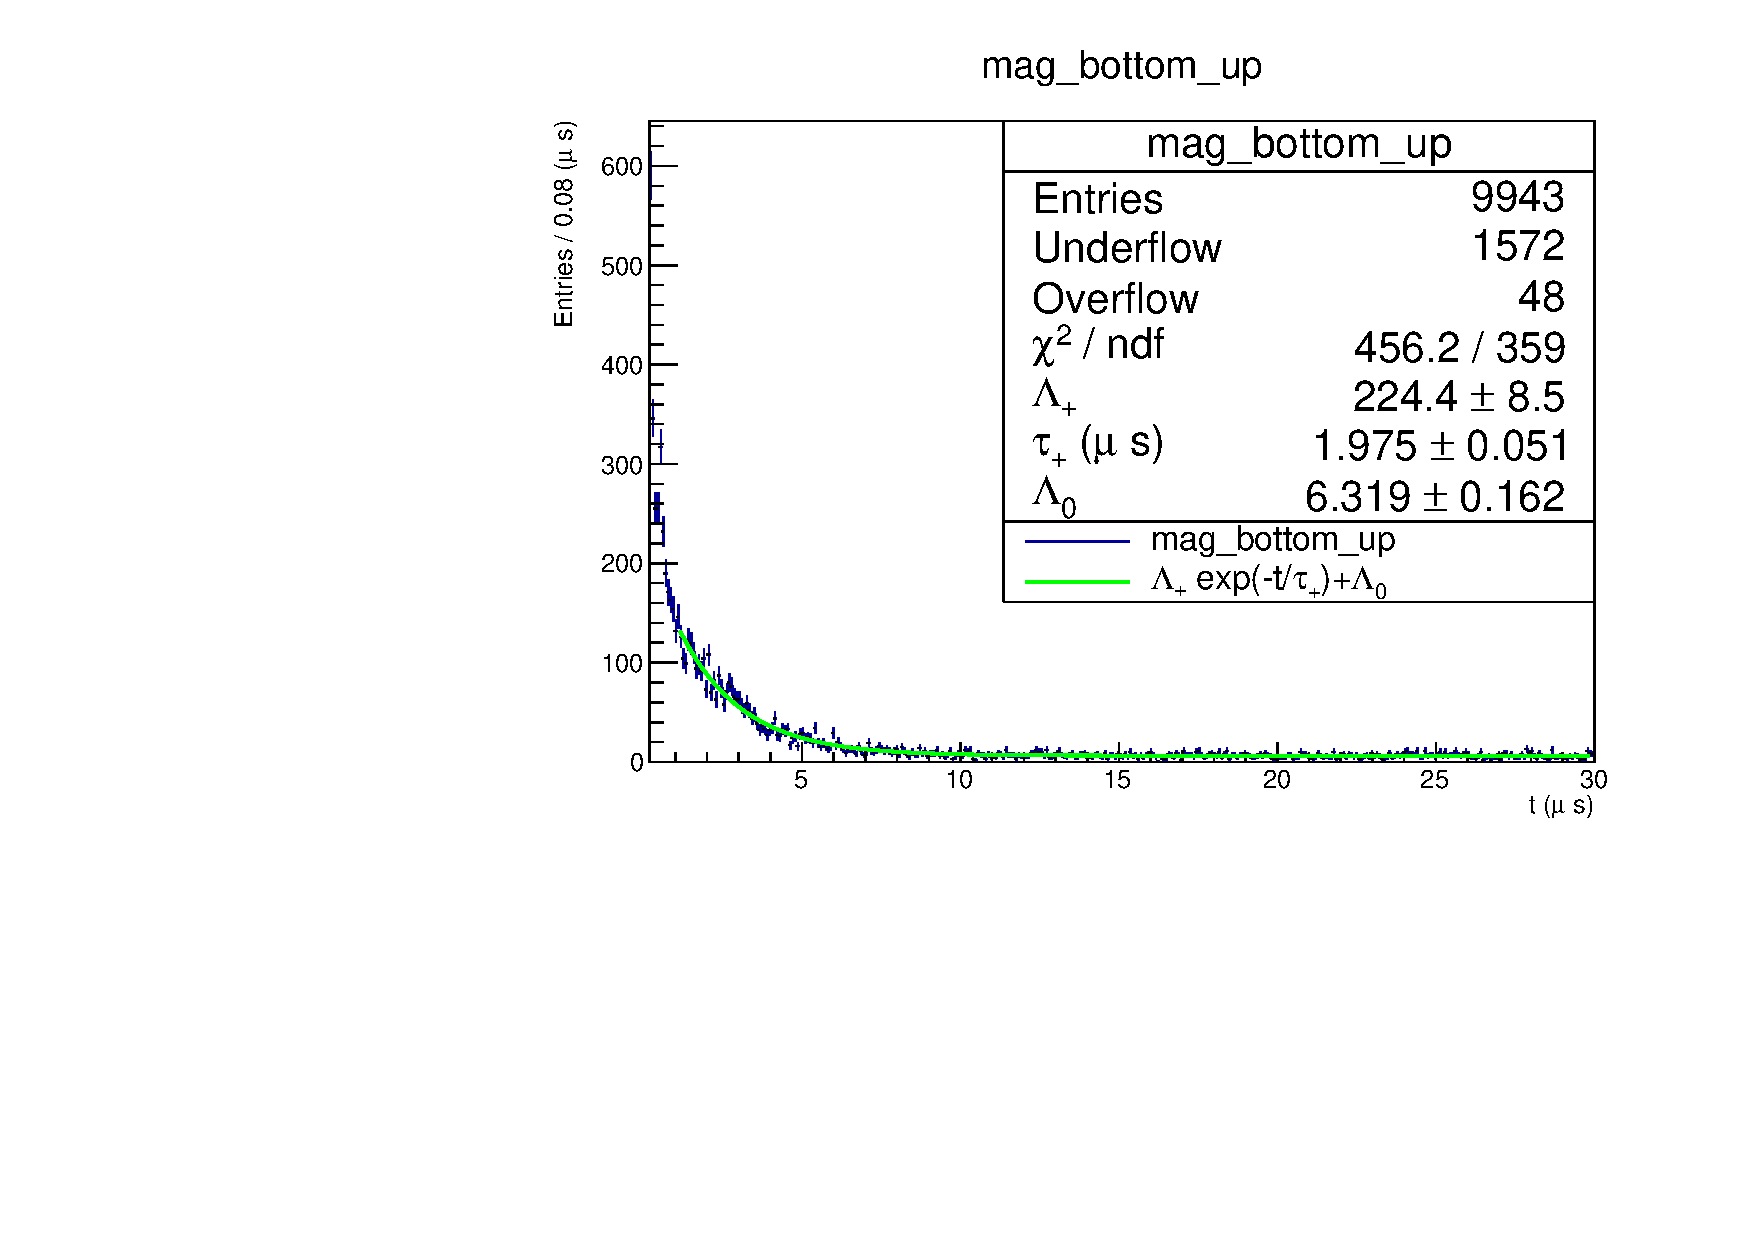
\includegraphics[scale=0.45]{Lab4/Mudecay/mag_bottom_up.pdf}
\label{MAGBOTUP}
\end{figure}

\begin{figure}[h!]
\centering
\caption{Time distribution of Mag Fe BOT DOWN fitted in the range [1, 30] $\mu s$. [18-19-24/05/22]}
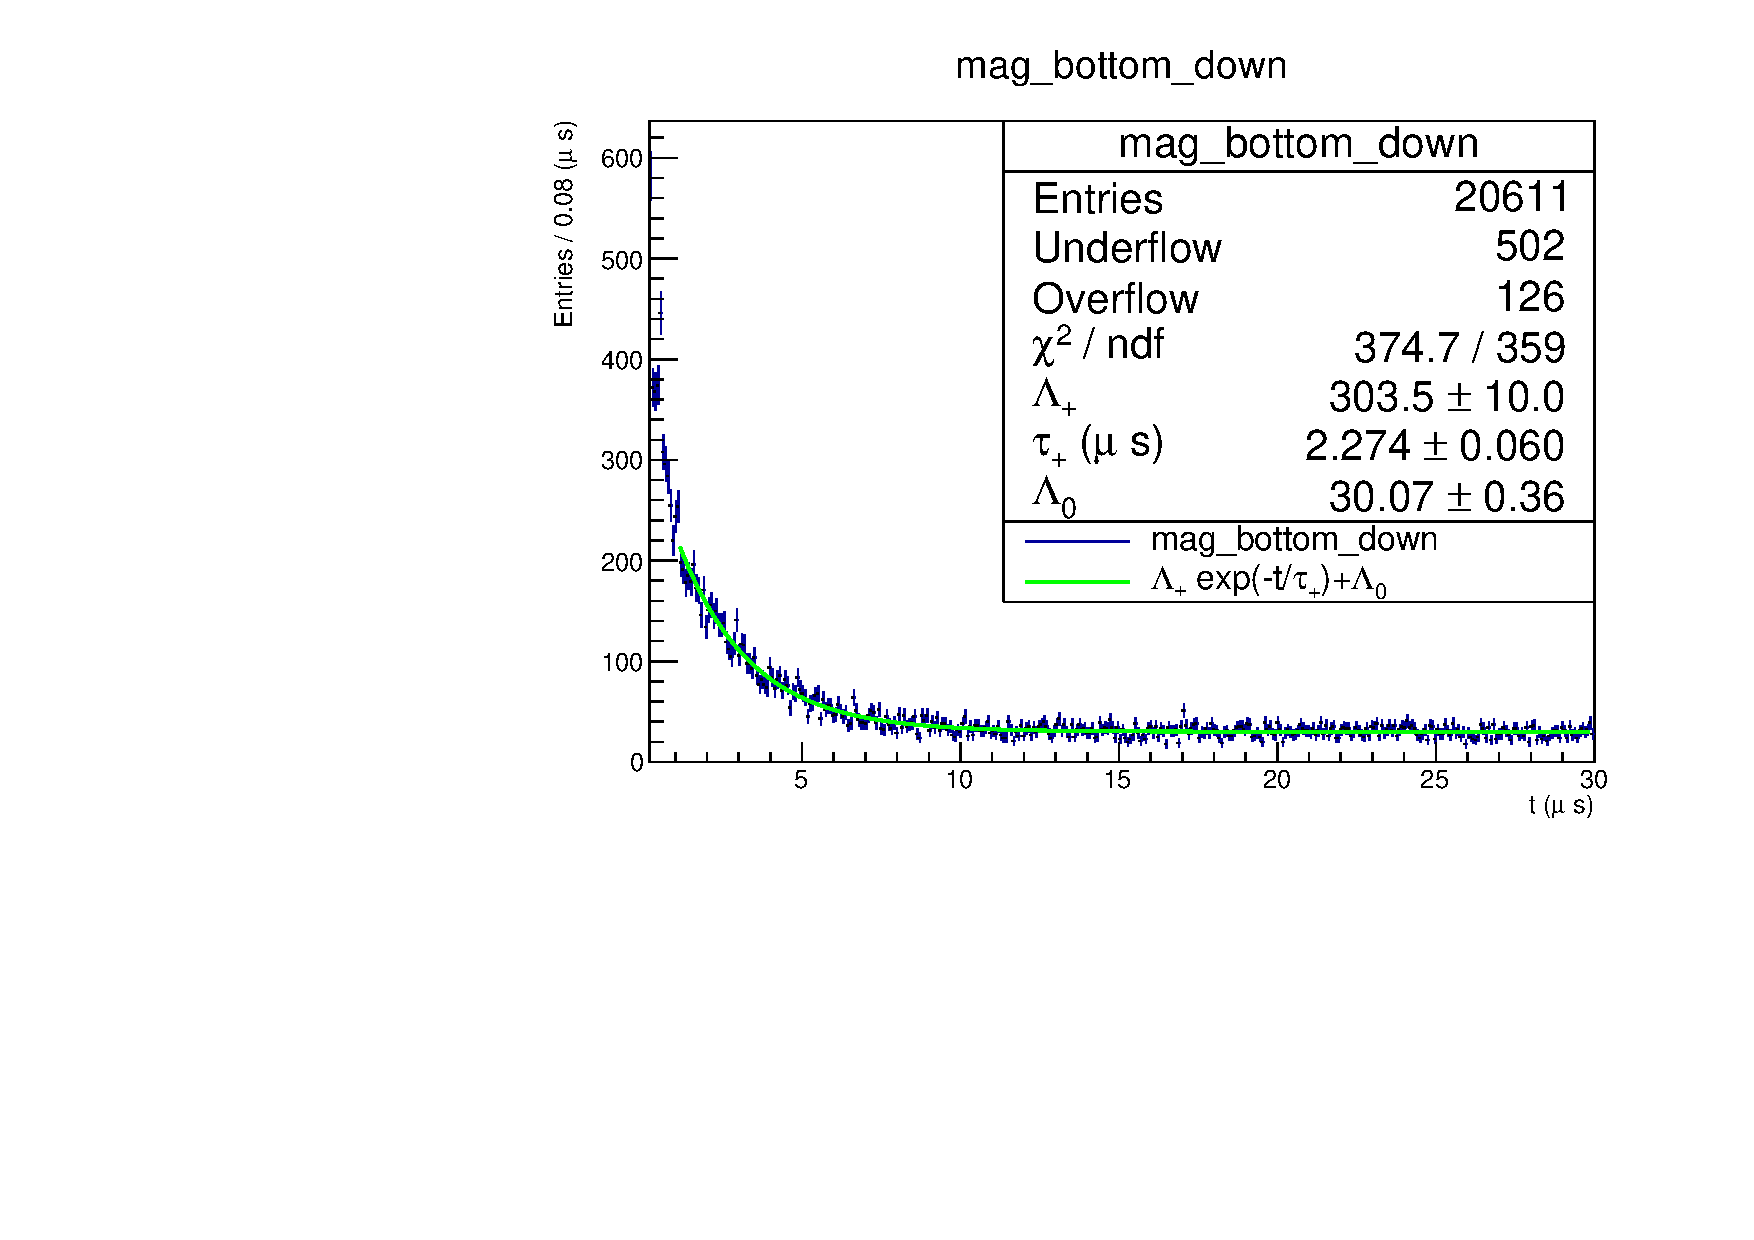
\includegraphics[scale=0.45]{Lab4/Mudecay/mag_bottom_down.pdf} 
\label{MAGBOTDW}
\end{figure}

Since the UP and DOWN of the TOP section are compatible with each other within just over one standard deviation and are independent (different scintillators), they are merged and fitted as shown in Figure \ref{MAGTOP}.

\begin{figure}[h!]
\centering
\caption{Time distribution of Mag Fe TOP TOT fitted in the range [1, 30] $\mu s$. [25-26-30/05/22]}
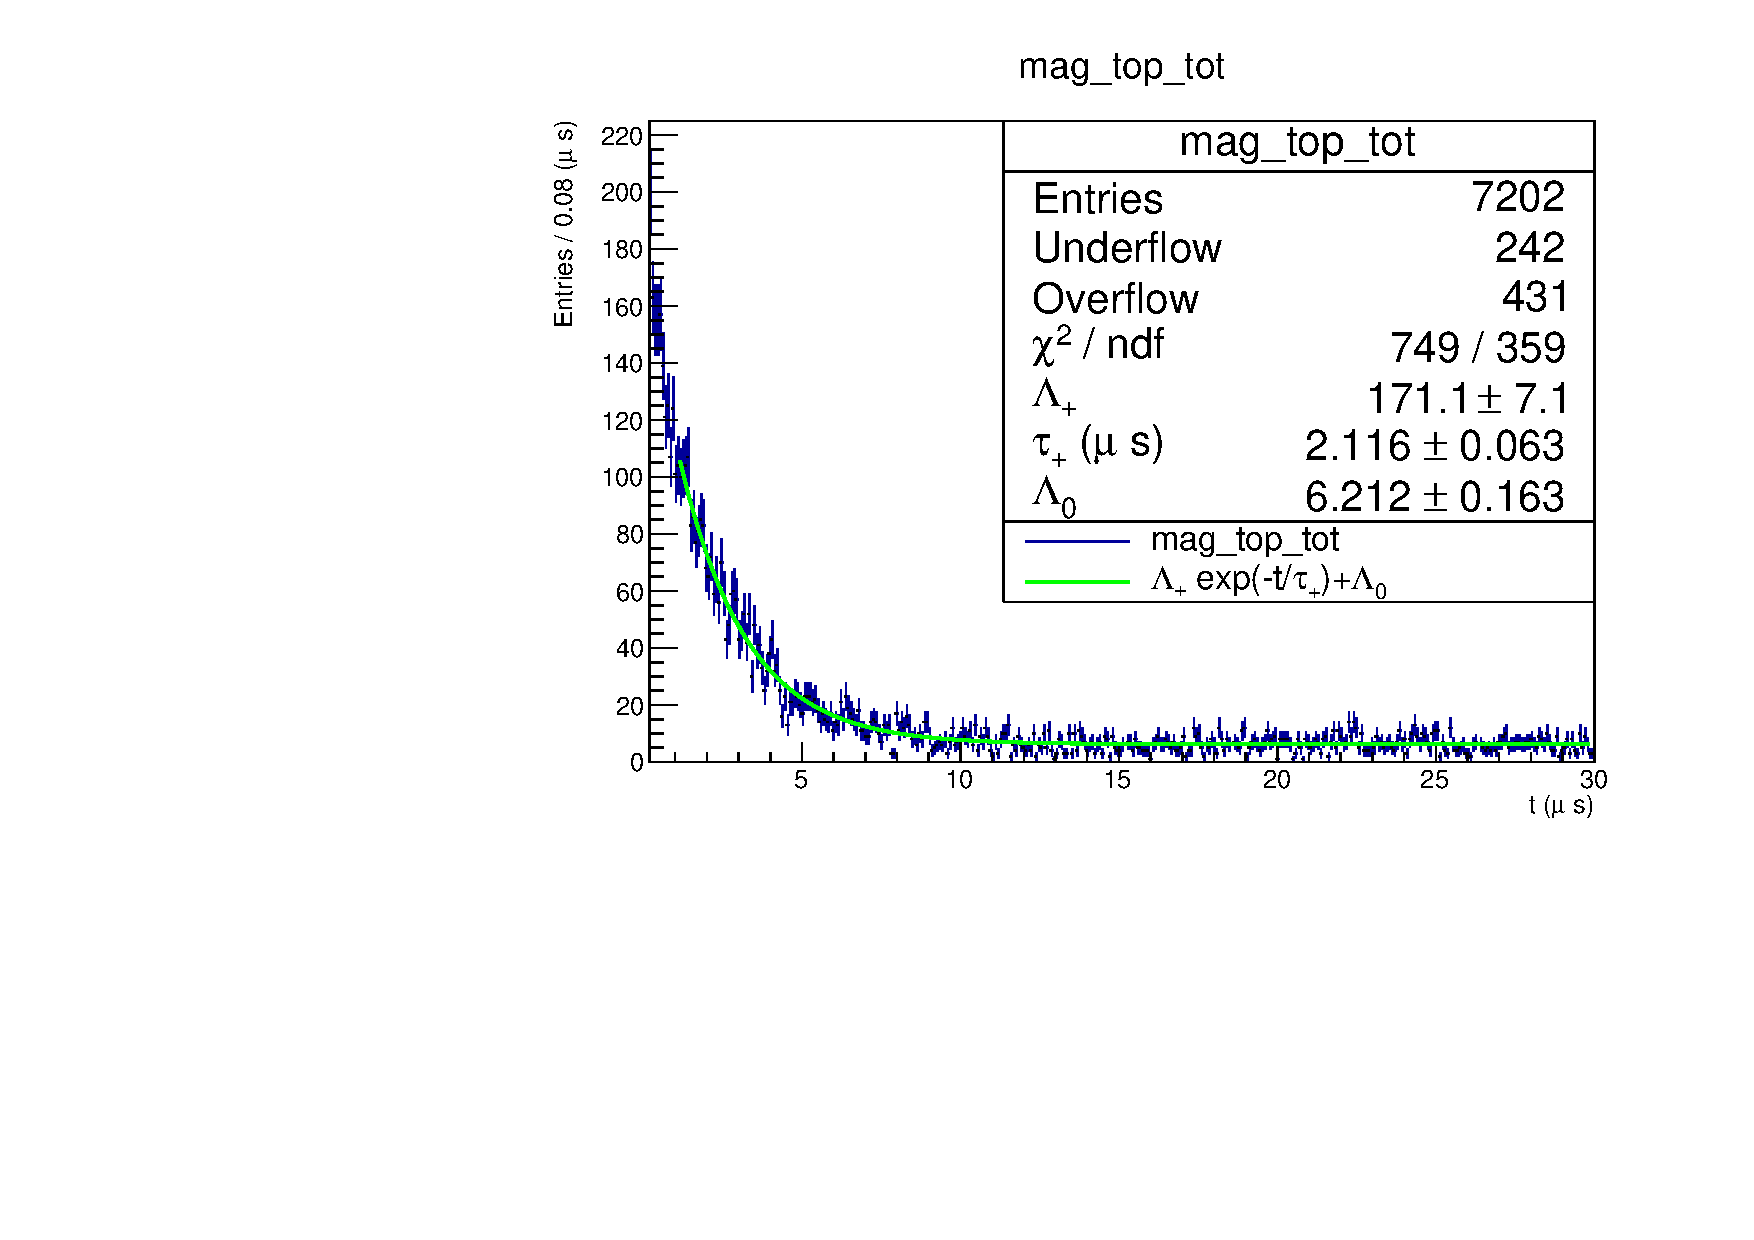
\includegraphics[scale=0.45]{Lab4/Mudecay/mag_top_tot.pdf} 
\label{MAGTOP}
\end{figure}

This fit yields  $\tau_+^{TOP}=2.12 \pm 0.06 \text{ (stat)} \pm 0.02 \text{ (syst) }$ which is compatible with the expected value within one standard deviation.

\\
[$\mu$s and $\tau_+^{BOT}=2.16 \pm 0.04 \text{ (stat)} \pm 0.03 \text{ (syst) }\mu$s. ( total $\tau_+=2.15 \pm 0.04 \text{ (stat)} \pm 0.02 \text{ (syst) }\mu$s.)]

\subsection{Combined measurement of $\tau_+$}
The various estimates for $\tau_+$, obtained by combining UP and DOWN when compatible with each other, are shown in Figure \ref{comb_tau_tot}. For these fits unfortunately the GOF parameter $\chi^2$ is quite high, on average $1.5\times$DOF.

\begin{figure*}[h!]
\centering
\caption{Various estimates of $\tau_+$. [10-11-12-17-18-19-25-26-27-30/05/22]}
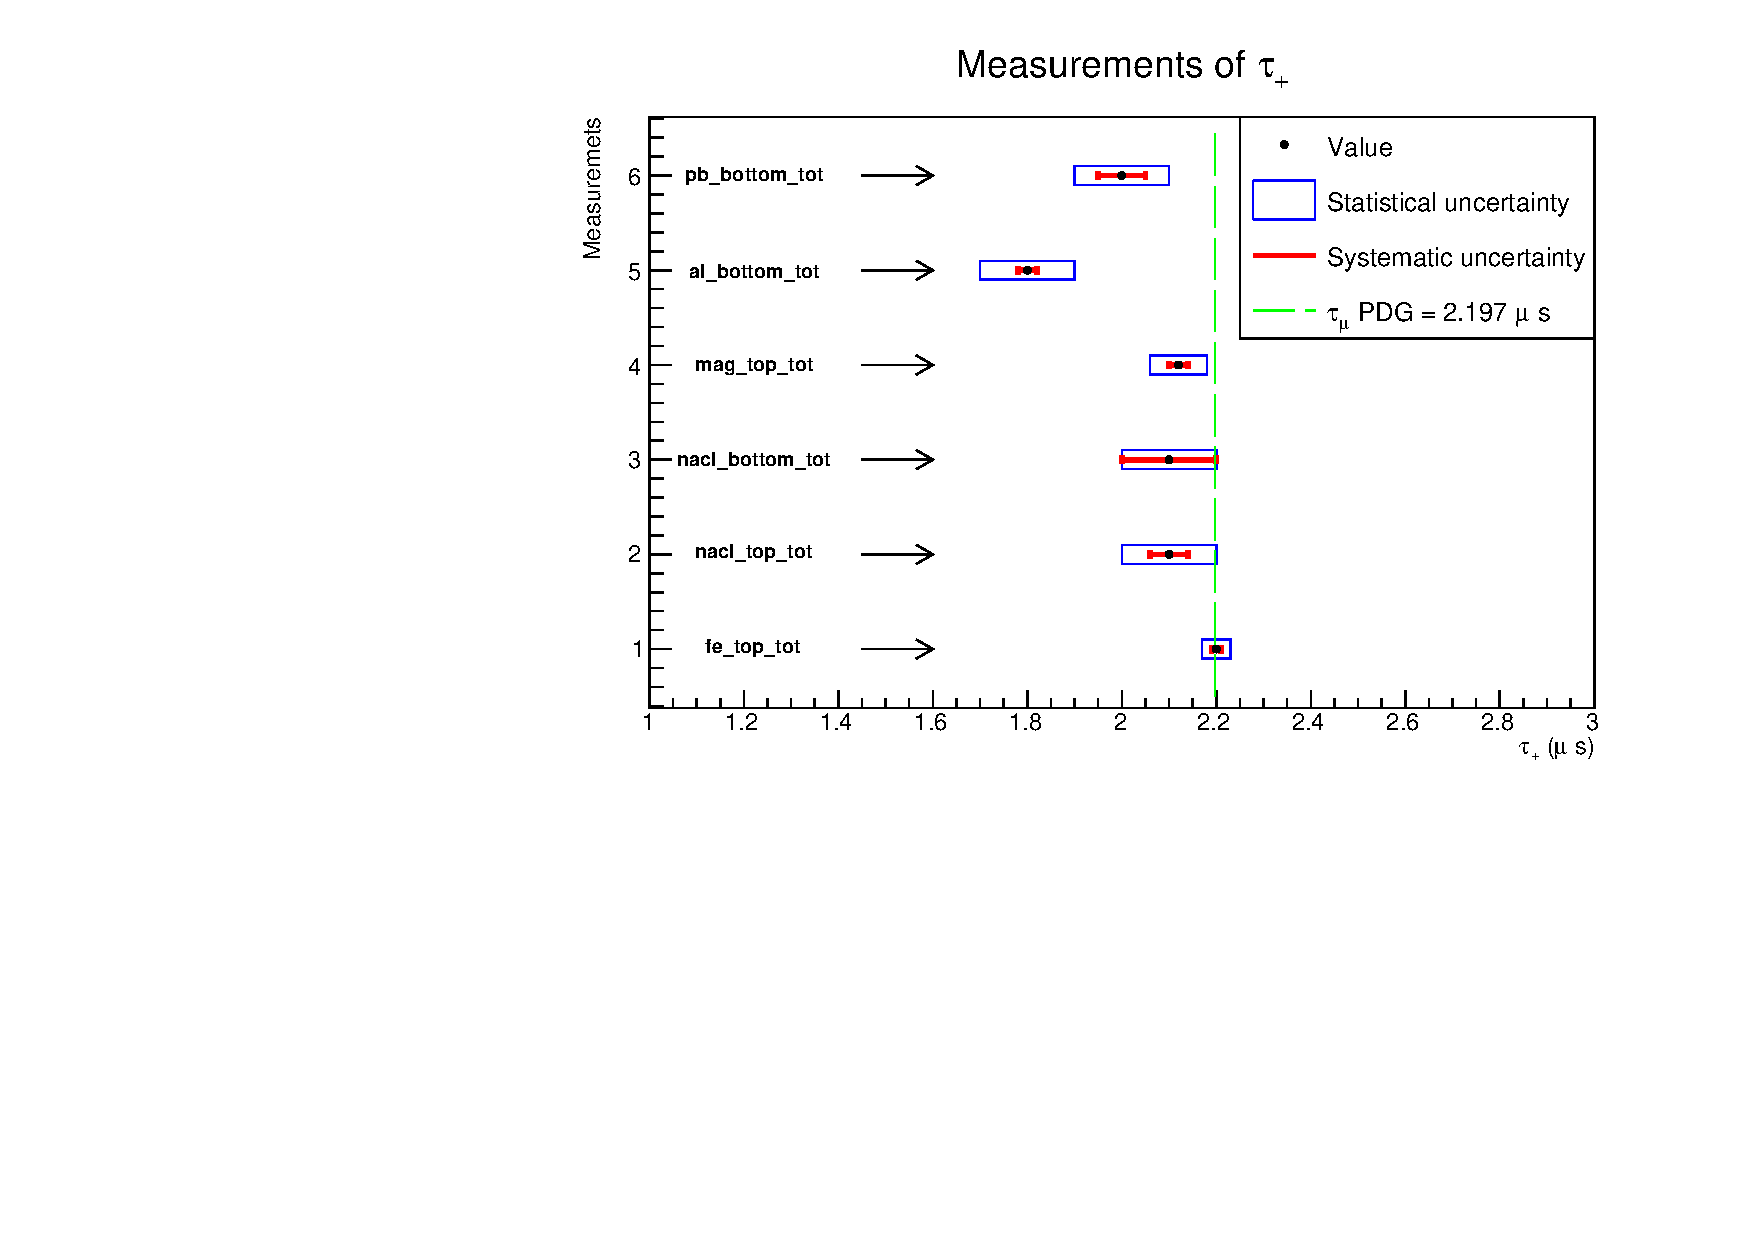
\includegraphics[scale=0.91]{Lab4/Mudecay/tau_long_tot.pdf} 
\label{comb_tau_tot}
\end{figure*}

Furthermore, in the assumption that the groups of PMT used as STOP (5$\cdot$6, 3$\cdot$4, 2) are independent, three of the measurements above, one for each group, were averaged using as weights the inverse of their variances. The measurements in question are:

\begin{itemize}
   \item $ \tau_+^{fe\_top\_up}& = 2.20 \pm 0.05 \text{ (stat)} \pm 0.03 \text{ (syst) }\mu s $
   \item $    \tau_+^{fe\_top\_down}& = 2.20 \pm 0.04 \text{ (stat)} \pm 0.02 \text{ (syst) }\mu s$
   \item $\tau_+^{nacl\_bottom\_down} = 2.2 \pm 0.2 \text{ (stat)} \pm 0.1 \text{ (syst) }\mu s$
\end{itemize}


and are reported in Figure \ref{tau_long_ave}.

\begin{figure*}[h!]
\centering
\caption{Combined estimates of $\tau_+$. [10-11-12-17-18-19-25-26-27-30/05/22]}
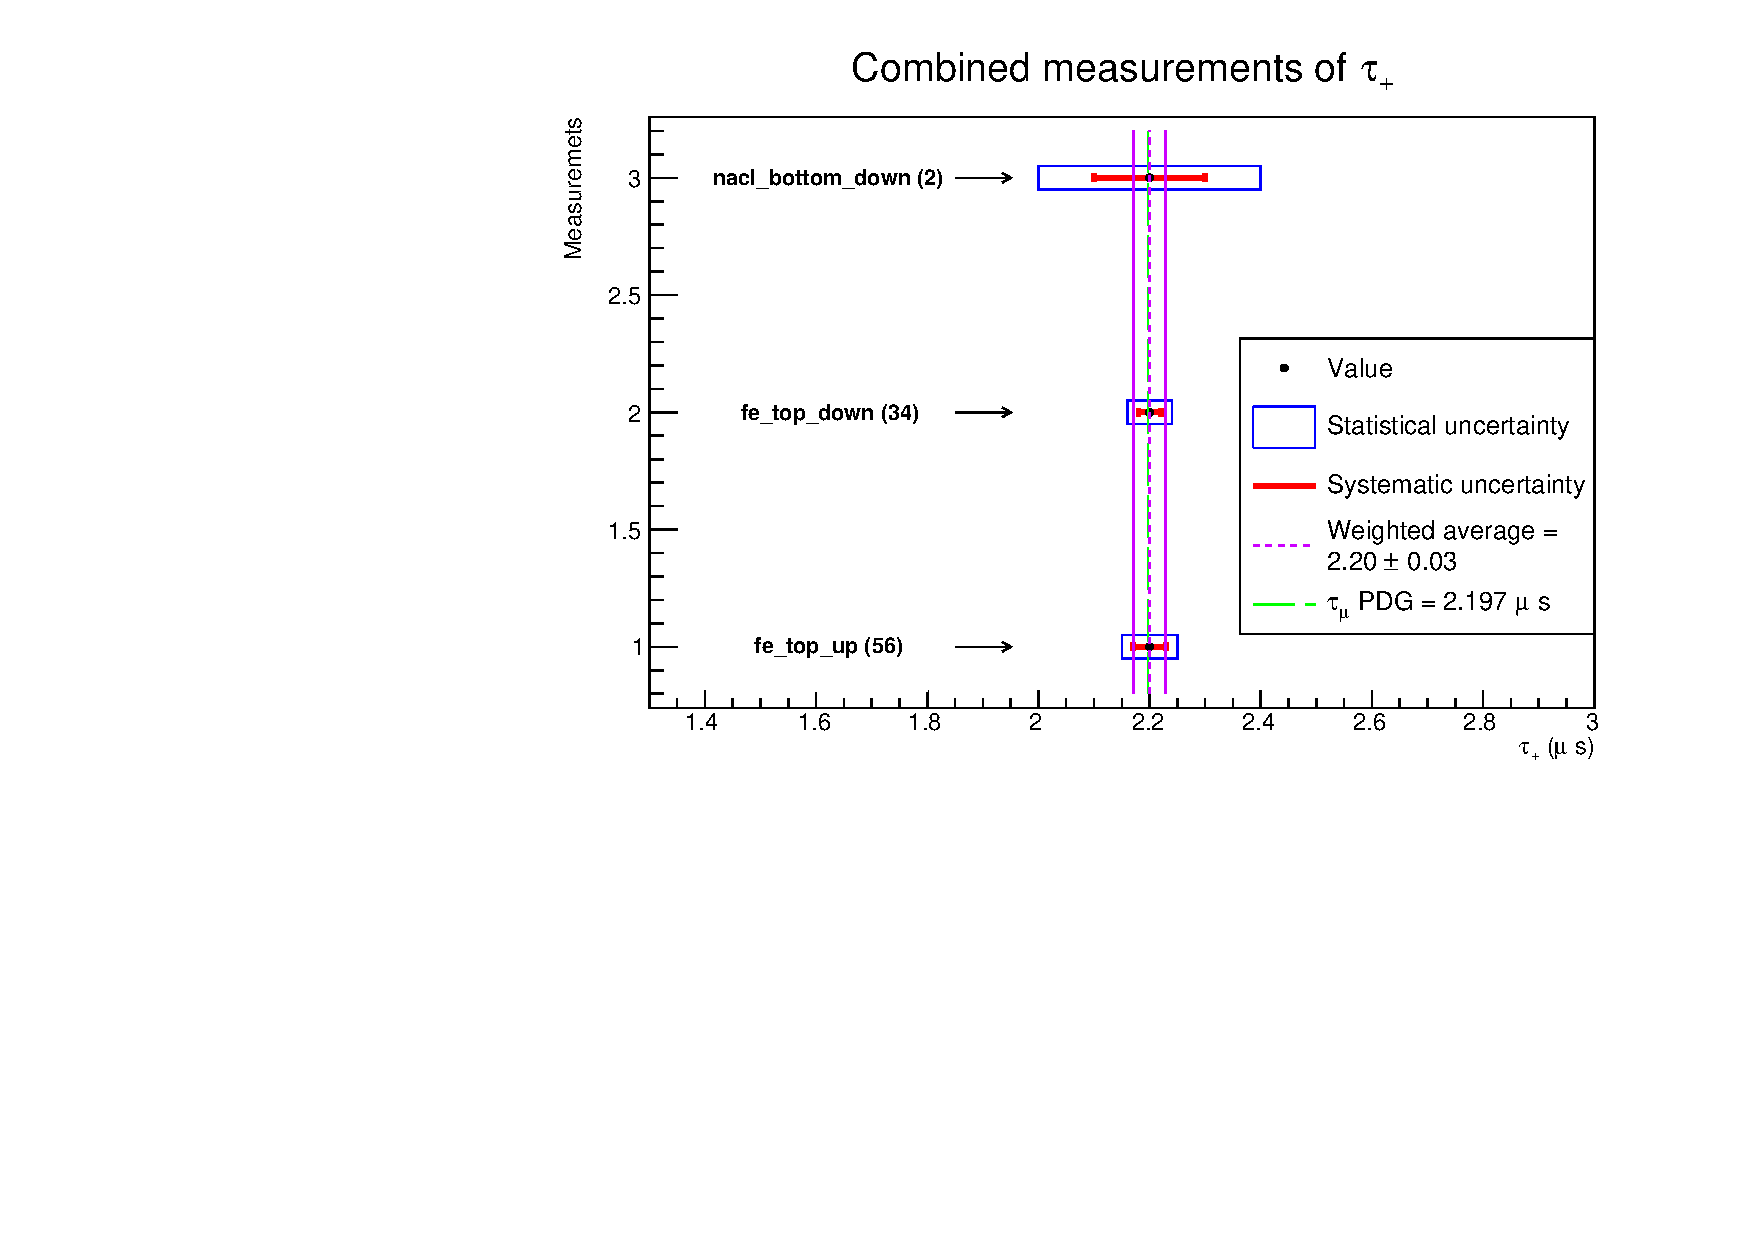
\includegraphics[scale=0.91]{Lab4/Mudecay/tau_long_ave.pdf} 
\label{tau_long_ave}
\end{figure*}

The final result yields $\tau_+ = 2.20 \pm 0.03 \text{ (stat)} \pm 0.11 \text{ (syst) }\mu s$, where as systematical uncertainty was taken the sum of the squares of the systematical uncertainties of the measurements in question. 

\section{Pedestal and afterpulse peak}

In the $t$ distributions observed there is a pedestal of events in the region $\lesssim$150 ns. One specific problem with the UP samples was that when STOPUP is activated there is a certain chance that START is activated too since it is a particular subcase of STOPUP. Therefore if one subtracts to the STOPUP timestamp the nearest previous START timestamp one often finds a null difference (Figure \ref{pedestalnocorrection}). This can be fixed by, in these cases, taking as START signal the \textit{second} most recent one.

\begin{figure}[h!]
\centering
\caption{Time distribution of Fe TOP UP in the range [-0.1, 1] $\mu s$ without the pedestal correction. [10/05/22]}

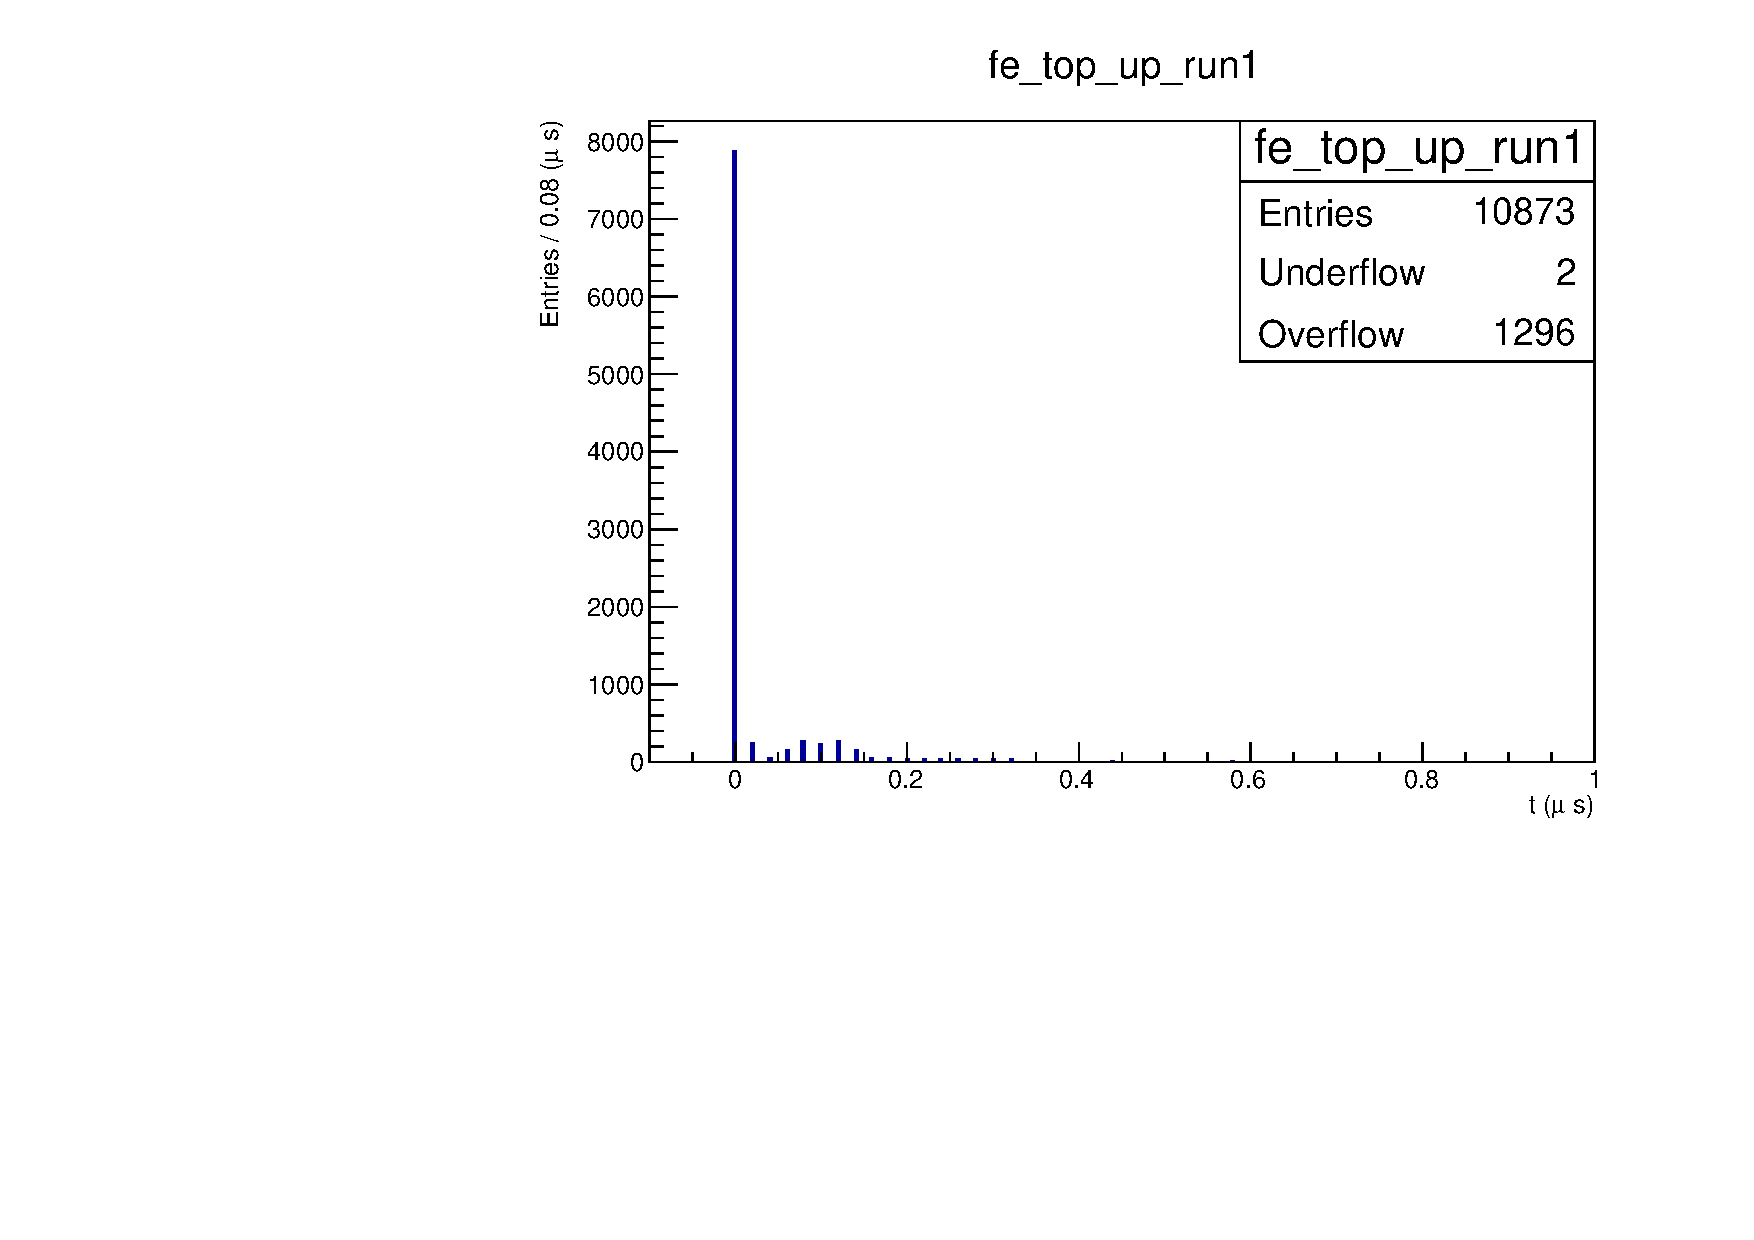
\includegraphics[scale=0.45]{Lab4/Mudecay/pedestal.pdf} 
\label{pedestalnocorrection}
\end{figure}

Even with this correction and delaying the GATE by $\sim$2 times the length of the START signal itself, the pedestal remains present, as can be seen in Figure \ref{pedestalcorrection}. The delay of the GATE was later pushed to 108 ns for the last runs, since the region under 150 ns was not made use of anyway, due to the pedestal. 

\begin{figure}[h!]
\centering
\caption{Time distribution of Fe TOP UP in the range [-0.1, 1] $\mu s$ with the pedestal correction. [10/05/22]}
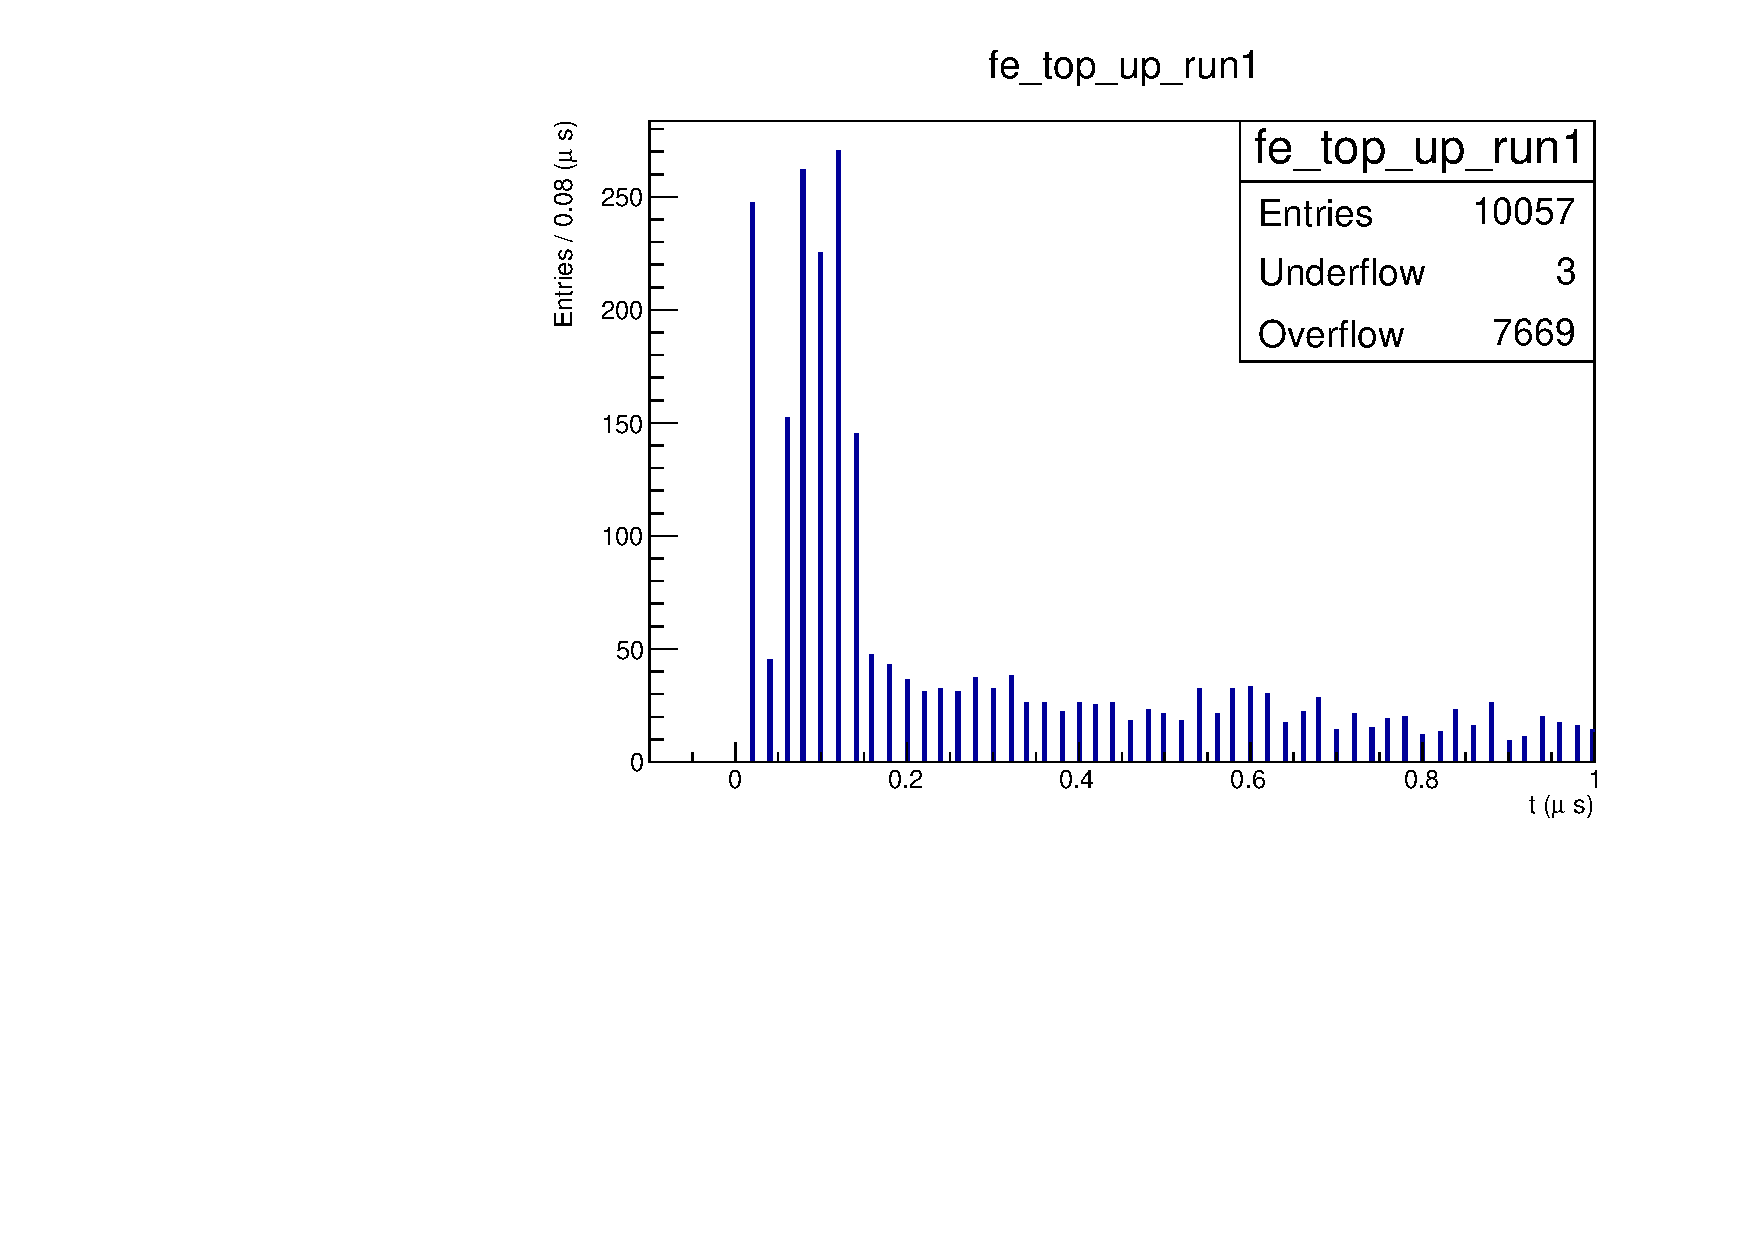
\includegraphics[scale=0.45]{Lab4/Mudecay/no_pedestal.pdf} 
\label{pedestalcorrection}
\end{figure}
\\
\\
An interesting phenomenon is that is every type of sample, and more intensely in BOT DOWN samples, there is a peak of events around 550-600 ns. This cannot be due to a contamination of materials in which muons decay, since it is not an exponential. Nor can it be due to false starts in the circuitry, since the durations of the signals used in the NIM circuits is of the order of a few tens of ns.
\\
On the other hand, it could be the effect of afterpulses in the scintillators. This would explain why the signal appears at a specific time in all samples and why it is overwhelmingly more relevant precisely in the DOWN BOT samples, where the STOP is only given by \textit{one} PMT. Calling $p$ the probability of an afterpulse being detected, in samples in which the STOP is given by two scintillators the relative afterpulse peak should be suppressed by a factor $\sim p$. To check this, a run was made with START conditions $6\cdot 5\cdot 4 \cdot 3$ and $4\cdot 3\cdot 2$, so as to observe the distribution of STOPs that should \textit{not} be correlated with START. The results are plotted in Figure \ref{apbotdw}. Aside from the usual pedestal and approximately flat noise, there are two evident peaks: one at $\sim$ 250 ns and one just under 600 ns. These values are in line with afterpulse delays found in a variety of PMTs \cite{afterpulse2}, further suggesting that these peaks are afterpulses.
\\
\\
An interesting thing to note here is that DOWN BOT has a much (relatively) bigger peak at 600 ns respect to DOWN UP (Figure \ref{apbotup}). Calculating the probability of an event in said peak for DOWN BOT and for e.g. UP BOT , one finds, using a binomial approximation,

\bigbreak



\begin{equation*} 
p_{UP}  =63/926=6.8 \pm 0.8\% 
\end{equation*}

\begin{equation*} 
p_{DW}  =1843/9712=19.0 \pm 0.4\%  \rightarrow \sqrt{p_{DW}}=4.4 \pm 0.1
\end{equation*}


Even if not compatible, $p_{UP}$ and $\sqrt{p_{DW}}$ are very similar: $6.8\pm 0.8$ \% and $(19\%)^2 =$ 4.4 \%, within 50\% of each other. This suggests that the afterpulse interpretation is correct.
\\


\begin{figure}[h!]
\centering
\caption{Time distribution of the afterpulse BOT DOWN. [27/05/22]}
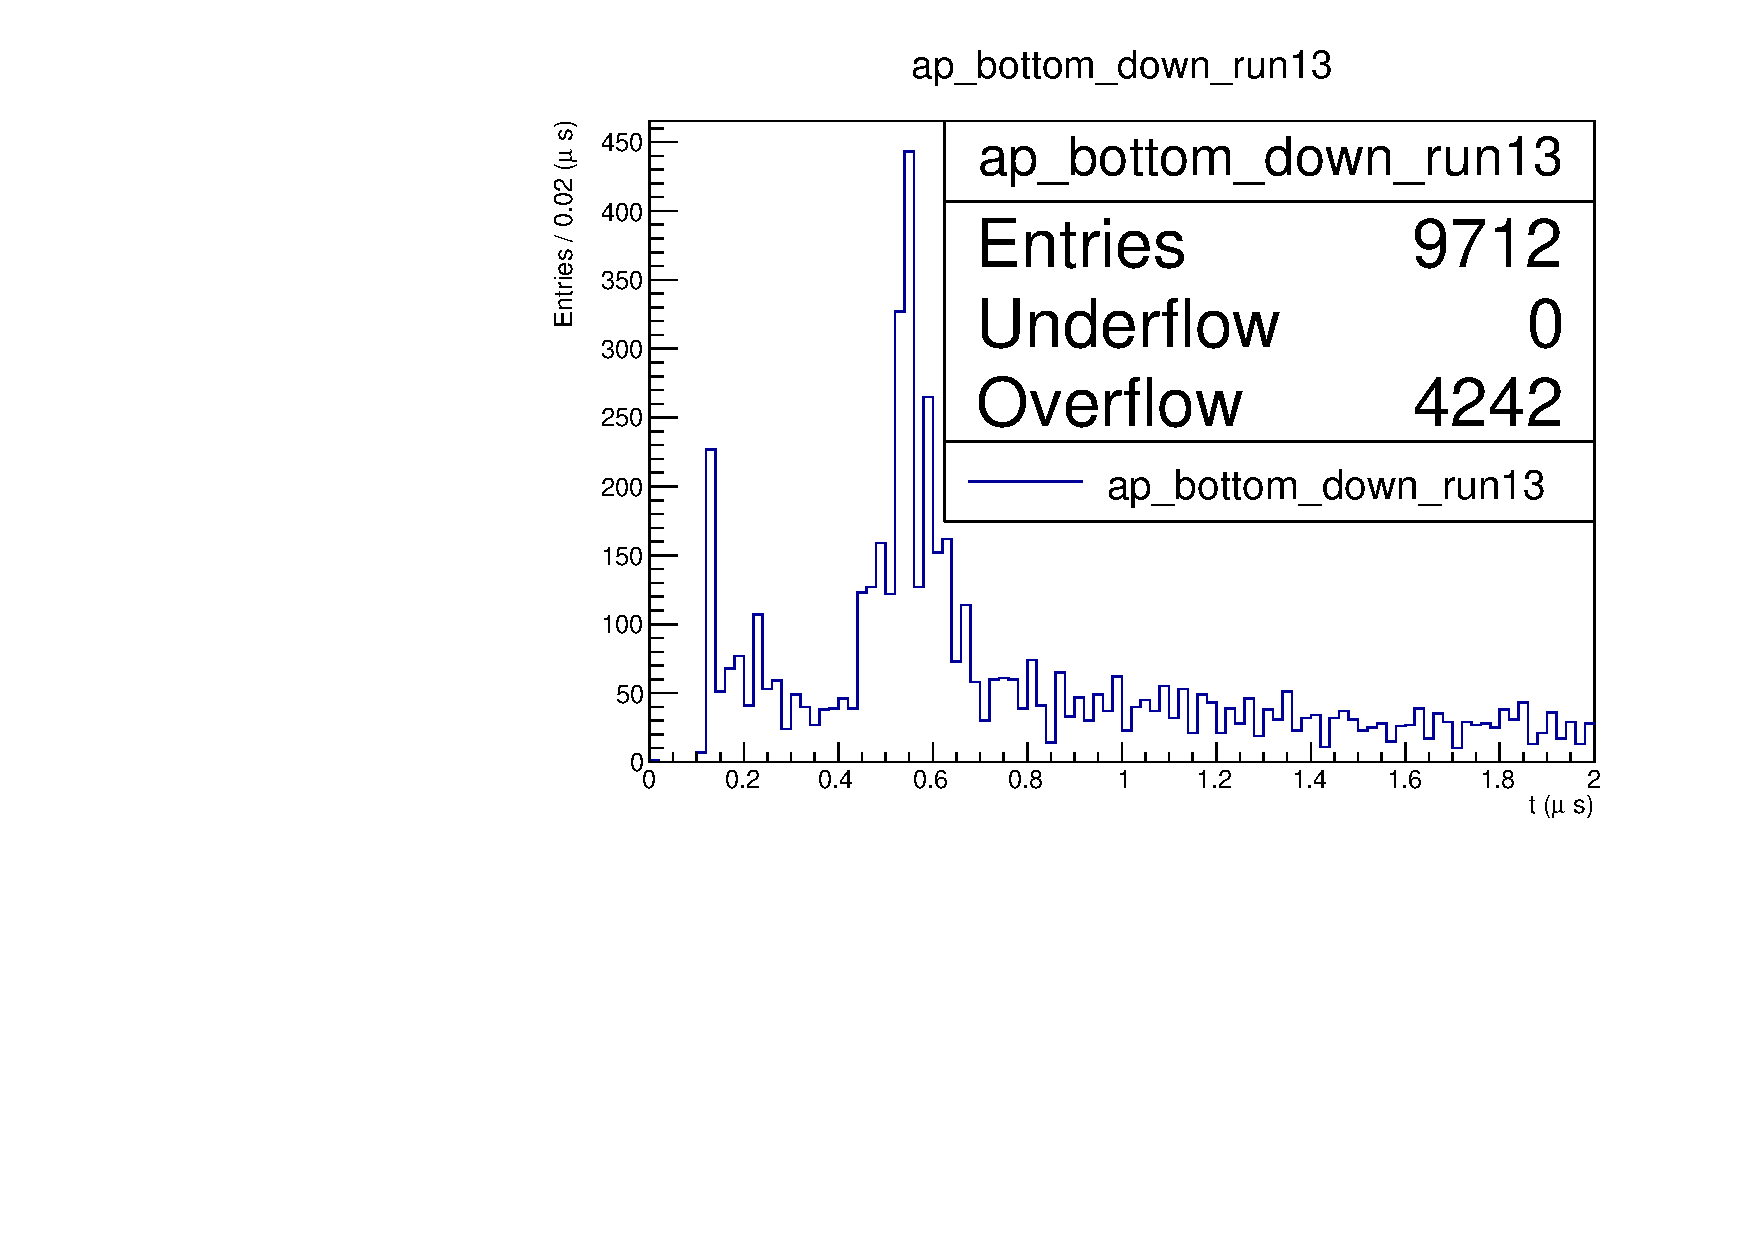
\includegraphics[scale=0.45]{Lab4/Mudecay/ap_bottom_down_run13.pdf} 
\label{apbotdw}
\end{figure}

\begin{figure}[h!]
\centering
\caption{Time distribution of the afterpulse BOT UP. [27/05/22]}
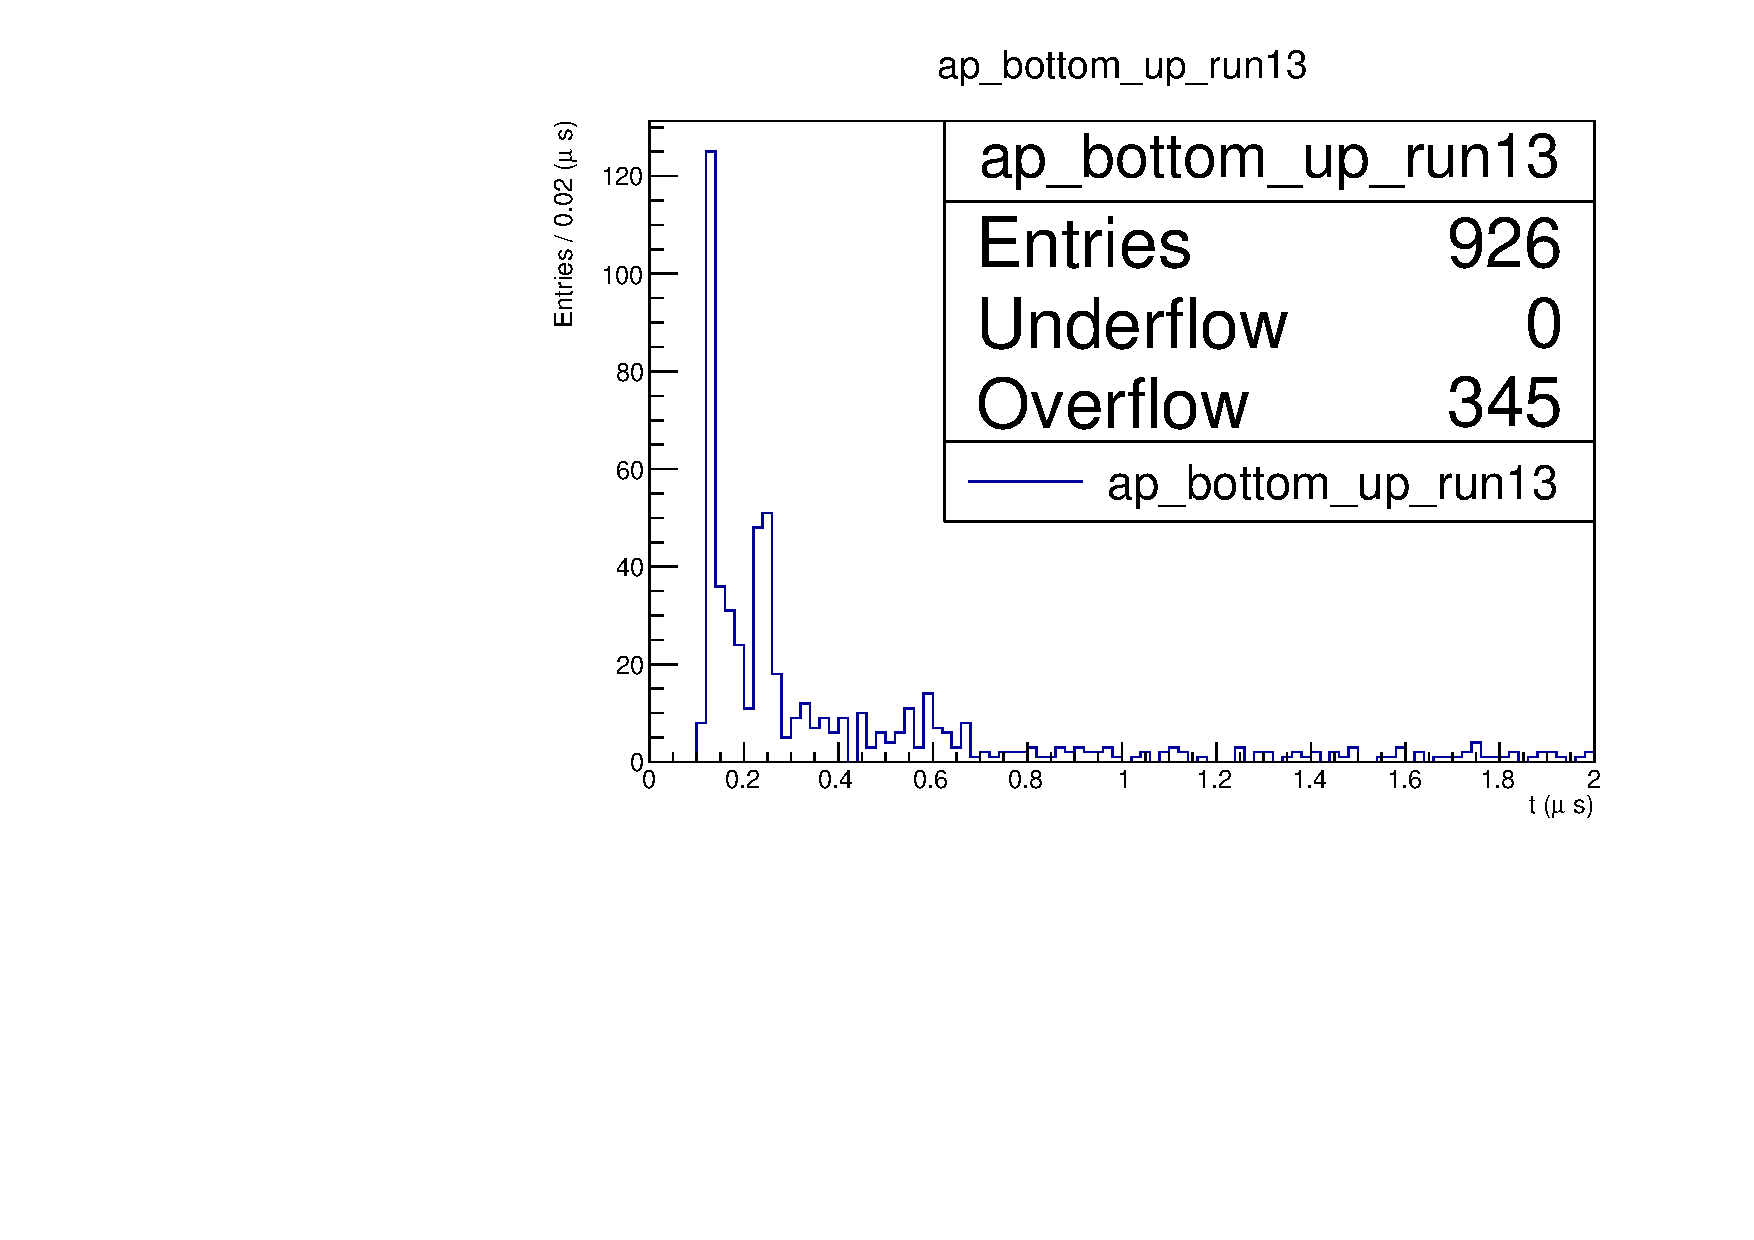
\includegraphics[scale=0.45]{Lab4/Mudecay/ap_bottom_up_run13.pdf} 
\label{apbotup}
\end{figure}

\section{Measurement of $\tau_-$}

While the method described in the past section is ideal to measure $\tau_+$, the same cannot be done with $\tau_-$. Hence a double exponential fit is mandatory.
\begin{equation}
    \label{expo_tot}
    p(t)=\Lambda_- e^{-t/\tau_-}+ \Lambda_+e^{-t/\tau_+}+\Lambda_0
\end{equation}


%As expected from such fitting model, it can be easily shown (Figure \ref{doubleexpotrouble}) that the fit of the same data can be made to converge to wildly different parameter values depending on the starting point given to the fitting algorithm.



Since, as already mentioned, double exponentials are notoriously hard to fit correctly, another approach was chosen. The fit is made up of two sub-fits:


The first is exclusively at high $t$, just like was done with $\tau_+$. From this fit one obtains $\Lambda_+$, $\tau_+$ and $\Lambda_0$ using a \textit{single} exponential model.

The second fit is done at lower $t$ with a double exponential model but with $\Lambda_+$, $\tau_+$ and $\Lambda_0$ fixed to their fitted values on the previous step.


\subsection{$\tau_-$ in Fe}
A similar procedure to the one for $\tau_+$ was followed, fitting separately the UP and DOWN data when using Fe (Figure \ref{FEUP-} \ref{FEDW-}).

\begin{figure}[h!]
\centering
\caption{Time distribution of Fe TOP UP fitted in the range [0.185, 30] $\mu s$. [10-11-12-17-19-26/05/22]}
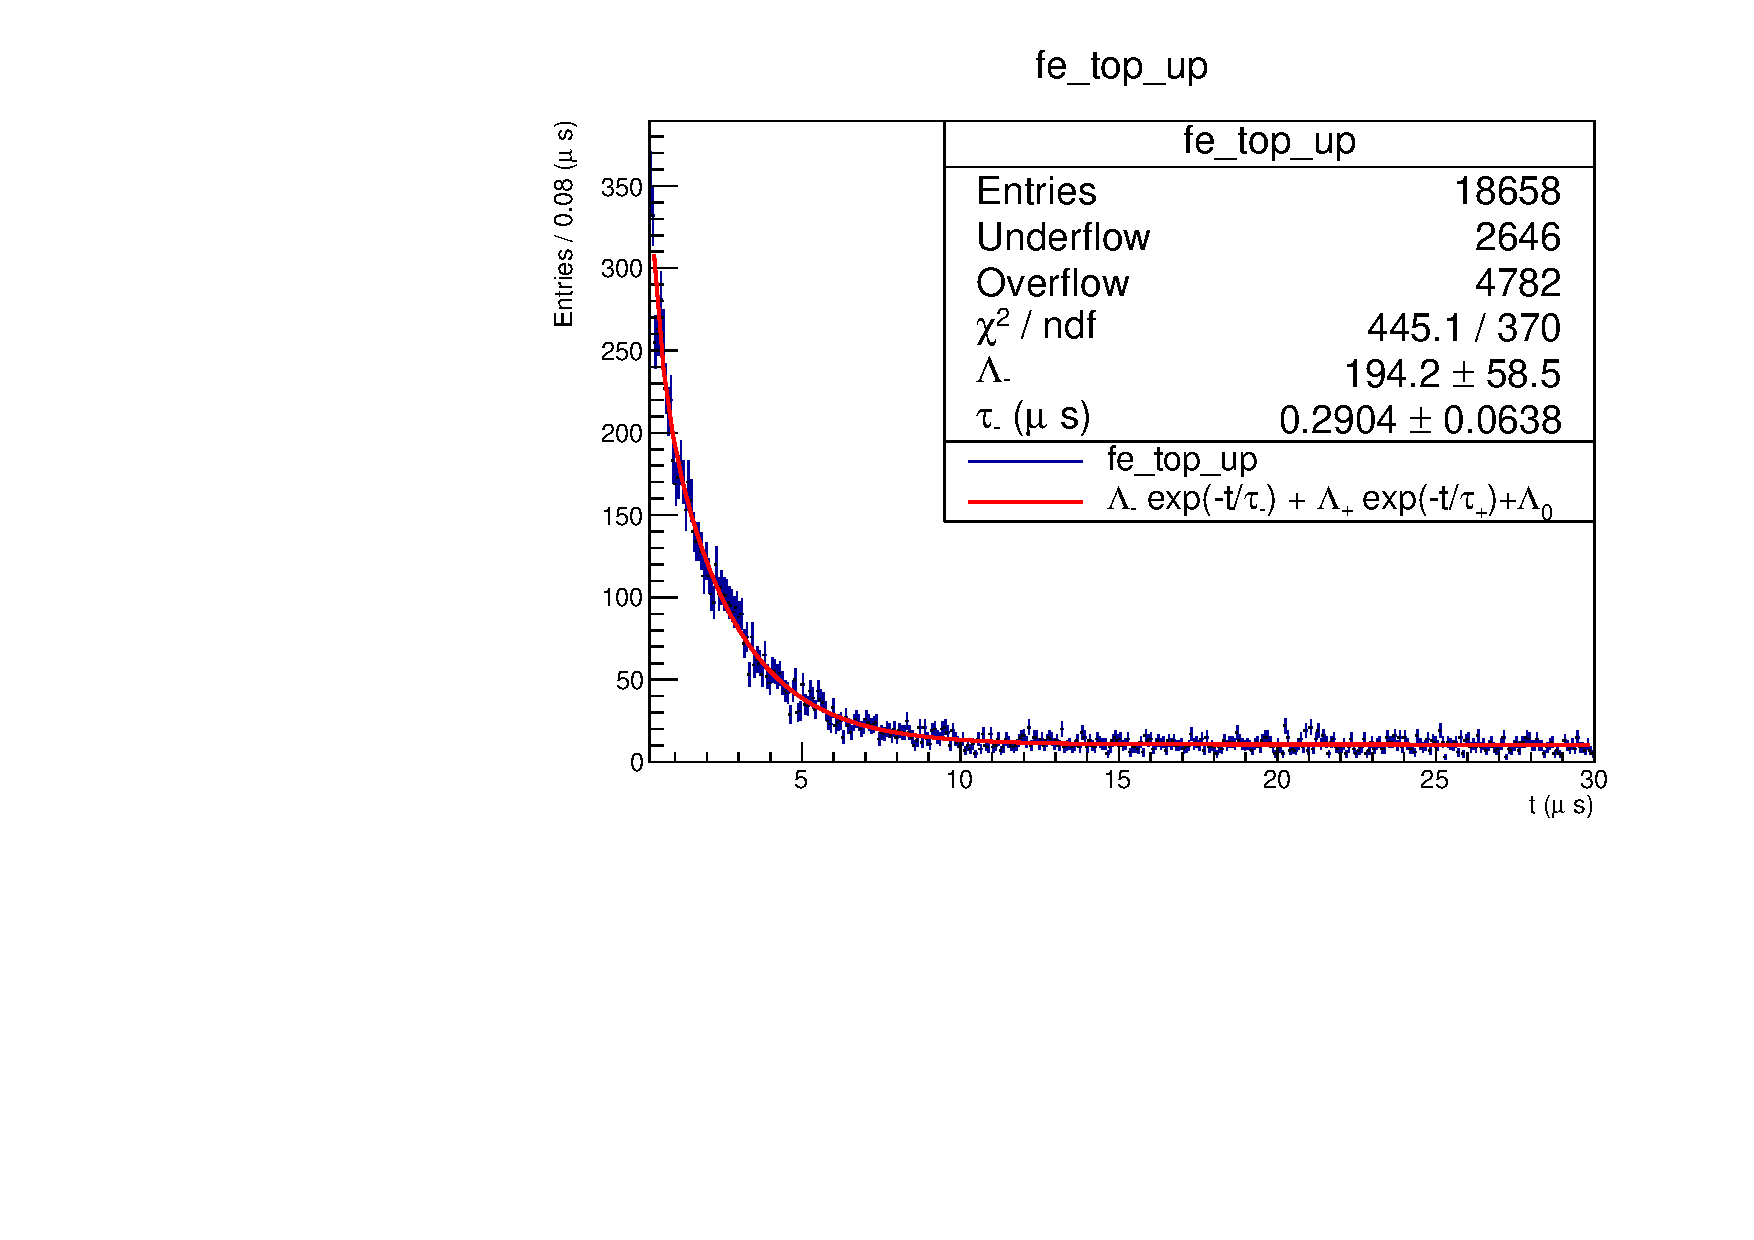
\includegraphics[scale=0.45]{Lab4/Mudecay/fe_top_up_tot.pdf} 
\label{FEUP-}
\end{figure}

\begin{figure}[h!]
\centering
\caption{Time distribution of Fe TOP DOWN fitted in the range [0.185, 30] $\mu s$. [10-11-12-17-19-26/05/22]}
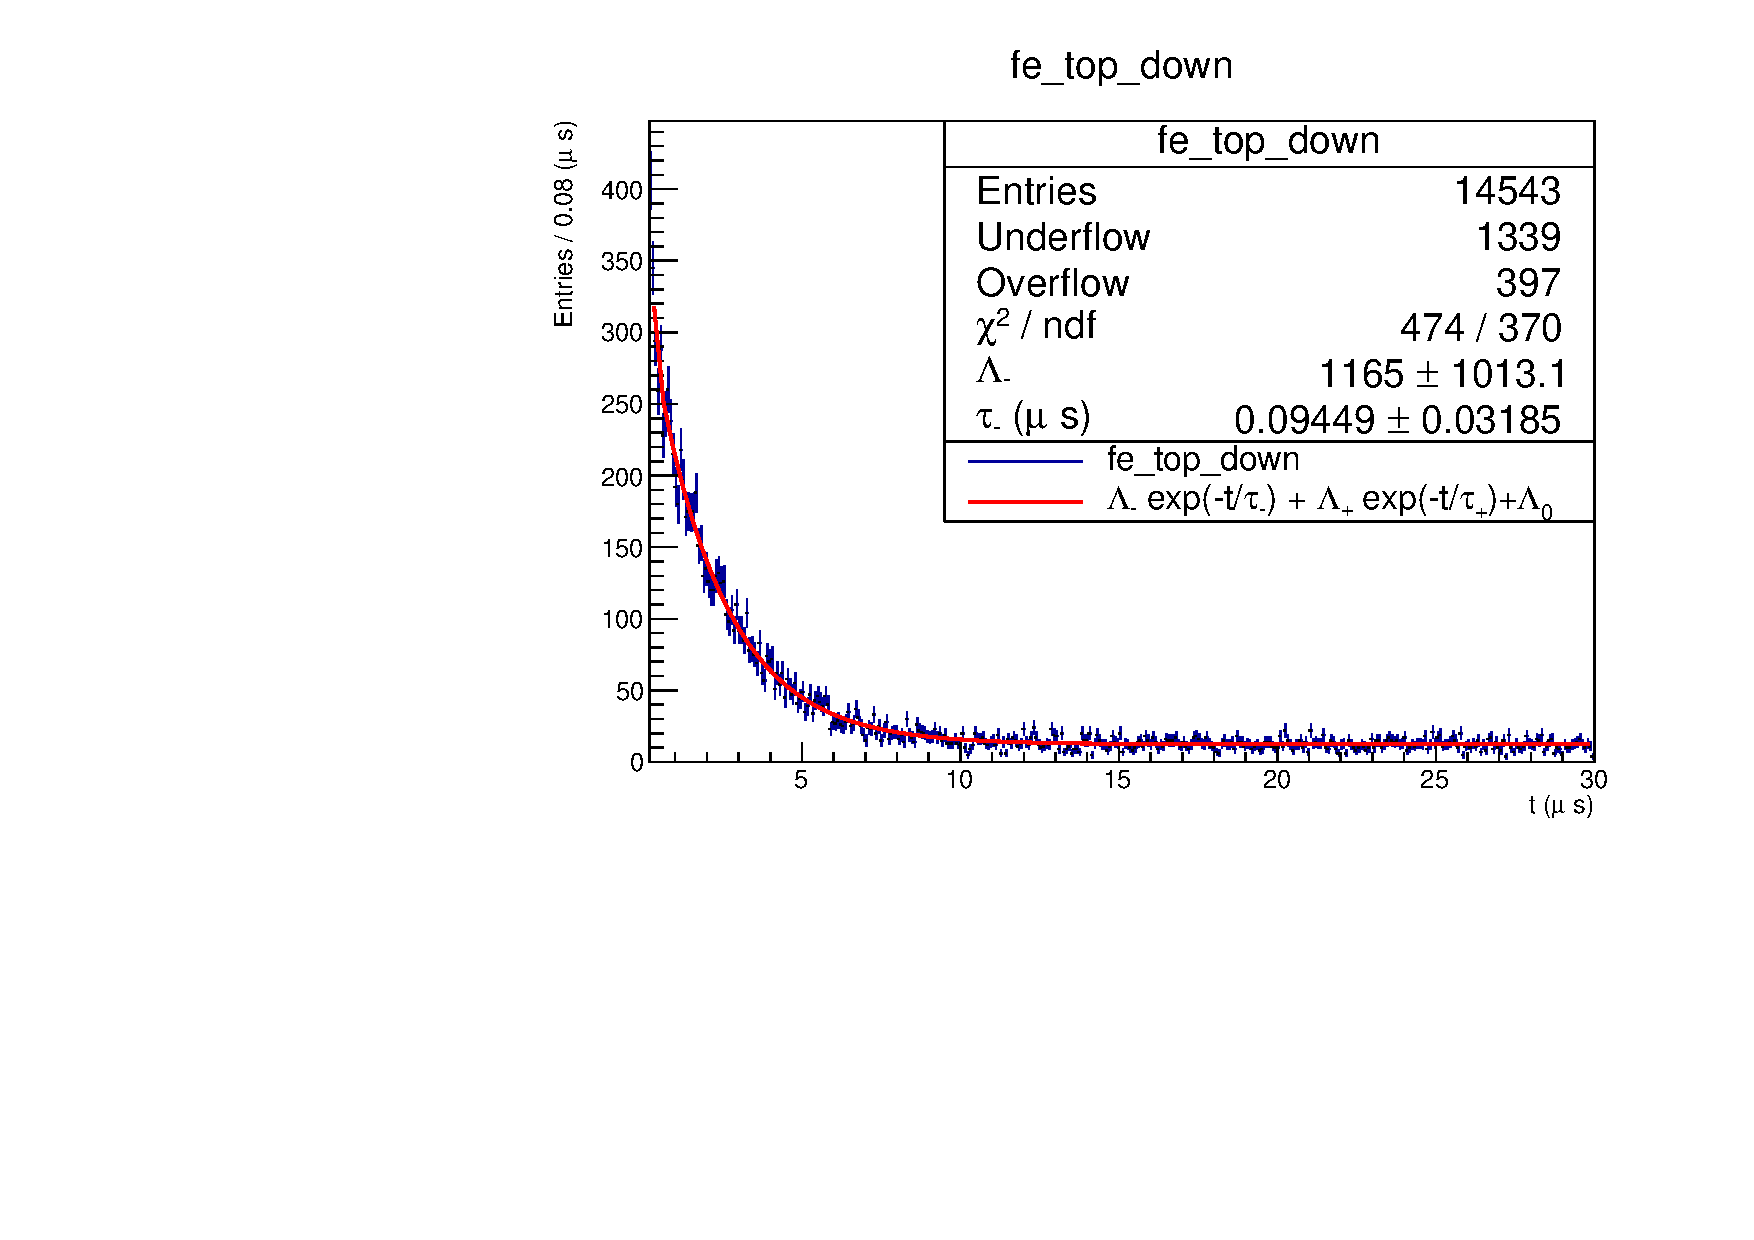
\includegraphics[scale=0.45]{Lab4/Mudecay/fe_top_down_tot.pdf} 
\label{FEDW-}
\end{figure}

The estimates of $\tau_-$ obtained from the two fits are
$\tau_-^{UP}=0.29 \pm 0.06 \text{ (stat)} \pm 0.02 \text{ (syst) }\mu$s and $\tau_-^{DOWN}=0.09 \pm 0.03 \text{ (stat)} \pm 0.01 \text{ (syst) }\mu$s. $\tau_-^{UP}$ is compatible with the expected value ($0.201 \pm 0.004 \mu$s) within just over one standard deviation but $\tau_-^{DOWN}$ is not compatible neither with the expected value nor with the other measurement within 3 standard deviations. In order to test if the null hypothesis of $\tau_- = 0.201$ is to be excluded from the DOWN data set, another fit was performed with $\tau_-$ fixed to the expected value and the $\chi^2$ of this fit was confronted with the one of the previous fit. The results yield $\chi^2_{free} = 474$ when the parameter is left free and $\chi^2_{fix} = 480$ when fixed. 

These $\chi^2$ are the values of the GOF statistics 

\begin{equation}
   \chi^2=2\log\frac{\prod_i Poiss(k_i;k_i)}{\text{sup}L} 
\end{equation}


where $k_i$ are the counts in each bin $i$ and $L$ is the likelihood of the model in question. 
\\
By taking the difference between the $\chi^2$ of the two fits with the two models one obtains a variable 

\begin{equation}
    \Delta \chi^2=2\log \frac{\text{sup}L_{free}}{\text{sup}L_{fix}}
\end{equation}

this variable is distributed (Wilk's theorem), in the null hypothesis $L_{fix}$, as a $\chi^2$ with a number of DOF equal to the difference of the free parameters of the two models. This is thanks to the fact that the two models are one a subcase of the other ($\tau_-$ fixed). \footnote{It actually also requires that, when not under $H_0$, the pivotal quantity tends to have either values bigger or smaller than under $H_0$} In this case the DOF are 1.
This difference found is equal to 6 which, for a $\chi^2_1$, has a p-value of 0.014. This rejects the null hypothesis of $\tau_-$ being equal to its tabulated value with a significance of $\alpha=0.05$. 

\subsection{$\tau_-$ in Al}
The fits UP and DOWN when using Al are shown in Figure \ref{ALUP-} \ref{ALDW-}. 

\begin{figure}[h!]
\centering
\caption{Time distribution of Al BOT UP fitted in the range [0.4, 30] $\mu s$. [19-26/05/22]}
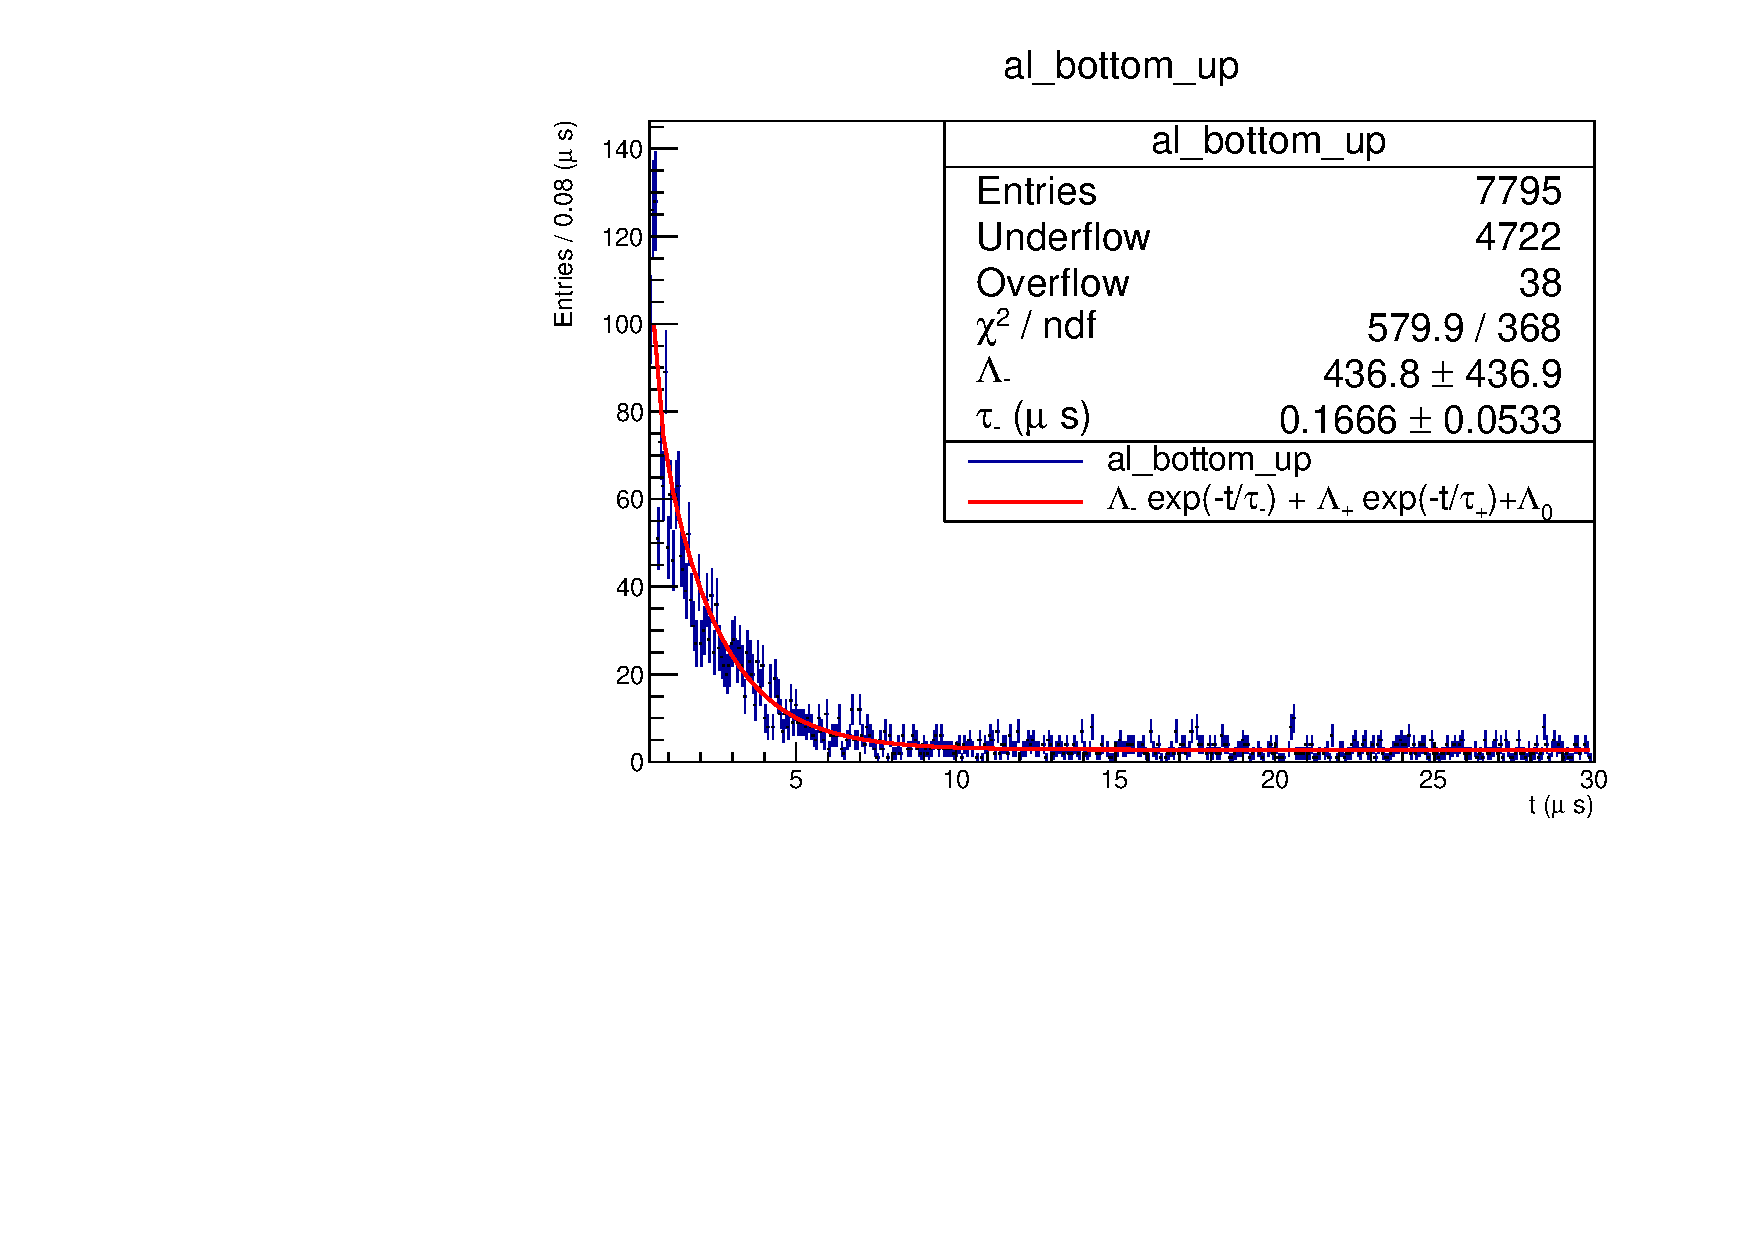
\includegraphics[scale=0.45]{Lab4/Mudecay/al_bottom_up_tot.pdf} 
\label{ALUP-}
\end{figure}

\begin{figure}[h!]
\centering
\caption{Time distribution of Al BOT DOWN fitted in the range [0.4, 30] $\mu s$. [19-26/05/22]}
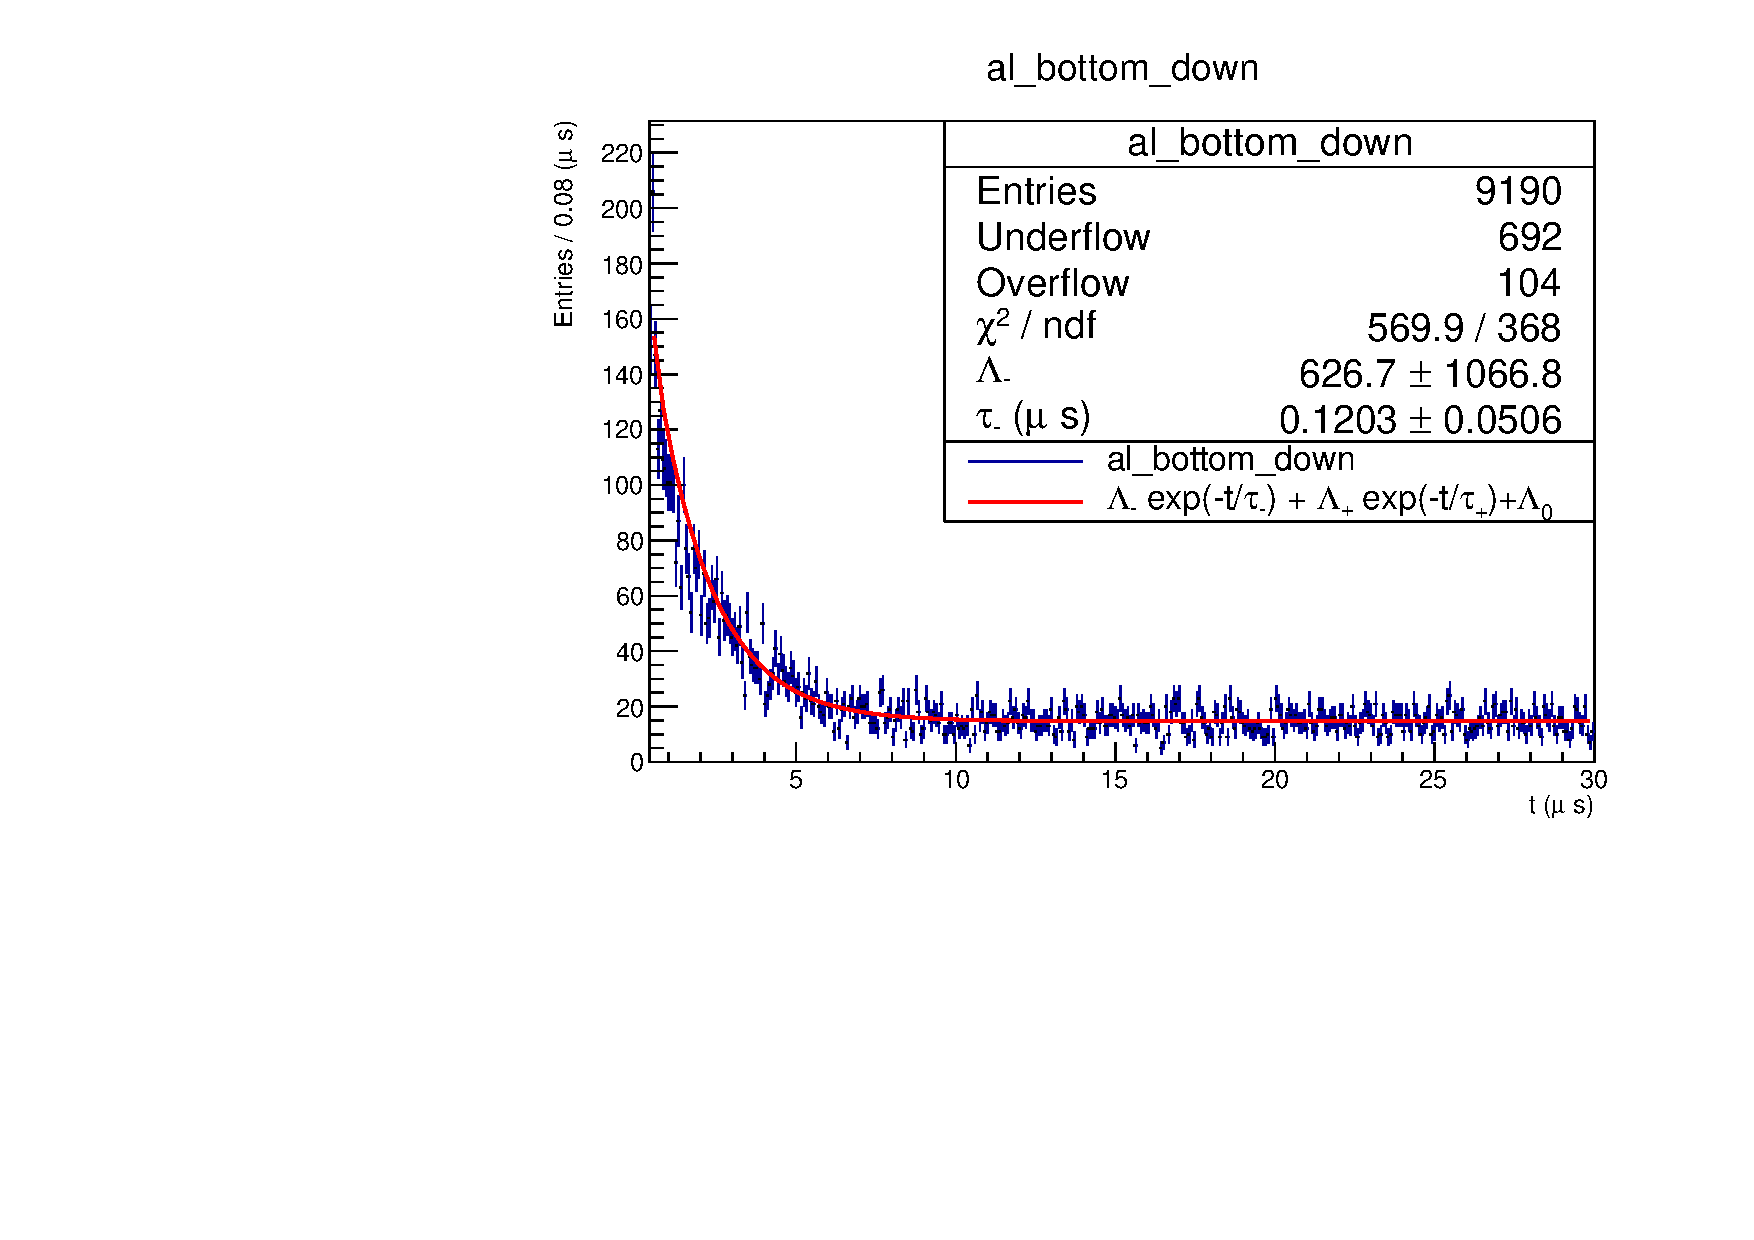
\includegraphics[scale=0.45]{Lab4/Mudecay/al_bottom_down_tot.pdf} 
\label{ALDW-}
\end{figure}

The fits yield $\tau_-^{UP}=0.17 \pm 0.05 \text{ (stat)} \pm 0.02 \text{ (syst) }\mu$s and $\tau_-^{DOWN}=0.12 \pm 0.05 \text{ (stat)} \pm 0.01 \text{ (syst) }\mu$s which are not compatible with the expected value ($0.88 \pm 0.01 \mu$s) by more than 10 standard deviations. As explained above a hypothesis test is performed and the results are:
$\chi^2_{UP free}  = 580$ and $\chi^2_{UP fixed}  = 590$, 
$\chi^2_{DOWN free} = 570$ and $\chi^2_{DOWN fixed} = 570$.
\\
These correspond to the p-values $\simeq0.002$ and $\simeq$1 respectively. In the first case the null hypothesis can be rejected witch $\alpha=0.05$, while in the second the data do not contradict the hypothesis that $\tau_-^{Al}=0.88 \mu$s.

\subsection{$\tau_-$ in NaCl}
The TOP and BOT configurations for NaCl (Figure \ref{NACLTOPUP-} \ref{NACLTOPDW-} \ref{NACLBOTUP-} \ref{NACLBOTDW-}) yield $\tau_-^{TOP UP} =  0.5\pm 0.1 \text{ (stat)} \pm 0.1 \text{ (syst) }\mu$s, $\tau_-^{TOP DOWN} = 0.7\pm 0.2 \text{ (stat)} \pm 0.02 \text{ (syst) }\mu$s and $\tau_-^{BOT DOWN} = 0.7\pm 0.1 \text{ (stat)} \pm 0.01 \text{ (syst) }\mu$s are compatible within just one standard deviation with the expected value ($\sim 0.7 \mu$s), while $\tau_-^{BOT UP} =  0.26\pm 0.03 \text{ (stat)} \pm 0.04 \text{ (syst) }\mu$s is more than 5 standard deviations from it. Since 
$\chi^2_{BOT \, UP \, free} = 695$ and $\chi^2_{BOT \, UP \, fixed} = 747$, the $\Delta \chi^2$ gives a p-value less than 0.0001.

\begin{figure}[h!]
\centering
\caption{Time distribution of NaCl TOP UP fitted in the range [0.25, 30] $\mu s$. [18-19-24/05/22]}
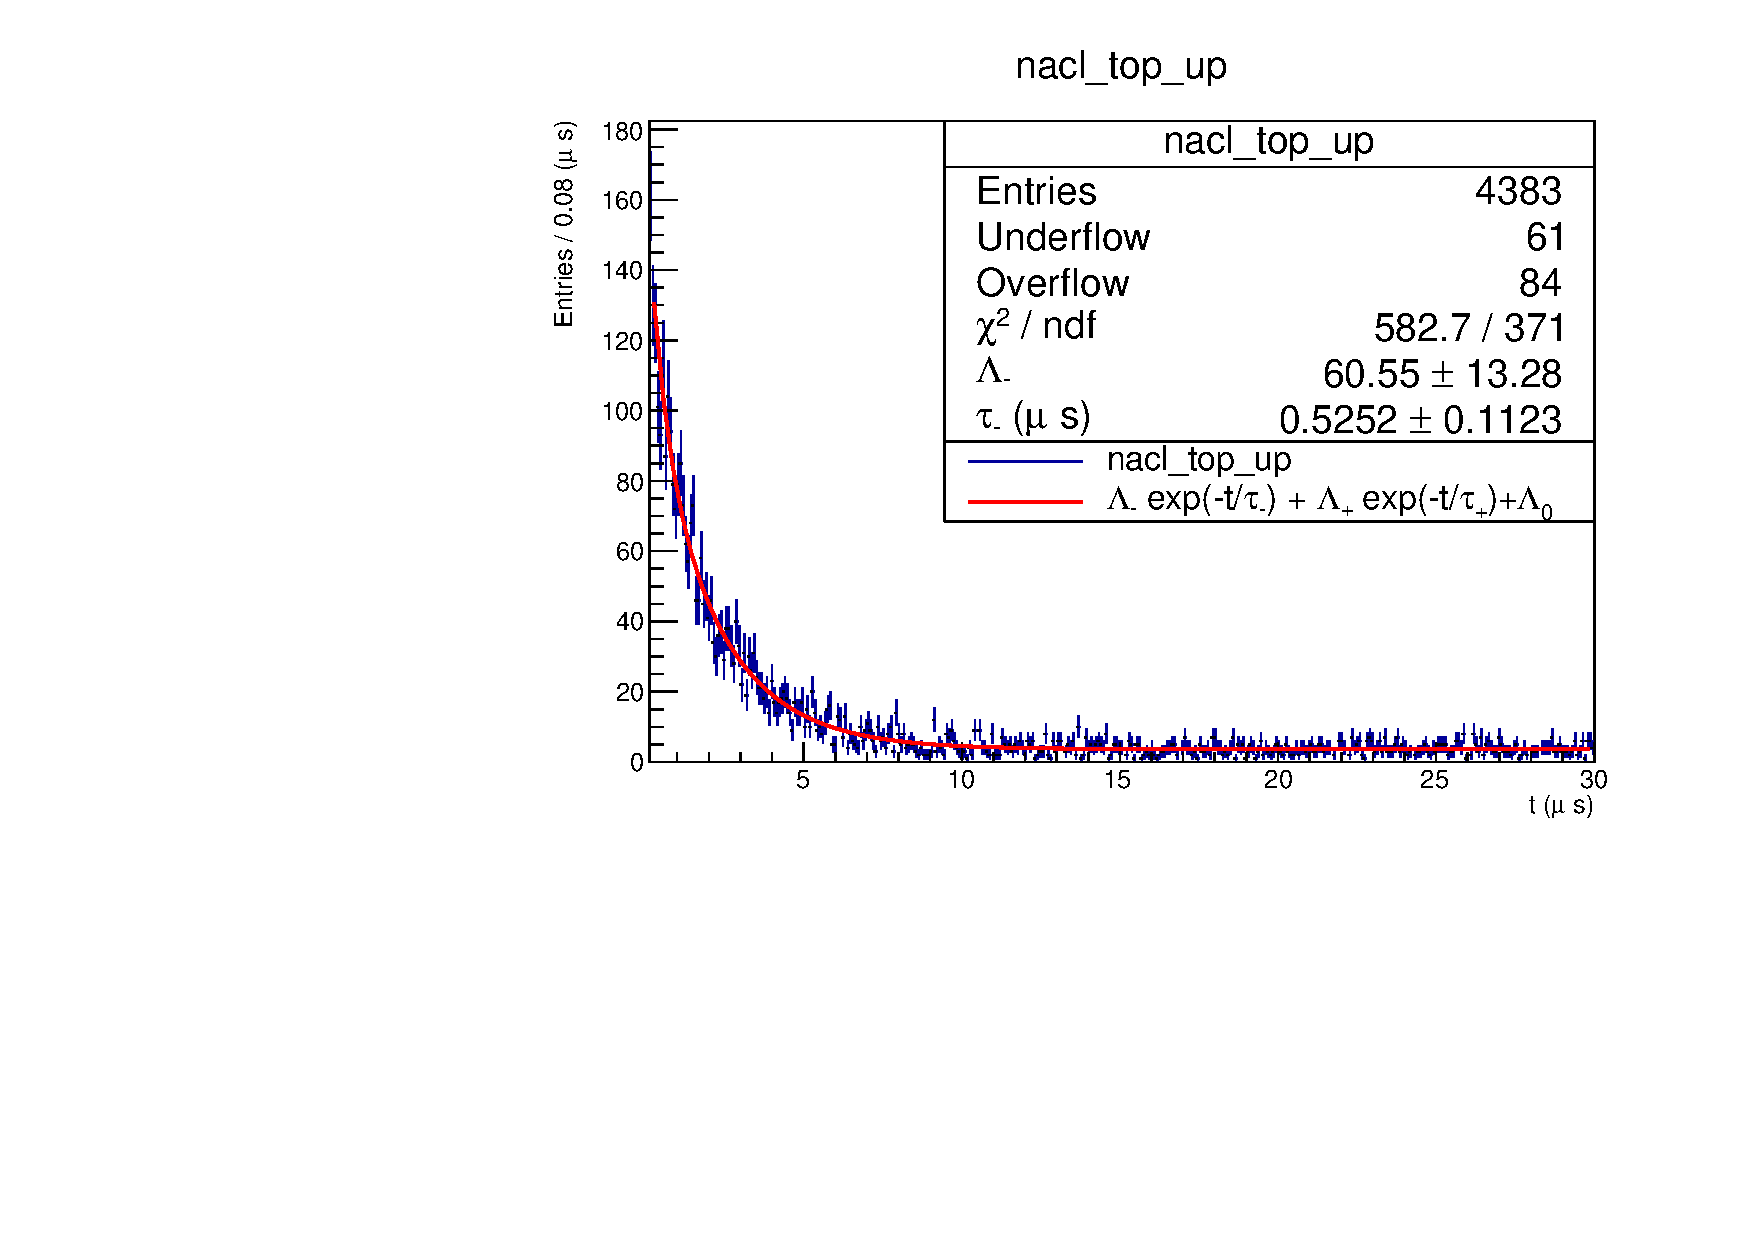
\includegraphics[scale=0.45]{Lab4/Mudecay/nacl_top_up_tot.pdf} 
\label{NACLTOPUP-}
\end{figure}

\begin{figure}[h!]
\centering
\caption{Time distribution of NaCl TOP DOWN fitted in the range [0.25, 30] $\mu s$. [18-19-24/05/22]}
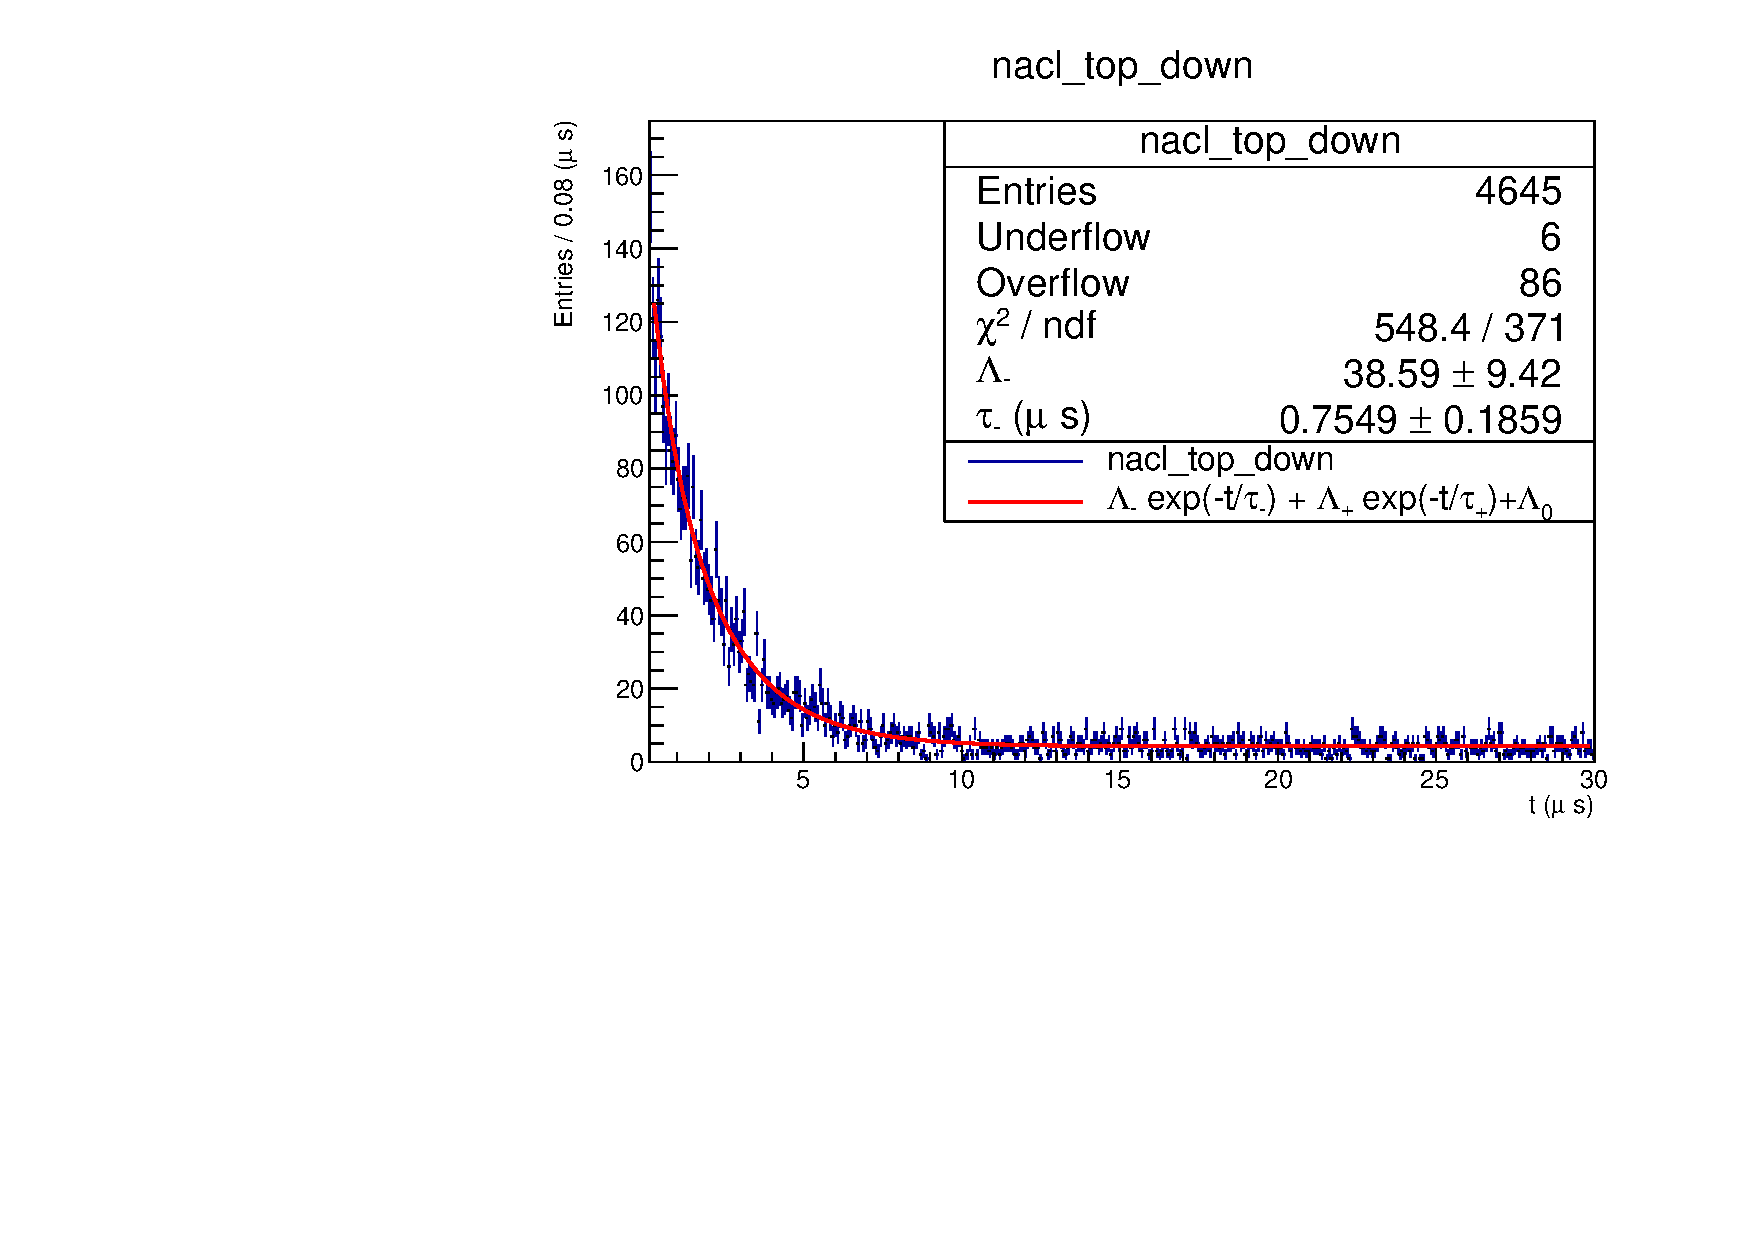
\includegraphics[scale=0.45]{Lab4/Mudecay/nacl_top_down_tot.pdf}
\label{NACLTOPDW-}
\end{figure}

\begin{figure}[h!]
\centering
\caption{Time distribution of NaCl BOT UP fitted in the range [0.25, 30] $\mu s$. [25-26-30/05/22]}
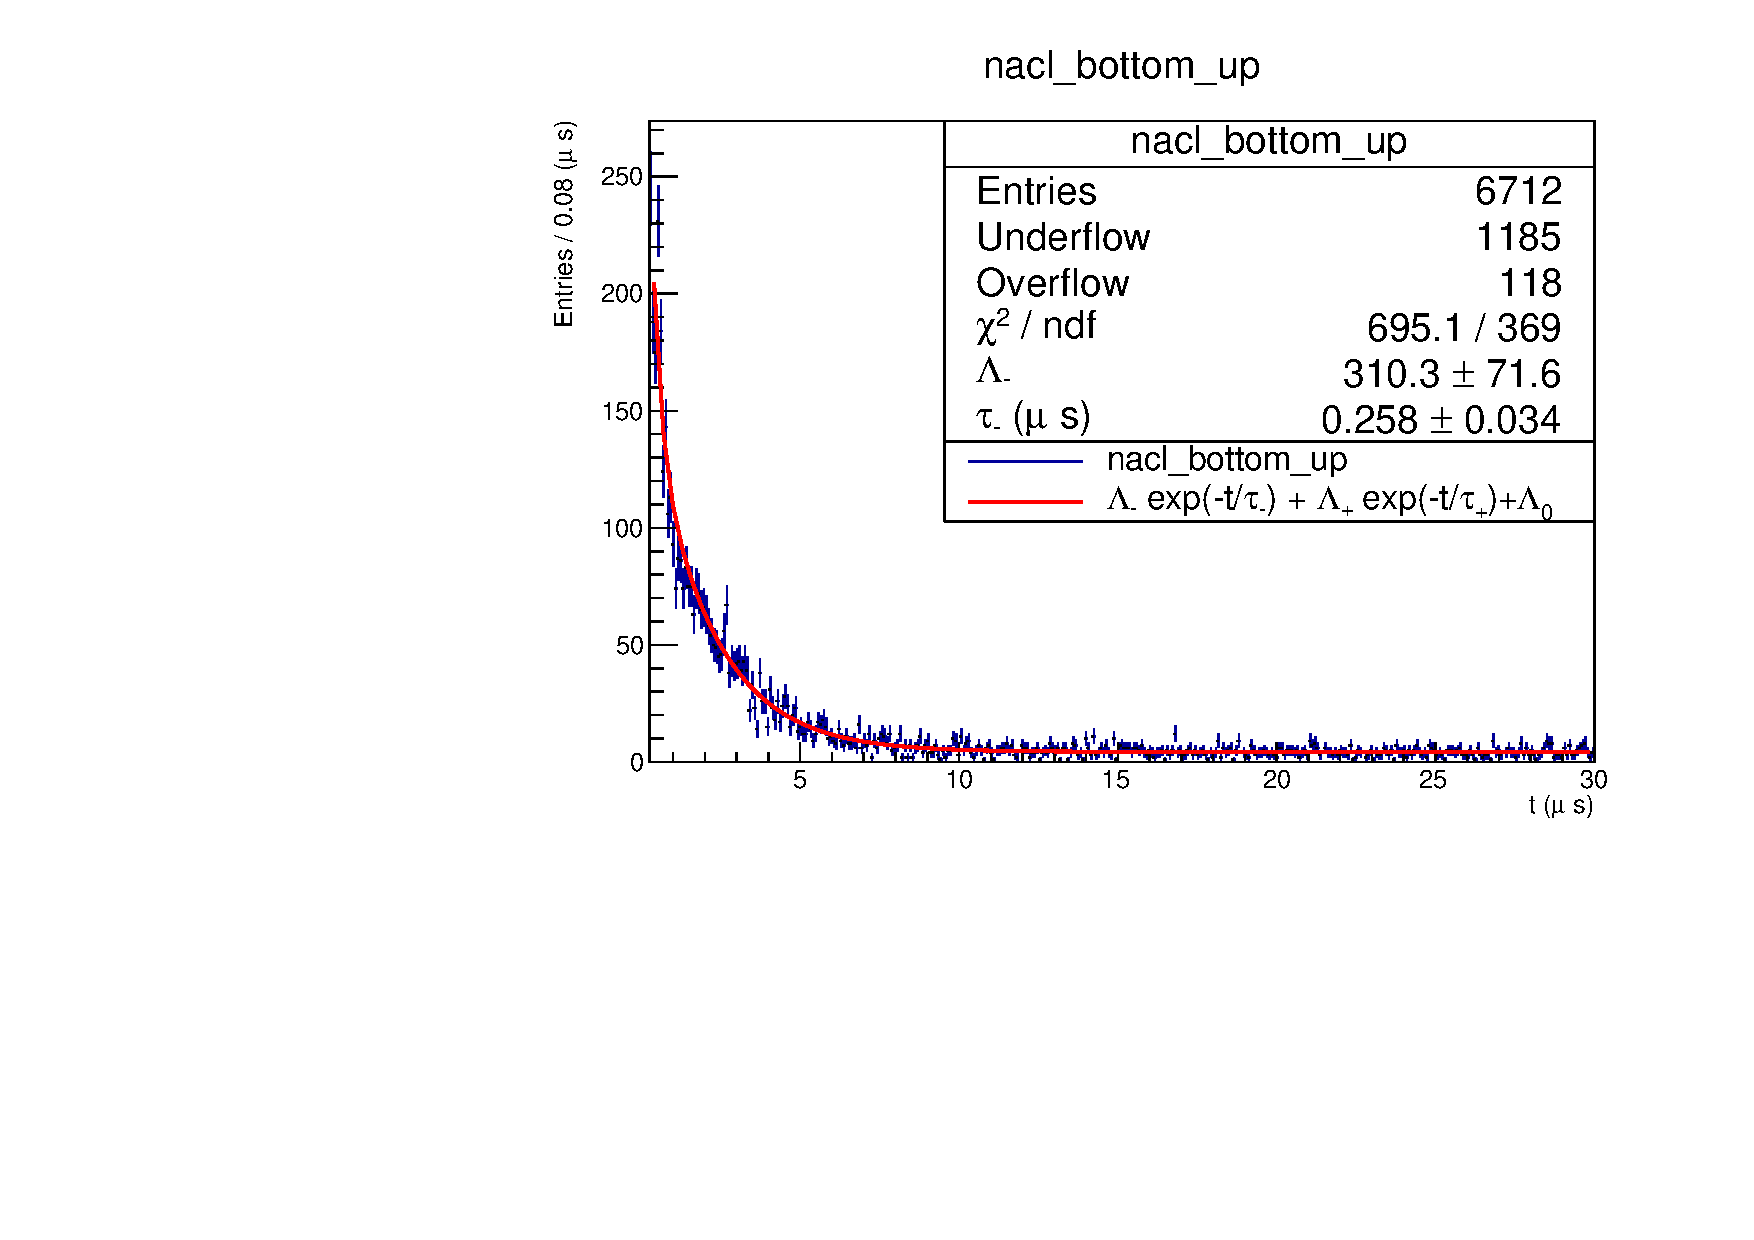
\includegraphics[scale=0.45]{Lab4/Mudecay/nacl_bottom_up_tot.pdf} 
\label{NACLBOTUP-}
\end{figure}

\begin{figure}[h!]
\centering
\caption{Time distribution of NaCl BOT DOWN fitted in the range [0.25, 30] $\mu s$. [25-26-30/05/22]}
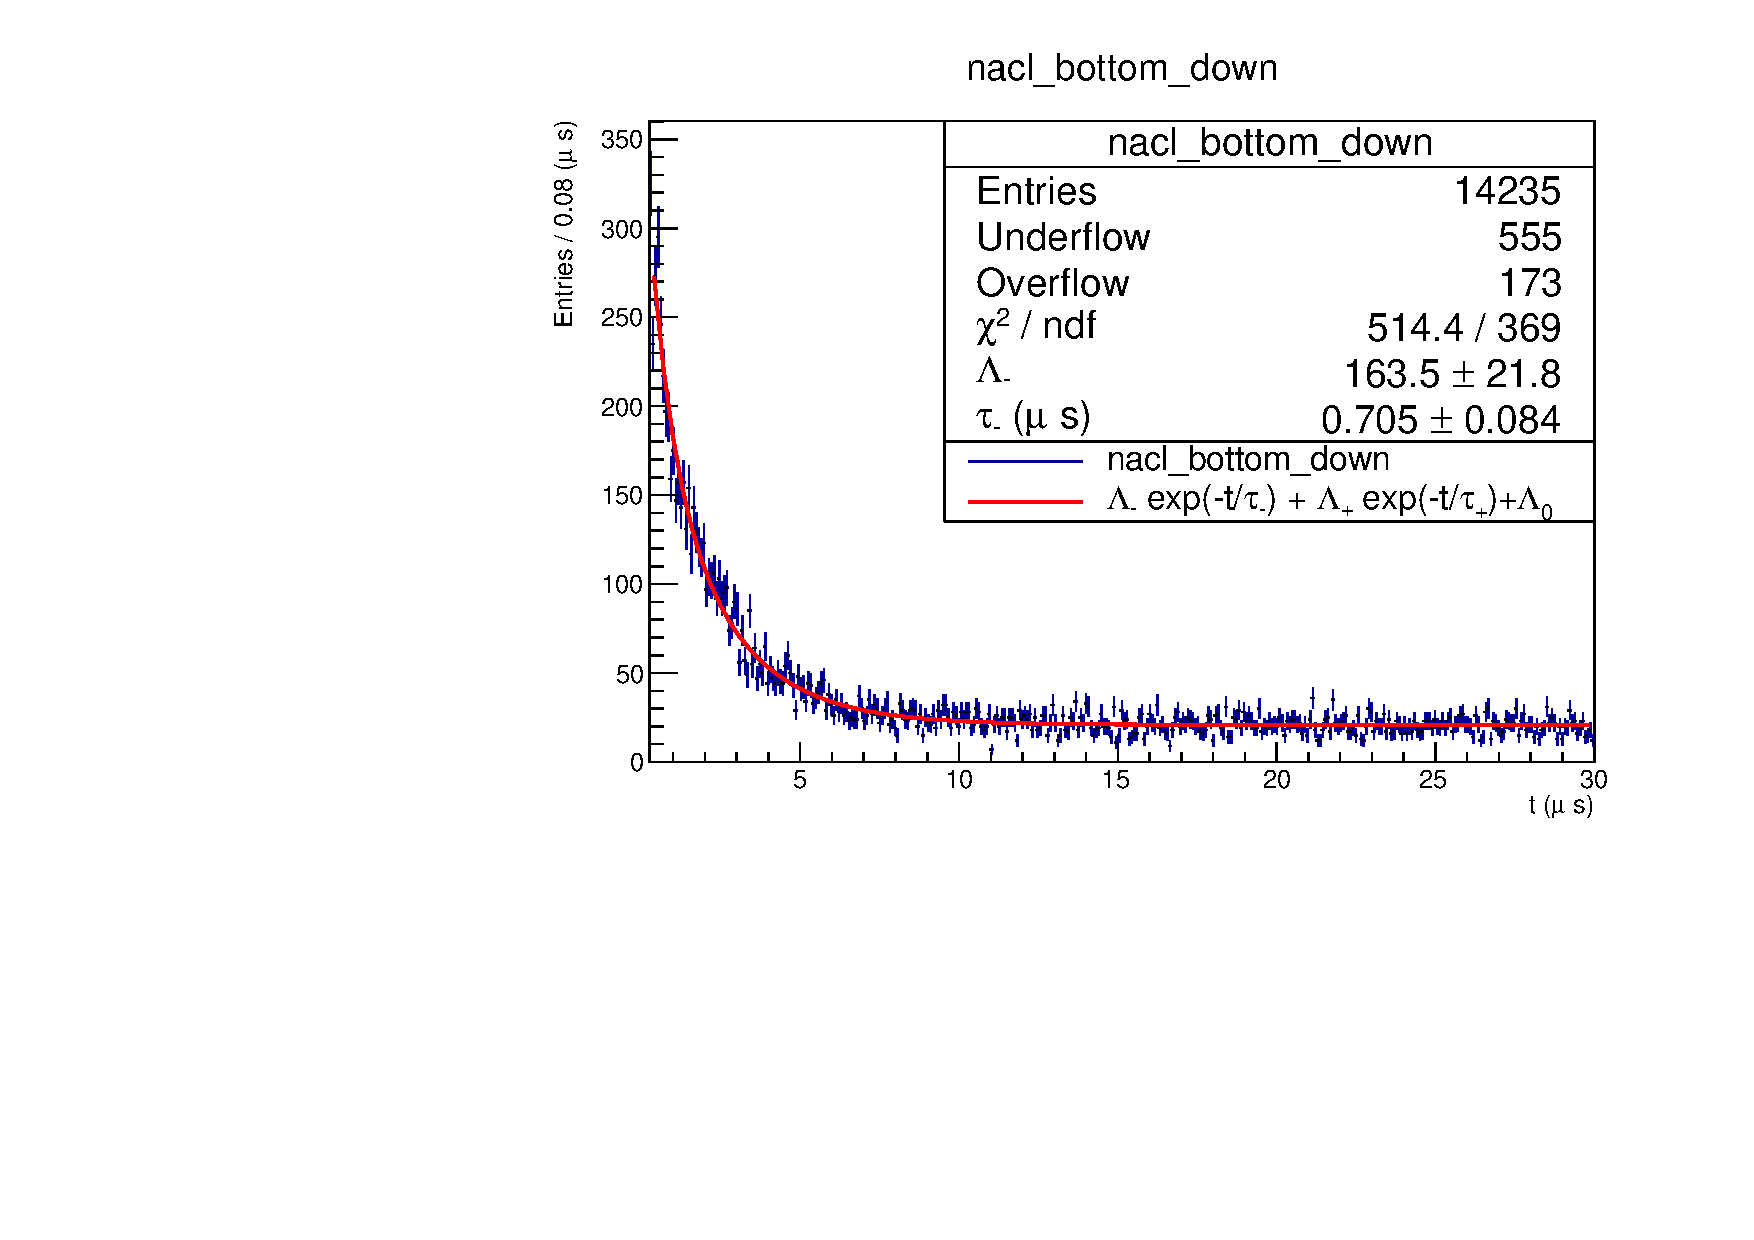
\includegraphics[scale=0.45]{Lab4/Mudecay/nacl_bottom_down_tot.pdf} 
\label{NACLBOTDW-}
\end{figure}


\subsection{$\tau_-$ in Mag Fe}
When using the magnetic circuit, the measurement is done in both the TOP and BOT sections (Figure \ref{MAGTOPUP-} \ref{MAGTOPDW-} \ref{MAGBOTUP-} \ref{MAGBOTDW-}). The different results show that 
\begin{align*}
    \tau_-^{TOP UP} & =  0.25\pm 0.03 \text{ (stat)} \pm 0.04 \text{ (syst) }\mu \text{s} \\
        \tau_-^{BOT UP} &= 0.18\pm 0.02 \text{ (stat)} \pm 0.01 \text{ (syst) }\mu \text{s}\\
        \tau_-^{BOT DOWN} &= 0.29\pm 0.03 \text{ (stat)} \pm 0.01 \text{ (syst) }\mu\text{s}\\
        \tau_-^{TOP DOWN} &=  0.10\pm 0.09 \text{ (stat)} \pm 0.01 \text{ (syst) }\mu\text{s}\\
\end{align*}

These are compatible within a few standard deviation with the expected value ($0.201 \pm 0.004 \mu$s).



\subsection{Possible systematic errors}

There are a few factors that can influence the outcome of the measurements just described, making them incompatible with what is expected.
\\
First, it could be due to a non negligible contribution of the metal bars that support the detector rack. These should be considered now that the fits reach low $t$, but that is not easy to do since it would again force a double exponential fit, which doesn't converge well.
\\
\\
Another reason for the discrepancies of the short lifetimes at low $t$ could be a systematic error due to the presence of afterpulse peaks (e.g. the one at 550-600 ns), that slightly change the pdf but just enough to make the fit converge on a "wrong" conclusion. This could be taken care of in the future by either coming up with a way to subtract the peak or by iterating multiple fits and rescaling the peak region with the fitted function every time, until the peak flattens out.

\begin{figure}[h!]
\centering
\caption{Time distribution of Mag Fe TOP UP fitted in the range [0185, 30] $\mu s$. [25-26-30/05/22]}
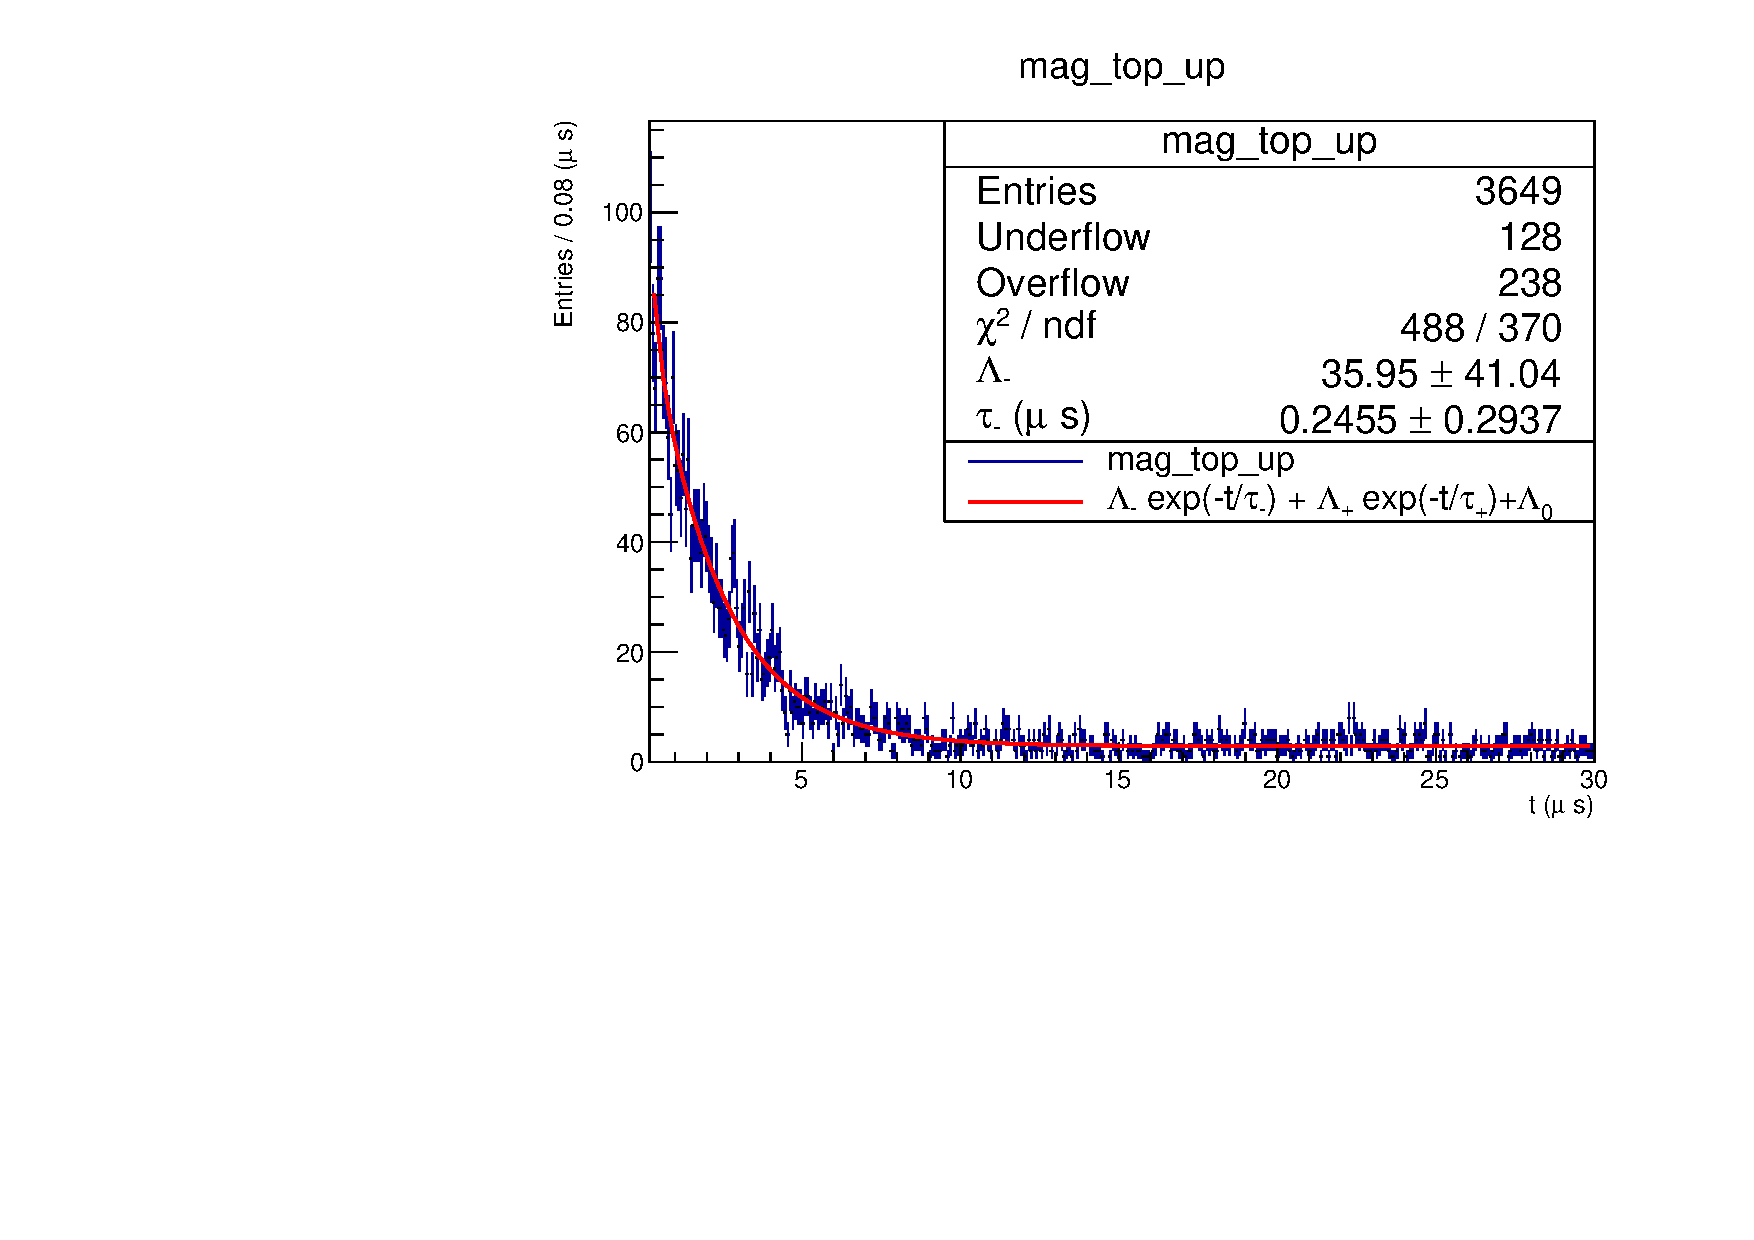
\includegraphics[scale=0.45]{Lab4/Mudecay/mag_top_up_tot.pdf} 
\label{MAGTOPUP-}
\end{figure}

\begin{figure}[h!]
\centering
\caption{Time distribution of Mag Fe TOP DOWN fitted in the range [0.185, 30] $\mu s$. [25-26-30/05/22]}
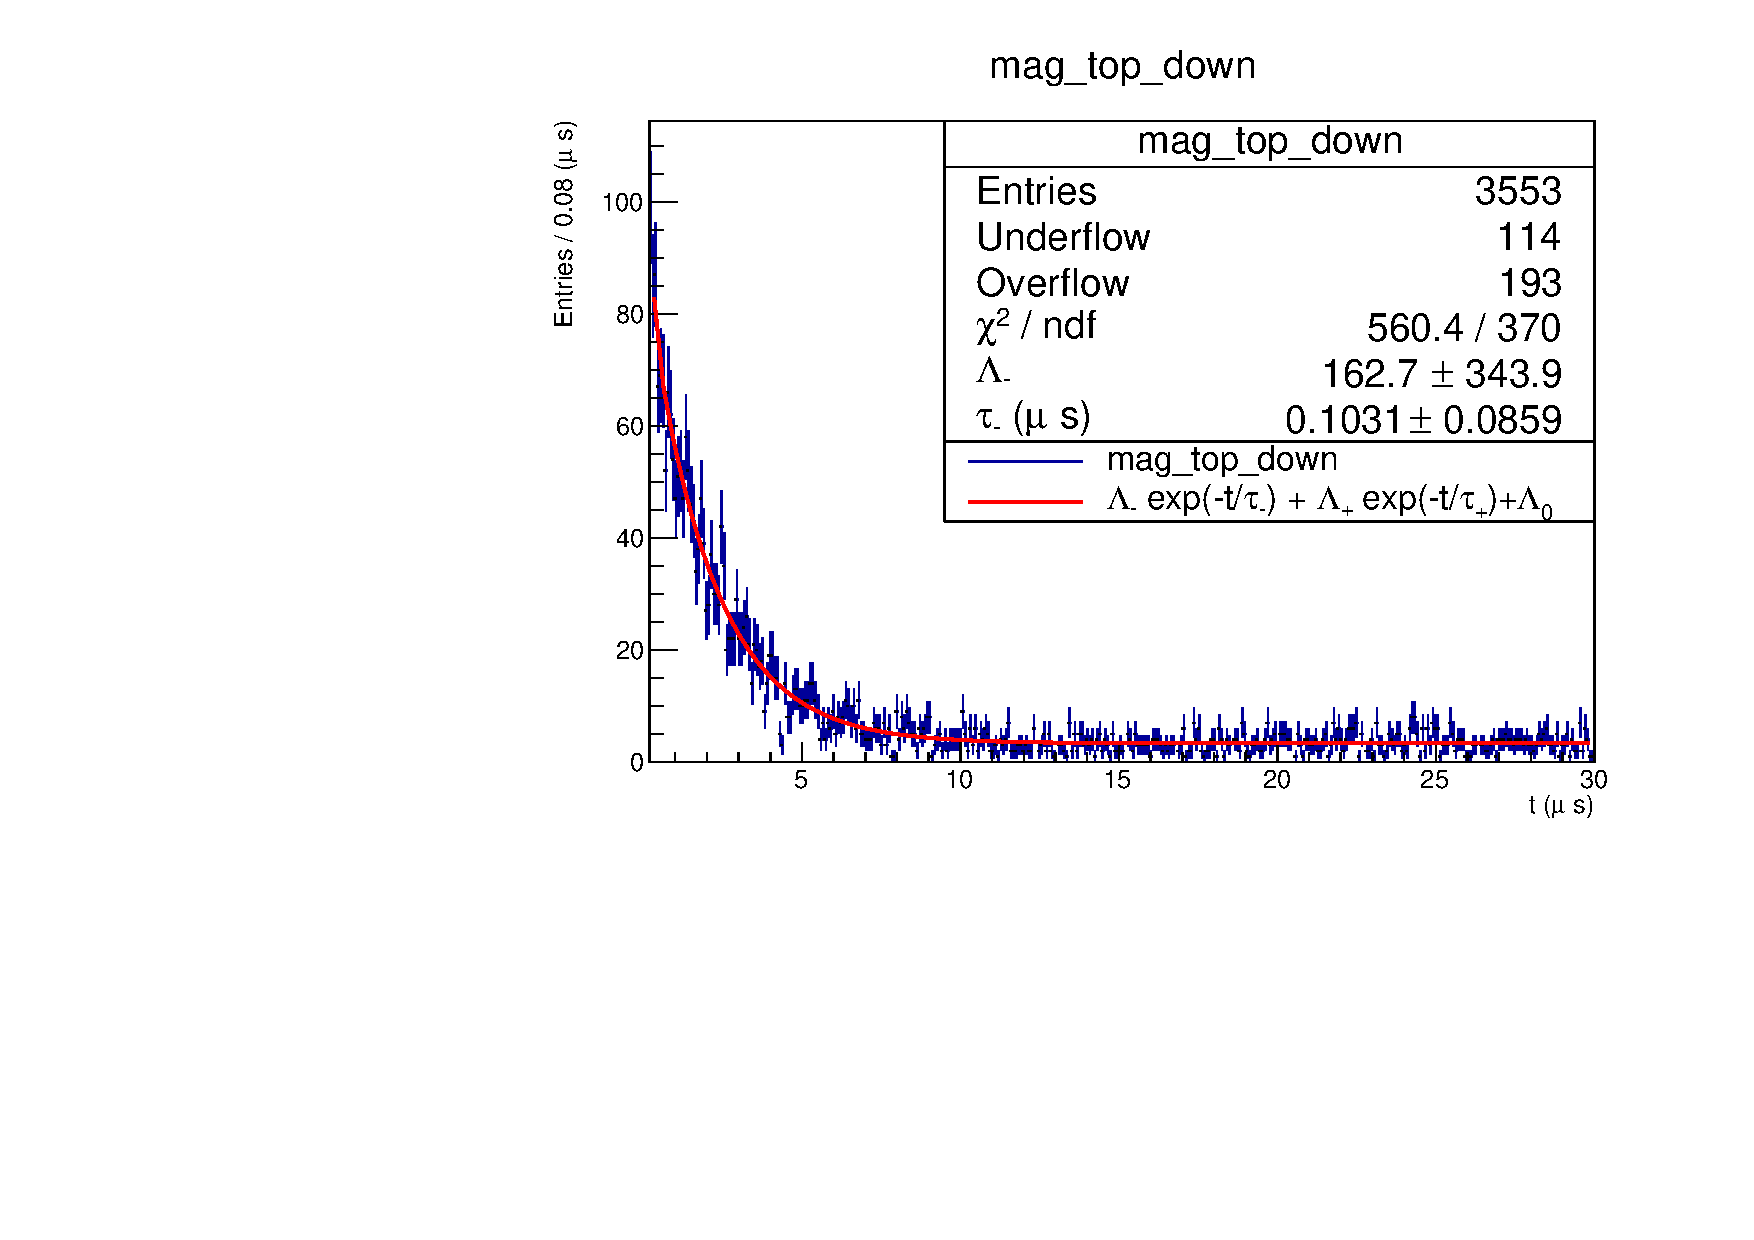
\includegraphics[scale=0.45]{Lab4/Mudecay/mag_top_down_tot.pdf}
\label{MAGTOPDW-}
\end{figure}

\begin{figure}[h!]
\centering
\caption{Time distribution of Mag Fe BOT UP fitted in the range [0.18, 30] $\mu s$. [18-19-24/05/22]}
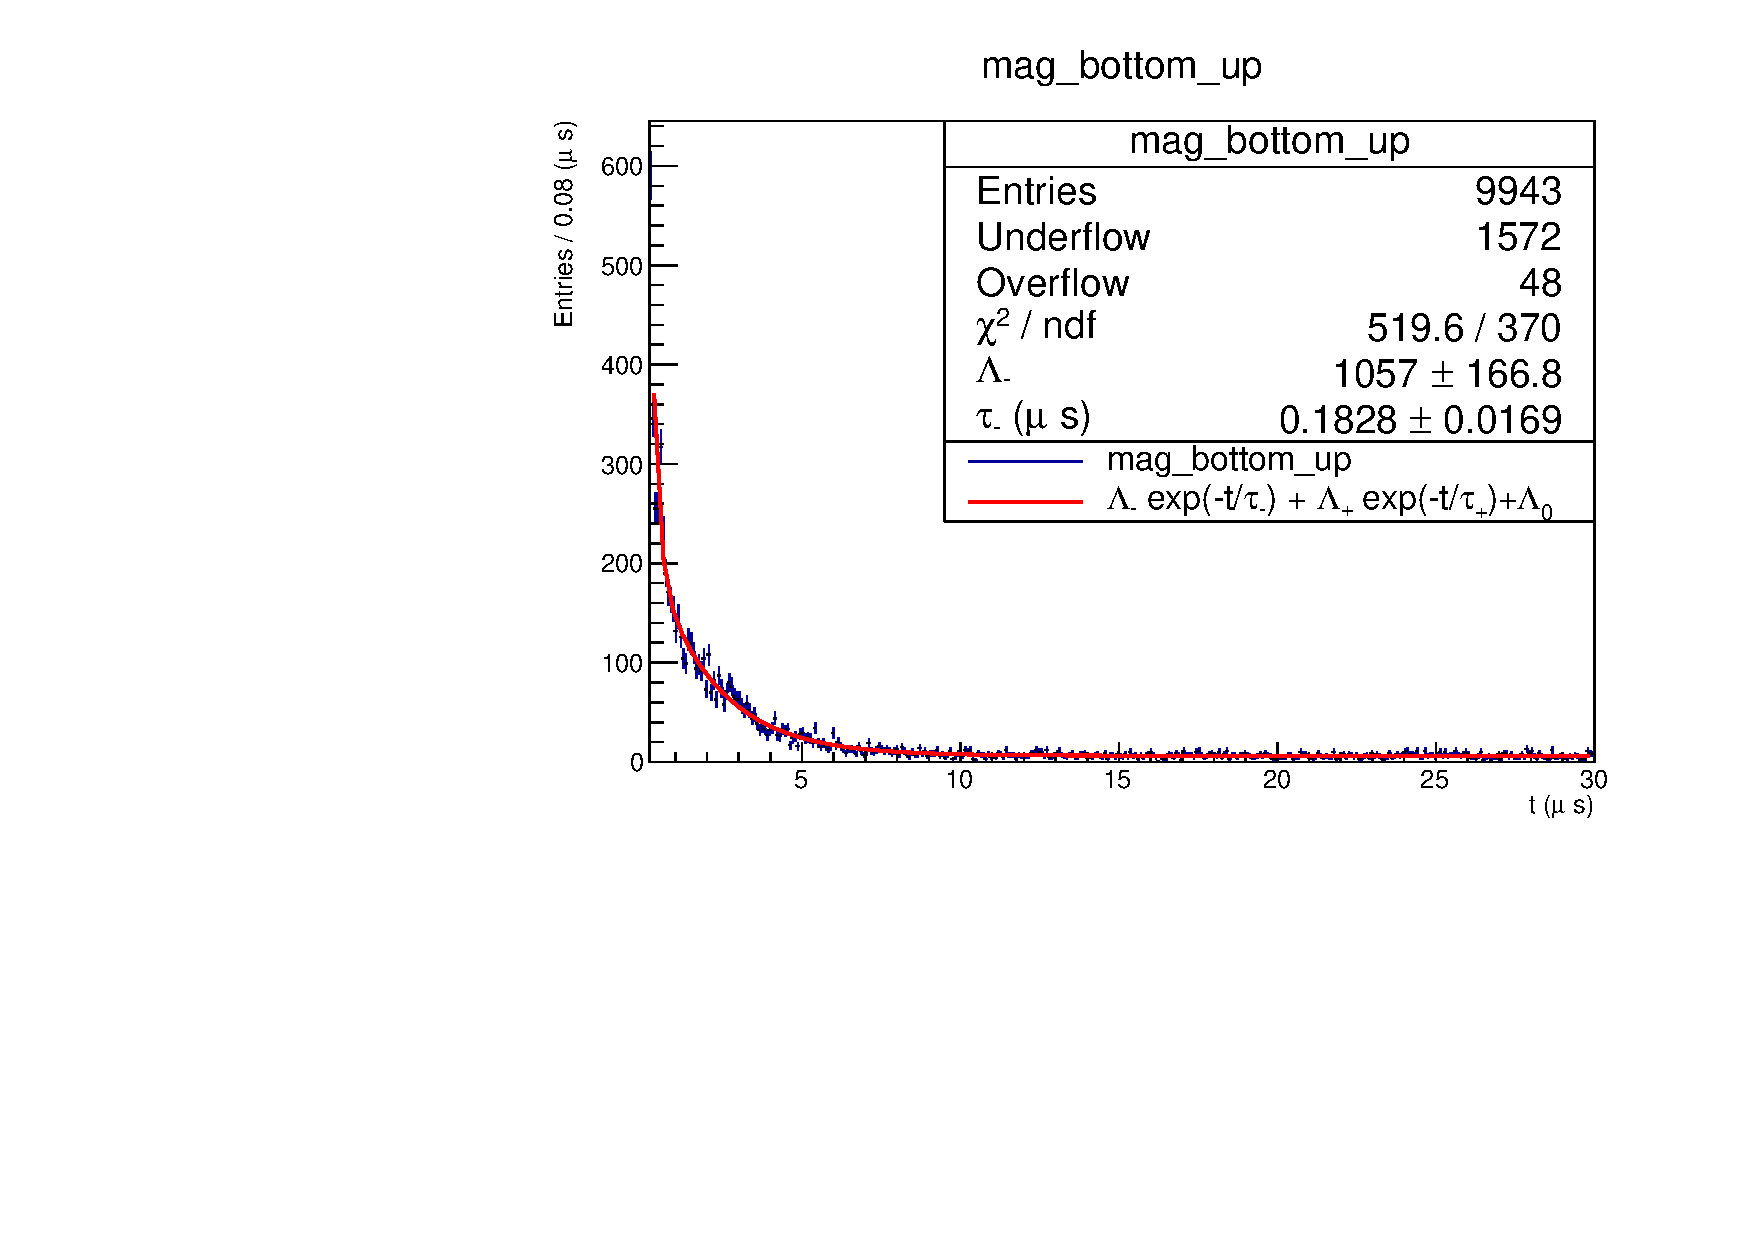
\includegraphics[scale=0.45]{Lab4/Mudecay/mag_bottom_up_tot.pdf}
\label{MAGBOTUP-}
\end{figure}

\begin{figure}[h!]
\centering
\caption{Time distribution of Mag Fe BOT DOWN fitted in the range [0.18, 30] $\mu s$. [18-19-24/05/22]}
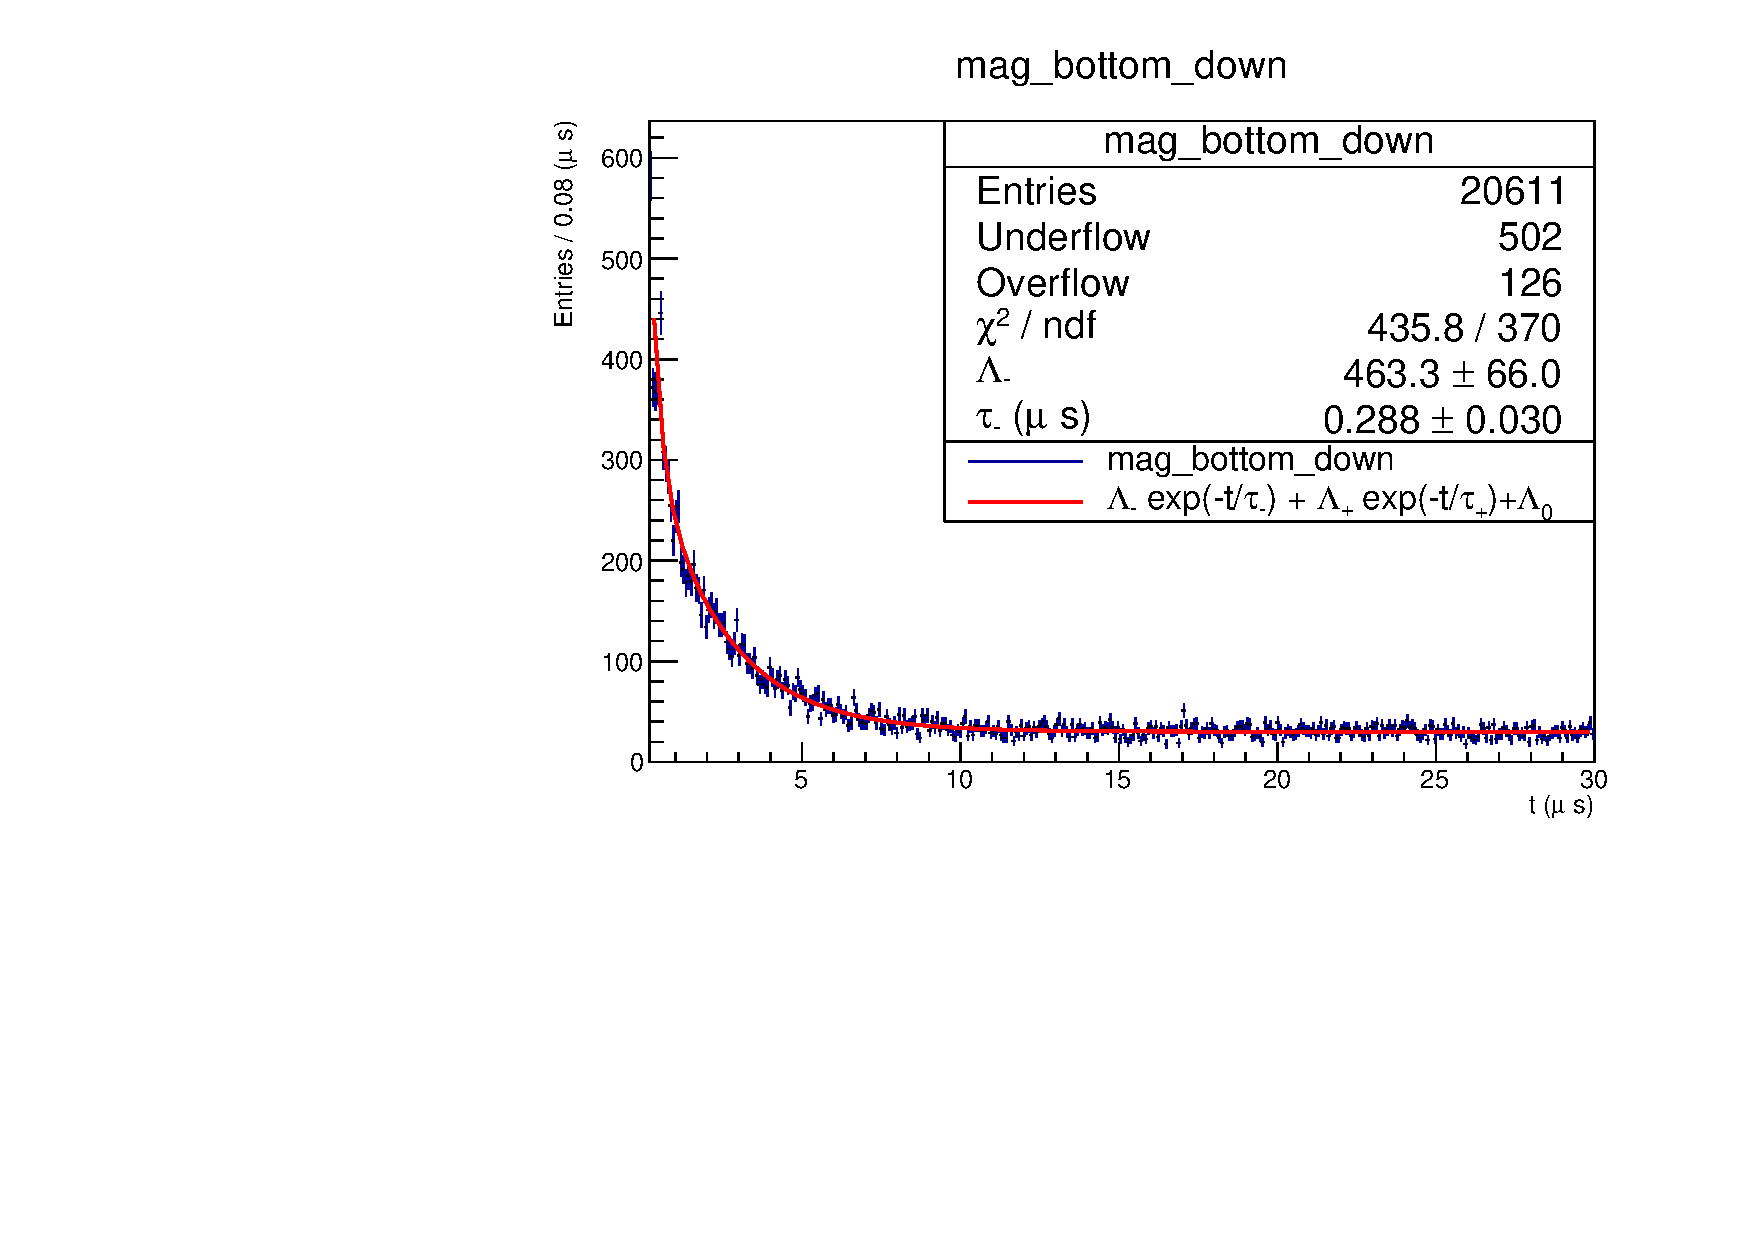
\includegraphics[scale=0.45]{Lab4/Mudecay/mag_bottom_down_tot.pdf} 
\label{MAGBOTDW-}
\end{figure}

\section{Relative Abundances}

In the fitting process not only are the lifetimes are measured, but also the coefficients of the exponential distribution themselves. 

The number of counts of events depends not only on the rate of potential events taking place, but also on the efficiencies of the different detectors. Nonetheless, the data collected for UP (or DOWN) all made use of the same STOP scintillators, regardless of charge of muon. Therefore the \textit{relative} abundance $N^+/N_-$ is independent of the efficiencies of the oscillators. This doesn't however mean that $N^+/N_-=\Lambda_+/\Lambda_-$: efficiencies are not the only potential factor that influences the relative abundance measurement.
\\
As mentioned before, differences in cable lengths bias $t$ with respect to the actual lifetime of the muon by a constant offset. While this systematic shift in the $t$ distribution to the ratio doesn't influence the fitted value of the mean lifetime, it does change the value measured for $\Lambda_\pm$. This change is not the same for the two species, otherwise it could be solved again using $\Lambda_+/\Lambda_-$, but instead depends on the value of the lifetime itself.

\begin{equation}
\label{exposhift}
    \Lambda e^{-(t+t_0)/\tau}\equiv \Tilde{\Lambda}e^{-t/\tau} \quad , \quad \Tilde{\Lambda}=\Lambda e^{-t_0/\tau}\neq \Lambda
\end{equation}

As has been already discussed, however, this shift is too small to influence the fitted values of $\Lambda$, even being a factor of four smaller than the resolution itself.
\\
\\
The results obtained from the various fits of the lifetimes are reported in Table \ref{rel_ab} and are very inconsistent with each other. However, it should be taken into consideration that, when propagating the error on the ratio. the covariance between $\Lambda_+$ and $\Lambda_-$ has not been accounted for. This is because the fit for $\tau_-$ is done in two steps, in one of which the parameter $\Lambda_+$ is fixed, and the \texttt{ROOT} framework doesn't provide the possibility to evaluate the covariance matrix for a fixed parameter. However since they are surely anticorrelated and the function is $\Lambda_+/\Lambda_-$, the propagated errors are certainly underestimated.

\begin{table}[h]
\centering
\begin{tabular}{|c|c|}
\hline
Material & $\Lambda_+/\Lambda_-$ \\
\hline

Fe TOP UP & $1.4 \pm 0.4$ \\
Fe TOP DOWN & $0.3 \pm 0.2$ \\
NaCl TOP UP & $1.7 \pm 0.5$ \\
NaCl TOP DOWN & $2.7 \pm 0.8$ \\
NaCl BOT UP & $0.5 \pm 0.1$ \\
NaCl BOT DOWN & $1.2 \pm 0.2$ \\
Mag BOT UP & $0.21 \pm 0.03$ \\
Mag BOT DOWN & $0.6 \pm 0.1$ \\
\hline
\end{tabular} 
\caption{Relative abundances of $\mu^+$ and $\mu^-$.}
\label{rel_ab}
\end{table}

The results from Fe TOP UP, NaCl TOP UP and NaCl BOT DOWN are compatible with the expected value of 1.27 within one standard deviation, however the other measurements are not compatible. This may be due to the great numerical difficulty in discerning one exponential, and so its coefficient, from the other. This is also evidenced by the great uncertainties of the fitted $\Lambda$s.




\section{Asymmetry in the $\mu$ decay}
Cosmic ray $\mu^{\pm}$ originate in the atmosphere from the reactions: $\pi^{\pm} \rightarrow \mu^{\pm} \nu_{\mu} (\bar{\nu}_{\mu})$. In the pions rest frame the neutrino and the muons are emitted back-to-back. Since $\pi^+$ ($\pi^-$ ) have spin 0 and $\nu$ ($\bar{\nu}$) are \textit{left-handed} (\textit{right-handed}), angular momentum conservation forces $\mu^+$ ($\mu^-$) to be \textit{left-handed} (\textit{right-handed}). This implies that muons and anti-muons arrive to the detector with opposite spins on average, since these are the muons that are emitted more energetically respectively. This is a well documented fact \cite{mupolarized}. However, the amplitude of the $\mu^+$ ( $\mu^-$) decay is maximum when the $e^+$ ($e^-$) momentum is parallel (anti-parallel) to the $\mu^+$ ( $\mu^-$) spin (this asymmetry is causes parity violation in weak decays). This allows for the measurement of asymmetry in the decays since both $\mu^{\pm}$ emit their $e^{\pm}$ upwards (Figure \ref{mudecay}, \textit{even if they arrived with average spins pointing in opposite directions}.


\begin{figure}[h!]
\centering
\includegraphics[scale=0.23]{Lab4/Mudecay/muondecaypicture.png} 
\caption{Muon and anti-muon decay. The electron/positron are both emitted upwards when $\mu^\pm$ have spin downwards and upwards respectively.}
\label{mudecay}
\end{figure}

\\
In order to align the muons spin along a specific direction, a uniform static $\vec{B}$ can be used. The result of the interaction between the magnetic dipole momentum of the muon and the magnetic field is a precession of the muon spin around the $\vec{B}$ direction with frequency proportional to the module of $\vec{B}$ (if there is no friction or at small t).  In particular, $\mu^+$ and $\mu^-$ rotate in opposite directions but for our purposes this aspect is irrelevant: the asymmetry up/down should oscillate starting at a maximum/minimum depending on the polarization of cosmic muons, but this phenomenon doesn't depend on the \textit{direction} of spinning.


A magnetic circuit is used to generate a magnetic field that for simplicity is assumed to be uniform and constant. If the uniformity assumption is not respected, the frequency of the precession depends on the position in which the muon decays. In order to reduce this possible effect, only $0.5 \mu s <t < 3.5 \mu s$ were considered so that this frequency discrepancy can be neglected to a first approximation since we assume that a $t=0$ the decays are only UP. The $\vec{B}$ of the magnetic circuit has different verses depending on the side of the slab, since the field must close on it self, hence the muons rotate in different direction if they stop in the up or down portion of the magnetic circuit. But again this aspect is unimportant for this experiment since the matter of interest is just to observe such oscillation, which proves that cosmic muons are polarized and that they emit in a favorite direction relative to their spin, thus violating parity.

\\
The asymmetry between decays UP and DOWN is defined as:
\begin{equation}
\label{asym}
    A(t) = \frac{n_{UP}(t)-n_{DOWN}(t)}{n_{UP}(t)+n_{DOWN}(t)}
\end{equation}

where $n(t)$ are the number of decays observed at a given time $t$. The function used to fit the asymmetry is
\begin{equation}
\label{asym}
    A(t) = \rho\cos(\omega t )+\psi
\end{equation}
where the phase of the cosine is set to zero because at $t=0$ $A$ is expected to be maximum. 
The data were all re-scaled by the efficiencies reported in \ref{eff_meas} in order to correct the fact that differences between $n_{UP}(t)$ and $n_{DOWN}(t)$ may depend on the detector efficiency and not the process in question.
Furthermore, an exponential fit, as in \ref{expo_long}, is performed and the offset $\Lambda_0$ is subtracted from the data to obtain a \textit{clearer} oscillation.
The bin width is chosen to be $0.1 \mu s$ because this value represents a compromise between the will to obtain an optimal separation between the $\chi^2$ of the cosine and constant fits and the need to maintain sufficient time resolution.
\\
In the following sections the accepted value for test significance level is $\alpha=0.05$.

\subsection{$A(t)$ in Mag Fe}

Figures \ref{MAG_TOP_AS} \ref{MAG_BOT_AS} show the fitted data for the TOP and BOT sections when using the magnetic slabs. The same data are also fitted with a constant (Figure \ref{MAG_TOP_AS_CONST} \ref{MAG_BOT_AS_CONST}) in order to test if the hypothesis of the absence of an oscillation can be rejected. 


\begin{figure}[h!]
\centering
\caption{Asymmetry as a function of time of Mag Fe TOP fitted with a cosine. [25-26-30/05/22]}
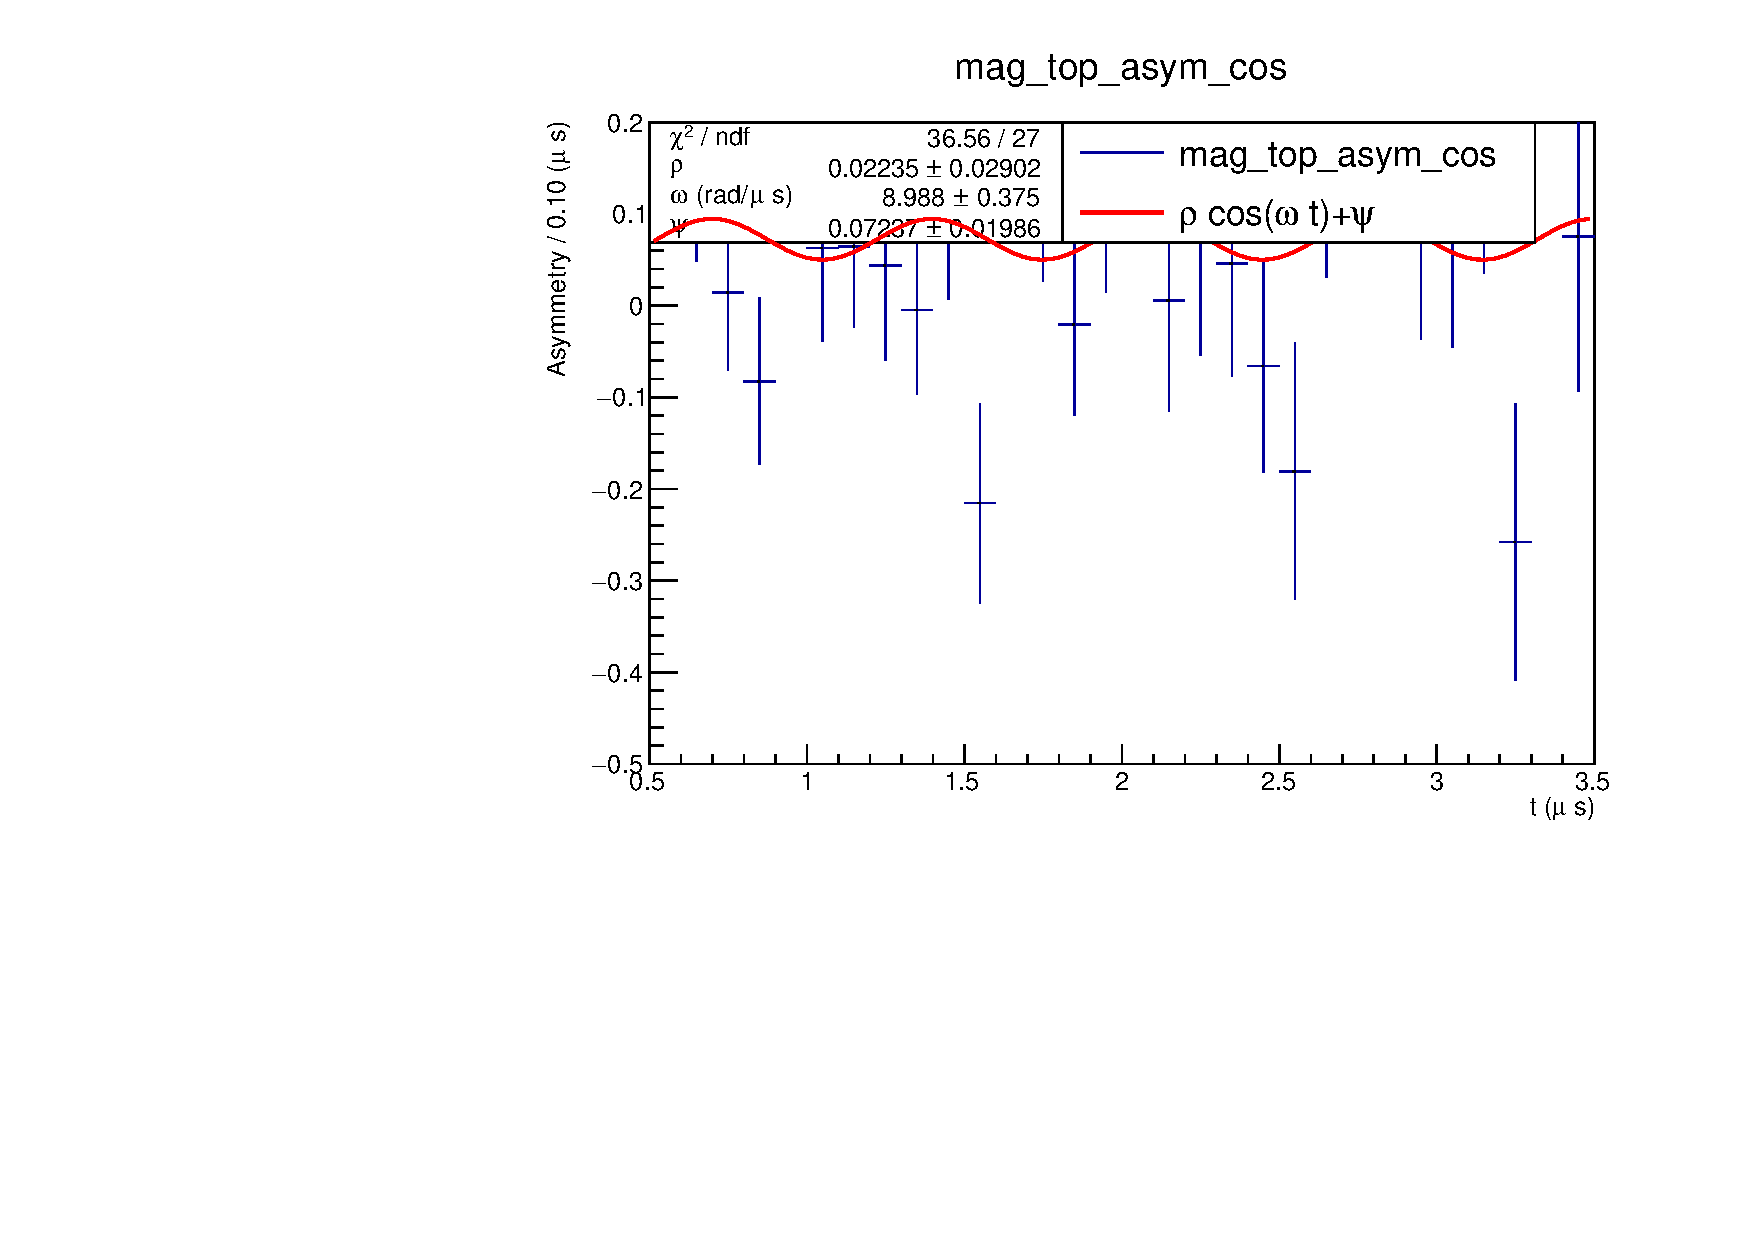
\includegraphics[scale=0.45]{Lab4/Mudecay/mag_top_asym_cos.pdf} 
\label{MAG_TOP_AS}
\end{figure}

\begin{figure}[h!]
\centering
\caption{Asymmetry as a function of time of Mag Fe BOT fitted with a cosine. 18-19-24/05/22]}
\includegraphics[scale=0.45]{Lab4/Mudecay/mag_bottom_asym_cos.pdf} 
\label{MAG_BOT_AS}
\end{figure}

\begin{figure}[h!]
\centering
\caption{Asymmetry as a function of time of Mag Fe TOP fitted with a constant. [25-26-30/05/22]}
\includegraphics[scale=0.45]{Lab4/Mudecay/mag_top_asym_const.pdf} 
\label{MAG_TOP_AS_CONST}
\end{figure}

\begin{figure}[h!]
\centering
\caption{Asymmetry as a function of time of Mag Fe BOT fitted with a constant. 18-19-24/05/22]}
\includegraphics[scale=0.45]{Lab4/Mudecay/mag_bottom_asym_const.pdf} 
\label{MAG_BOT_AS_CONST}
\end{figure}

The various $\chi^2$ are : $\chi^2_{BOT \, cos} = 27.2$,  $\chi^2_{BOT \, const} = 35$, $\chi^2_{TOP \, cos} = 36.6$,  $\chi^2_{TOP \, const} = 37.1$. Here the situation is the same as in the case of $\tau_-$, only now the null Hp is the constant and the alternative is a non null coefficient in front of the sinusoidal (1 DOF). The $\Delta \chi^2$ are 7.8 and 0.5. The second does not reject the constant Hp, while the first one has a p-value$\simeq$0.005, rejecting the constant Hp at $\alpha=0.05$.

Having refuted the constant Hp in the first case, one can also evaluate with the value of the $\chi^2$ itself the goodness of fit of the alternative model. In this case $\chi^2_{BOT, cos}$ is 27.21/27, so a great goodness of fit (p-value $\simeq$ 0.45).
\\
\\
The angular frequency expected from the Larmor precession is 

\begin{equation}
    \omega_L=\frac{eB}{m_\mu}
\end{equation}

\noindent It is difficult to measure the magnetic field inside a magnetic loop, but it can be estimated to be around 100 Gauss, give or take an order of magnitude. With such value the $\omega$ would be 

\begin{equation*}
    \omega_L\sim 9 \text{rad/$\mu$s}
\end{equation*}

Both fitted values for $\omega$ in Mag Fe are compatible within an error bar with $\omega_L$, even while having only 2-3\% relative uncertainty. This is good evidence of the fact that this truly is Larmor precession and that the strength of $B$ is around 100 Gauss.  
    





\subsection{$A(t)$ in NaCl}

In order to test if the oscillation is due to magnetic field and is not a feature of the apparatus, the same procedure is executed with NaCl. This particular material depolarizes the muons with the fields due to interactions between its nuclei. This guarantees that the observed decays are isotropic and, given the absence of a magnetic field, the oscillation should disappear (Figure \ref{NACL_TOP_AS}  \ref{NACL_BOT_AS}) \ref{NACL_TOP_AS_CONST}  \ref{NACL_BOT_AS_CONST}). This means that $A(t)$ should be a constant $\delta$ and if it isn't zero it is purely due to the asymmetries in the \textit{detector} between up and down.
\\
The $\chi^2$ of the fits are: $\chi^2_{BOT \, cos} = 29.1$,  $\chi^2_{BOT \, const} = 32.8$, $\chi^2_{TOP \, cos} = 40.8$,  $\chi^2_{TOP \, const} = 44$.
\\
\\
The $\Delta \chi^2$ are 3.7 and 3.2 with 1 DOF, which corresponds to p-values 0.054 and 0.07. Neither of the two are oscillating enough to refute the constant at 0.05 significance, which confirms our interpretation.
\\
\\
The value of the BOT fitted constant is $\delta_{NaCl,B}=-0.21 \pm 0.01$, which indicates an asymmetry in UP/DOWN detection in the BOT slot. 

Likewise,  $\delta_{NaCl,T}=0.026 \pm 0.017$, which barely suggests a detection asymmetry in the TOP slot.


\begin{figure}[h!]
\centering
\caption{Asymmetry as a function of time of NaCl TOP fitted with a cosine. [18-19-24/05/22]}
\includegraphics[scale=0.45]{Lab4/Mudecay/nacl_top_asym_cos.pdf} 
\label{NACL_TOP_AS}
\end{figure}

\begin{figure}[h!]
\centering
\caption{Asymmetry as a function of time of NaCl BOT fitted with a cosine. [25-26-30/05/22]}
\includegraphics[scale=0.45]{Lab4/Mudecay/nacl_bottom_asym_cos.pdf} 
\label{NACL_BOT_AS}
\end{figure}

\begin{figure}[h!]
\centering
\caption{Asymmetry as a function of time of NaCl TOP fitted with a constant. [18-19-24/05/22]}
\includegraphics[scale=0.45]{Lab4/Mudecay/nacl_top_asym_const.pdf} 
\label{NACL_TOP_AS_CONST}
\end{figure}

\begin{figure}[h!]
\centering
\caption{Asymmetry as a function of time of NaCl BOT fitted with a constant. [25-26-30/05/22]}
\includegraphics[scale=0.45]{Lab4/Mudecay/nacl_bottom_asym_const.pdf} 
\label{NACL_BOT_AS_CONST}
\end{figure}


\\
\\

\subsection{$A(t)$ for Mag Fe-NaCl}

The asymmetry of Nacl is also subtracted from the one of Mag Fe in order to eliminate the effects of the apparatus (Figure \ref{SUB_TOP_AS}  \ref{SUB_BOT_AS} \ref{SUB_TOP_AS_CONST}  \ref{SUB_BOT_AS_CONST}). 
\\
The $\chi^2$ of the fits are: $\chi^2_{BOT \, cos} = 16$,  $\chi^2_{BOT \, const} = 15.6$, $\chi^2_{TOP \, cos} = 35.03$,  $\chi^2_{TOP \, const} = 35.03$. 
\\
\\
These correspond to p values $p_B\simeq 0.53$ and $p_T\simeq 1$, which definitely do not refute a constant
\\
These results are very concerning, because the oscillation disappears from the mag slab if the NaCl is subtracted from it, while it should, in our theory, only shift its baseline.

Evidently we are not at the level of statistics or precision required to be able to distinguish real oscillations from simple constants. This is further suggested by the fact that Mag Fe doesn't appear to oscillate for the TOP slot.

\begin{figure}[h!]
\centering
\caption{Asymmetry as a function of time when subtracting Nacl from Mag Fe TOP fitted with a cosine. [18-19-24-25-26-30/05/22]}
\includegraphics[scale=0.45]{Lab4/Mudecay/top_sub_asym_cos.pdf} 
\label{SUB_TOP_AS}
\end{figure}

\begin{figure}[h!]
\centering
\caption{Asymmetry as a function of time when subtracting Nacl from Mag Fe BOT fitted with a cosine. [18-19-24-25-26-30/05/22]}
\includegraphics[scale=0.45]{Lab4/Mudecay/bottom_sub_asym_cos.pdf} 
\label{SUB_BOT_AS}
\end{figure}

\begin{figure}[h!]
\centering
\caption{Asymmetry as a function of time when subtracting Nacl from Mag Fe TOP fitted with a constant. [18-19-24-25-26-30/05/22]}
\includegraphics[scale=0.45]{Lab4/Mudecay/top_sub_asym_const.pdf} 
\label{SUB_TOP_AS_CONST}
\end{figure}

\begin{figure}[h!]
\centering
\caption{Asymmetry as a function of time when subtracting Nacl from Mag Fe BOT fitted with a constant. [18-19-24-25-26-30/05/22]}
\includegraphics[scale=0.45]{Lab4/Mudecay/bottom_sub_asym_const.pdf} 
\label{SUB_BOT_AS_CONST}
\end{figure}

\\ 
\\

\subsection{$A(t)$ in different materials}



If our theory is correct and muons really are polarized $A(t)$ should be constant but \textit{not} the same constant as NaCl, for that is the \textit{unpolarized baseline}.
\\
\\
For example for Fe the measurements made are shown in Figures \ref{FE_AS_COS},\ref{FE_AS_CONST},\ref{FE_SUB_AS_COS},\ref{FE_SUB_AS_CONST}.



\begin{figure}[h!]
\centering
\caption{Asymmetry as a function of time of Fe TOP fitted with a cosine. [10-11-12-17-19-26/05/22]}
\includegraphics[scale=0.45]{Lab4/Mudecay/fe_top_asym_cos.pdf} 
\label{FE_AS_COS}
\end{figure}

\begin{figure}[h!]
\centering
\caption{Asymmetry as a function of time of Fe TOP fitted with a constant. [10-11-12-17-19-26/05/22]}
\includegraphics[scale=0.45]{Lab4/Mudecay/fe_top_asym_const.pdf} 
\label{FE_AS_CONST}
\end{figure}

\begin{figure}[h!]
\centering
\caption{Asymmetry as a function of time when subtracting Nacl from Fe TOP with a cosine. [10-11-12-17-19-26/05/22]}
\includegraphics[scale=0.45]{Lab4/Mudecay/fe_sub_asym_cos.pdf} 
\label{FE_SUB_AS_COS}
\end{figure}

\begin{figure}[h!]
\centering
\caption{Asymmetry as a function of time when subtracting Nacl from Fe TOP with a cosine. [10-11-12-17-19-26/05/22]}
\includegraphics[scale=0.45]{Lab4/Mudecay/fe_sub_asym_const.pdf} 
\label{FE_SUB_AS_CONST}
\end{figure}


The $\Delta \chi^2$ are barely over 0.05 significance, in line with our theory.

The fitted constant values, that even have a nice goodness of fit value, are  

$$\delta_{Fe,T}=-0.019 \pm 0.011 \quad , \quad \delta_{Fe-NaCl,T}=-0.045 \pm 0.020$$

The TOP value is incompatible with the NaCl one, as can be seen by the fact that the subtracted one is not compatible with zero. This is predicted by our theory. However, our theory predicts that the number of $e^\pm$ should be greater upwards for incoming $\mu^\pm$, so $\delta_{Fe-NaCl,T}$ should be \textit{positive}, not negative




\\
\\
An interesting case is the one of Pb (Figure \ref{PB_AS_COS}) because, even though there appears to be an oscillation, such oscillation \textbf{doesn't show significance}, with respect to a constant fit ($\chi^2 = 41$) shown in Figure \ref{PB_AS_CONST} , when fitted with a cosine of null phase ($\chi^2 = 40$).
\\
The constant is $\delta_{Pb,B}=-0.019 \pm 0.011 $, which is incompatible and higher than the $\delta_{NaCl,B}$, which is what would be expected in our framework.





\begin{figure}[h!]
\centering
\caption{Asymmetry as a function of time of Pb Al BOT fitted with a cosine. [12-17/05/22]}
\includegraphics[scale=0.45]{Lab4/Mudecay/pb_bottom_asym_cos.pdf} 
\label{PB_AS_COS}
\end{figure}

\begin{figure}[h!]
\centering
\caption{Asymmetry as a function of time of Pb Al BOT fitted with a constant. [12-17/05/22]}
\includegraphics[scale=0.45]{Lab4/Mudecay/pb_bottom_asym_const.pdf} 
\label{PB_AS_CONST}
\end{figure}


























\section*{DECLARATION OF AUTHENTICITY}
The authors of this work declare that its contents are original and the fruit of their work alone.

\clearpage
\begin{appendices}


\section{Instrumentation}\label{appendix:nimmodules}

\begin{itemize}
\item 7 rectangular plastic oscillators
\item 7 photomultiplier Tubes (PMT) 
\item DE0-NANO board
\item NIM module: Octal Discriminator unit (8 CHS LRS 623A)
\item NIM module: Coincidence unit (LeCroy 465)
\item NIM module: Dual timer unit (CERN N2255)
\item NIM module: Fan-in (NE 4688)
\item NIM module: NIM-TTL adapter (CAEN 89)
\item NIM module: Quad Gate Delay Generator (PS 794)
\item NIM module: AND OR unit (INFN PISA)
\item NIM module: Multiscaler unit 70 MHz (LACE)
\item NIM module: Multiscaler unit 100 MHz
\item NIM module: Delay units  64-100 ns (CAEN/INFN/CERN PISA)
\item Tektronix dual channel oscilloscope TBS 1102B-EDU
        
 \end{itemize}
 
 
\section{Stopping time for $\mu$}\label{appendix:stoptime}
For an non-relativistic and not radiating ($E_c \sim 1 \text{TeV}$ for muons) particle like $\mu$ the energy loss per unit length of material can be approximated with


\begin{equation}
    \frac{dE}{dx}\simeq-\frac{Kz^2}{\beta^2}
\end{equation}

where $K=1.7$ MeV cm$^{-1}$, $z$ is the charge in $e$, and $\beta$ is the velocity.

In this relativistic limit for a muon

\begin{equation}
    E\simeq\frac{1}{2}m\beta^2+m   \longrightarrow m\beta \frac{d\beta}{dx}=-\frac{K}{\beta^2}  
\end{equation}

Hence

\begin{equation}
    -\frac{m}{K}\beta^2d\beta\simeq \frac{dx}{dx/cdt}=cdt   \longrightarrow t(\beta)\simeq\frac{m}{3cK}(\beta_0^3-\beta^3)
\end{equation}

where $\beta_0$ is the starting velocity when entering the material. The total stopping time is then equal to 
\begin{equation}
     t_{stop}\simeq\frac{m}{3cK}\beta_0^3
\end{equation}

This number, even with $\beta_0=1$ is still only $\simeq 0.7$ ns, which is completely negligible compared to the other time scales in question

In this approximation the energy loss profile for low $\beta$, where the profile is not $\propto 1/\beta^2$, has been neglected. This is because the fraction of time in which the muon has said velocity is expected to 
be negligible compared to the total stopping time.

\section{Combinatorial background}
\label{appendix:combinatorial}

The expected value for combinatorial background is calculated and compared to measured results for data coming from a single Fe run, shown in Figure \ref{Feruncomb}.

\begin{figure}[h!]
\centering
\caption{Time distribution of Fe TOP UP. [26/05/22]}
\includegraphics[scale=0.45]{Lab4/Mudecay/fe_top_up_run11.pdf} 
\label{Feruncomb}
\end{figure}


Using a multiscaler the frequencies of $5\cdot 6$ and $3\cdot 4$ are sampled individually. Over the course of the run in question in particular, $N_{34}= 244067$ counts of $3\cdot 4$ coincidences were measured in the span of $T=10000$ seconds. Assuming a Poissonian distribution, the MLE for its average $\mu_T$ in such time interval is $N_{34}$ itself. The standard deviation of this estimator is $\sqrt{\mu_T}\simeq\sqrt{N}$.

This number of counts is much greater than the number of STOPDOWN = 178 events in the same time frame. Therefore in the following calculations the signal component of $N$ (which should be exponentially distributed) will be neglected.
\\
\\
Selecting a 10 $\mu$s time frame $\Delta t$ in the distribution, e.g. from 10 to 20 $\mu$s, the number of $3\cdot 4$ coincidences expected in the time frame is 

\begin{equation}
    \mu_{\Delta t}=\mu_T\frac{10\mu\text{s}}{T}\simeq 2 \cdot 10^{-4}
\end{equation}

Hence every time there is a START and the GATE sweeps for 30 $\mu$s there is a chance

\begin{equation}
    \mathcal{P}(1;\mu_{\Delta t})=e^{-\mu_{\Delta t}}\mu_{\Delta t}\simeq \mu_{\Delta t}
\end{equation}

of there being one of these casual events in the $\Delta t$ of one START. 
\\
Neglecting $\mathcal{P}(k>1,\mu_{\Delta t})$, the \textit{total} number of such events in the [10,20] $\mu$s time frame of STOPDOWN  $N_{\Delta t}$ is distributed binomially

\begin{equation}
    N_{\Delta t}\sim \mathecal{B}(N_{\Delta t};\mu_{\Delta t},N_S)
\end{equation}

where $N_S$ is the total number of START events in the run, in this case equal to $N_S= 550951$. The $N_{\Delta t}$ expected is then 

\begin{equation}
    N_{\Delta t}= N_S \mu_{\Delta t}\pm \sqrt{N_S \mu_{\Delta t}(1-\mu_{\Delta t)}}=110 \pm 10
\end{equation}

The observed counts in such time frame over the course of $T$ were

\begin{equation}
    N^{obs}_{\Delta t}=115
\end{equation}

which is less than a standard deviation from the expected value of the Binomial.


\section{Fit method}
\label{appendix:fitmethods}
The time distributions were fitted using the functions \ref{expo_long} and \ref{expo_tot} in order to measure respectively $\tau_+$ and $\tau_-$.
In both cases a binned likelihood fit was performed using ROOT's \texttt{Minuit} package. The integral of the function in each bin was used instead of the (default) bin center value. To achieve this the option \texttt{"L I"} in ROOT's \verb#TH1::FiT()# were used.
\\
\\
When dealing with the asymmetry the binned likelihood fit method is no longer valid since the data in the asymmetry histograms does \textit{not} represent counts anymore. For this reason the chi-square fitting method was used, approximating the original $n_{UP/DOWN}$ bin value as distributed Gaussianly from the central limit theorem. Then the bin values for $A(t)$ were taken to be gaussian as well, so a chi-square fit is adequate.


\section{Slab thickness}
\label{appendix:slabthickness}

The thickness of the material slabs used to stop muons plays a dual role in the frequency of STOP events observed for said material. This is because the thicker the slab, the higher the number of muons that have too little energy to cross the slab. But at the same time the thicker the slab the harder it is for eventual decay $e^\pm$ to escape the material. Considering that the range of an electron with an energy of the order of tens of MeV (typical energies of $e^\pm$ coming from $\mu$ decays \cite{e-article}), in iron and aluminum thicknesses of the order of a few centimeters were chosen. Since most $e^\pm$ will not actually go through the entire slab, a thickness of the order of the total range was considered a reasonable choice. The thicknesses tested for Fe and Al were 4 sheets (1.7 cm of Fe, 2.7 cm of Al) and 2 sheets. Comparing the data the STOP signal counts in the case of 4 sheets are around 30\% greater than the 2 sheet case. For this reason in the final runs the number of slabs was always 4 when possible.

For Pb+Al the thickness used is always of 4 sheets (about 1.6 cm).


\twocolumn[
  \begin{@twocolumnfalse}
    \section{Run list}
    \label{appendix:runs}
    \begin{table}[h]
    \centering
    \begin{tabular}{|c|c|c|c|}
    \hline
    Run & Materials & Date & Duration \\
    \hline
    
    Run 1 &  Fe TOP (1.7 cm) & 10/05/2022 & $\sim 115$ hrs\\
    Run 2 &  Fe TOP (1.7 cm) & 11/05/2022 & $\sim 14$ hrs\\
    Run 3 &  Fe TOP (1.7 cm) $\vert$ Pb+Al BOT (1.6 cm) & 12/05/2022 & $\sim 28$ hrs\\
    Run 4 &  Fe TOP (1.7 cm) $\vert$ Pb+Al BOT (1.6 cm) & 17/05/2022 & $\sim 115$ hrs\\
    Run 5 &  NaCl TOP(5 cm) $\vert$ Mag Fe BOT & 18/05/2022 & $\sim 14$ hrs\\
    Run 6 & NaCl TOP(5 cm) $\vert$ Mag Fe BOT & 18/05/2022 & $\sim 1$ hrs\\
    Run 7 &  Fe TOP (0.85 cm) $\vert$ Al BOT (1.35 cm) & 19/05/2022 & $\sim 28$ hrs\\
    Run 8 &  NaCl TOP(5 cm) $\vert$ Mag Fe BOT & 19/05/2022 & $\sim 3$ hrs\\
    Run 9 & NaCl TOP(5 cm) $\vert$ Mag Fe BOT & 24/05/2022 & $\sim 115$ hrs\\
    Run 10 &  Mag Fe TOP $\vert$ NaCl BOT (5 cm) & 25/05/2022 & $\sim 14$ hrs\\
    Run 11 &  Fe TOP (1.7 cm) $\vert$ Al BOT (2.7 cm) & 26/05/2022 & $\sim 28$ hrs\\
    Run 12 &  Mag Fe TOP $\vert$ NaCl BOT (5 cm) & 26/05/2022 & $\sim 3$ hrs\\
    Run 13 &  Afterpulse $\rightarrow$ Mag Fe TOP $\vert$ NaCl BOT (5 cm) & 27/05/2022 & $\sim 14$ hrs\\
    Run 14 &  Mag Fe TOP $\vert$ NaCl BOT (5 cm) & 30/05/2022 & $\sim 70$ hrs\\
    
    \hline
    \end{tabular} 
    \label{signaltable}
    \end{table}


  \end{@twocolumnfalse}




\end{appendices}




\begin{thebibliography}{9}
\bibitem{CMSarticle}
 \textit{Measurement of the charge ratio of atmospheric muons with the CMS detector}, \textbf{CMS}, arXiv:1005.5332v1

\bibitem{e-article}
 \textit{A simple setup to measure muon lifetime and electron energy spectrum of
muon decay and its Monte Carlo simulation} \textbf{arxiv.org/abs/1608.06936v1}

\bibitem{PDG_spectrum}
    \textit{K.Nakamura et al.(Particle Data Group). J. Phys. G 37, 075021 (2010)}

\bibitem{PDGtau}
    \textit{P.A. Zyla et al. (Particle Data Group), Prog. Theor. Exp. Phys. 2020, 083C01 (2020)}
    
    
\bibitem{mupolarized}
    \textit{Polarization of Cosmic-Ray Muons at Sea Level}, C. Scott Johnson, Phys. Rev. \textbf{122}, 1883

\bibitem{afterpulse1}
    \textit{A theory of afterpulse formation in photomultipliers and the prepulse height distribution}, P B Coates 1973 J. Phys. D: Appl. Phys. 6 1862    

\bibitem{afterpulse2}
    \textit{Study of afterpulse effects in photomultipliers}, S. Torre, Review of Scientific Instruments 54, 1777 (1983)
    \textbf{https://doi.org/10.1063/1.1137332}

    
\end{thebibliography}



\end{document} 